\documentclass[bac, screen]{bai-thesis}
\usepackage{thesis}

%-------------------------------------------------------------------------------
% Packages and macros
%-------------------------------------------------------------------------------
\usepackage{verbatim}
\usepackage{subcaption}
\graphicspath{{figures/}}
\setlength{\emergencystretch}{2em}

% Draft markers for the parts that depend on the quantisation grid.
% Set \showtodosfalse before submission: every \todo box disappears and every
% \tbd prints a visible "??" so that nothing unfilled can slip through silently.
\newif\ifshowtodos
\showtodostrue
\ifshowtodos
  \newcommand{\todo}[1]{\par\smallskip\noindent\fcolorbox{orange}{orange!8}{%
    \parbox{\dimexpr\linewidth-2\fboxsep-2\fboxrule\relax}{\small
    \textbf{\textcolor{orange!70!black}{TO DO.}} #1}}\par\smallskip}
  \newcommand{\tbd}{\textcolor{orange!80!black}{\textbf{[--]}}}
\else
  \newcommand{\todo}[1]{}
  \newcommand{\tbd}{??}
\fi

%-------------------------------------------------------------------------------
% Title information
%-------------------------------------------------------------------------------
\title{Quantization and Spike-Based Explainability in Spiking Neural Networks
for Gravitational-Wave Glitch Classification}

\author{Mucaj Deva}
\date{\today}

% Select the subject
\subject{Artificial Intelligence}

% Academic Year
\AY{2025/2026}

\supervisor{Claudio Zandron, Department of Informatics, Systems and Communication, UniMiB}
\supervisor{Davide Gerosa, Department of Physiscs "Giuseppe Occhialini"}
%-------------------------------------------------------------------------------

%-------------------------------------------------------------------------------
\begin{document}
\maketitle
%-------------------------------------------------------------------------------
% \frontmatter
%-------------------------------------------------------------------------------
\chapter*{Abstract}
\addcontentsline{toc}{chapter}{Abstract}

Quantization makes a neural network cheap enough to deploy, and it is usually
validated by checking that accuracy does not fall. On convolutional networks,
accuracy has been shown to survive quantization while the explanations of the
model's decisions do not. This thesis asks the spiking analogue: \emph{does a
quantized spiking neural network base its decisions on the same evidence as its
full-precision counterpart, and at what energy cost?} A spiking network carries
a membrane potential that can be quantized independently of the weights, and its
explanations are sequences of maps; the working hypothesis is that quantizing
the membrane degrades the temporal structure of an explanation before
quantizing the weights degrades its spatial structure.

A four-block convolutional spiking network is trained on four classes of
transient noise from the LIGO Gravity Spy release, reaching $0.9833 \pm 0.0014$
validation accuracy over three seeds under hardware-realizable constraints, and
its decisions are explained with the gradient-free Spike Activation Map. Before
any comparison, the explanation metrics are calibrated: two full-precision
models differing only in seed produce maps correlating at $0.153$ on the worst
class, against a numerical floor of $0.975$. Spatial metrics are therefore valid
only between a model and its own parent, and every quantized model is
fine-tuned from, and compared with, the full-precision model of its own seed.

Weights only, membrane only, and both are quantized at 8, 4 and 2 bits. At 8
and 4 bits accuracy and explanations stay at the level of the parent in every
arm. At 2 bits the arms separate: ternary weights collapse the classifier, while
a 2-bit membrane keeps accuracy at parity ($0.982$) and yet changes the
explanation, whose highlighted region overlaps the parent's by $0.44$ against a
floor of $0.70$ --- a change the spatial correlation ($0.92$) would have reported
as a preserved explanation. The new maps remain faithful by the deletion metric:
they point at evidence the model uses, but not at the evidence the original
pointed at. The hypothesis is not supported as an ordering of explanation
metrics, but its mechanism is: the 2-bit membrane makes the spike trains of the
first layer perfectly periodic, a temporal change the explanation's temporal
metric cannot see. That configuration is also dominated on energy and memory, so
there is no trade-off between efficiency and explainability here: a joint 4-bit
model keeps both at about one sixtieth of the estimated energy and one eighth of
the memory of its parent.

% \cleardoublepage
\phantomsection
\pdfbookmark[0]{Contents}{contents}
\setcounter{tocdepth}{2}
\tableofcontents

% %% Uncomment this for a separate list of figures
% \phantomsection
% \pdfbookmark[1]{List of Figures}{listoffigures}
% \listoffigures

% %% Uncomment this for a separate list of tables
% \phantomsection
% \pdfbookmark[1]{List of Tables}{listoftables}
% \listoftables

% %% Uncomment this for a separate list of algorithms
% \phantomsection
% \pdfbookmark[1]{List of Algorithms}{listofalgorithms}
% \listofalgorithms
%-------------------------------------------------------------------------------
% \mainmatter
%-------------------------------------------------------------------------------
\chapter{Introduction}
\label{ch:introduction}

\section{Motivation}

In 2015 LIGO (Laser Interferometer Gravitational-Wave Observatory) detected
for the first time the collision of two black holes, and in 2017 the gravitational wave
signal GW170817 measured by LIGO and Virgo demonstrated that the fusion of
neutron stars could be observed via telescopes.

Since then, gravitational waves have become a continuous stream of data requiring analysis,
often in real time. In this context, the real challenge is not the faintness of the signals but the noise.
The detectors are so sensitive that they constantly record instrumental and environmental
disturbances known as "glitches".

This is the purpose of Gravity Spy, the source of the data used in this project: to identify
glitch families and trace them back to their causes, as recognizing a glitch
helps in correcting the instrument.

Meanwhile, machine learning has become indispensable for managing data quality,
though it brings with it a cost-related challenge. The demand for computing power
is growing faster than available resources, alerts must be issued within minutes,
and the volume of data is set to increase further.

It is only natural to want to make models more lightweight, and this is where
quantization and spiking neural networks come into play, as they were specifically
designed for low energy consumption.

Deploying a neural network outside a data centre means making it smaller. The
standard tool is indeed quantization, a practice that involves representing weights and activations with fewer
bits, trading numerical precision for memory and energy. The operation is
routinely validated by checking that accuracy does not fall, and for many
applications that is a sufficient test.

Npnetheless, it is not sufficient when the model is used to explain something. Rabbi et
al.~\cite{rabbi2026} evaluated five convolutional architectures at INT8 and
INT4, comparing the attribution maps of the quantized models with those of their
full-precision counterparts. They found that explanation similarity degrades
measurably between INT8 and INT4 even where accuracy differences are negligible,
and that when quantization does cause a misclassification, the quantized model
is generally attending to \emph{different} regions of the input rather than
weighing the same evidence differently. Accuracy and interpretability, in other
words, do not degrade together.

That finding is confined to conventional artificial neural networks. Spiking
neural networks (SNNs), the architecture most closely associated with low-power
deployment~\cite{roy2019towards}, differ from them in ways that make the
question both harder and more interesting.

\section{Research question}

The question this thesis addresses is:

\begin{quote}
\emph{Does a quantized spiking neural network under edge-realistic constraints
base its decisions on the same evidence as its full-precision counterpart, and
at what energy cost?}
\end{quote}

Three properties of spiking networks have no counterpart in the convolutional
setting, and each one bears on the question.

\paragraph{A second quantization target.} A spiking neuron carries a membrane
potential: a state variable read and written at every time step, and a dominant
memory cost at deployment. It is quantized independently of the
weights~\cite{yin2024mint, smith2026}, whereas a conventional network offers only
weights and activations. The two targets can therefore be separated, which turns
a single observation into a causal ablation.

\paragraph{A temporal axis in the explanation.} A spiking explanation is a
\emph{sequence} of maps, one per time step. Quantization may preserve where a
network looks while displacing when it decides, a change to which spatial
metrics are blind by construction.

\paragraph{A native explainer.} The Spike Activation Map~\cite{kim2021sam}
reads spike activity directly. It requires neither gradients, side-stepping the
approximation error a surrogate gradient injects into any transplanted
Grad-CAM-style method~\cite{selvaraju2017gradcam}, nor ground-truth labels.

The working hypothesis follows from the first two properties:

\begin{quote}
\textbf{Quantizing the membrane potential degrades the temporal structure of the
explanation before quantizing the weights degrades its spatial structure},
\end{quote}

since the membrane potential is the variable that integrates evidence over time,
while a weight error is fixed for a whole forward pass. The hypothesis is
falsifiable, and testing it requires quantizing the two targets separately: the
membrane arm should displace the temporal centre of mass of the explanation at a
\emph{higher} bit-width than the one at which the weight arm lowers its spatial
correlation. If the order is reversed, the hypothesis is refuted, which is itself
a reportable result.

\section{Contributions}

Answering the research question requires an instrument, and the metrics used to
compare explanations return numbers between zero and one whatever is fed to them.
Before a quantization result can be read, one must know what those metrics report
when nothing has changed. The thesis is therefore organized in two parts: the
construction and calibration of the instrument, and its application to the
quantization grid.

\begin{enumerate}
  \item \textbf{A hardware-realizable full-precision baseline}, with every
        design choice settled on evidence and recorded in a frozen manifest: the
        input resolution chosen on network health rather than accuracy, the
        membrane decay restricted to shift-implementable values inside the
        hyperparameter search rather than rounded afterwards, and a three-seed
        reference at $0.9833 \pm 0.0014$ validation accuracy.

  \item \textbf{A corrected implementation of the Spike Activation Map}, with
        its decay parameter fixed on the temporal axis it actually governs, and
        its faithfulness tested quantitatively against a random baseline rather
        than judged by visual plausibility.

  \item \textbf{A calibration of the explanation-divergence metrics} at three
        levels: numerical noise, a thirtyfold change in the explainer, and
        initialization variance. Neither of the two closest
        works~\cite{rabbi2026, smith2026} establishes any of the three, and the
        result has the widest scope of the thesis: spatial metrics are valid only
        between a model and its own parent.

  \item \textbf{A bit-width characterization of explanation fidelity for a
        spiking classifier}, with weight and membrane quantization separated and
        then combined, measured with spatial and temporal divergence metrics read
        against the calibrated thresholds, reported per class, and stratified by
        event strength.

  \item \textbf{An analytical energy and memory account} of every operating
        point, so that accuracy, explanation fidelity and energy can be read on
        a common bit-width axis.
\end{enumerate}

\todo{Once the grid is complete, add two or three sentences here stating the
central quantization result (hypothesis confirmed or refuted, and at which
bit-width), mirroring the abstract.}

\section{Application domain}

The classification task is the identification of transient noise --- known as
\emph{glitches} --- in the data of the LIGO gravitational-wave detectors, using
the Gravity Spy release~\cite{zevin2017, glanzer2023, glanzer2021}.

The domain was chosen for three reasons. Explanation fidelity has an
\emph{operational} consequence there: glitch classification guides detector
characterization, where a commissioner acts physically on the instrument, so a
compressed model reaching the same label from different evidence would preserve
the label while corrupting the diagnostic cue. The classes have physically
interpretable morphology, so a domain expert can judge whether an attention map
falls where the glitch actually is, which is not true of a generic image
benchmark. And the data is public, large and labelled.

\section{Scope}

This work characterizes explanation fidelity under \emph{simulated}
quantization, with analytical energy and memory accounting. Hardware deployment
is explicitly out of scope: no model is exported to a neuromorphic device or
microcontroller, and no latency or power is measured on one.

Every design decision in this thesis is taken on the validation partition. The
test partition is opened once, for the final estimates reported in
Section~\ref{sec:test}.

\section{Structure}

Chapter~\ref{ch:background} reviews spiking neural networks, their training by
surrogate gradients, quantization for spiking architectures, explainability
methods applicable to them, and the gravitational-wave classification task.
Chapter~\ref{ch:methodology} describes the data pipeline, the model, the
selection of the operating configuration, the Spike Activation Map and the
protocol used to calibrate the divergence metrics.
Chapter~\ref{ch:quantization} describes the quantization study: the quantizers,
the grid, the fine-tuning protocol, the divergence metrics and the energy model.
Chapter~\ref{ch:results} reports the full-precision reference, the physical
validation of the network dynamics, the explainability analyses, the
calibration, and the results of the quantization grid.
Chapter~\ref{ch:conclusions} discusses the findings and their limits, and
outlines future work.

\chapter{Background and Related Work}
\label{ch:background}

\section{Spiking neural networks}

Spiking neural networks (SNNs) are often described as the third generation of
neural networks~\cite{maass1997networks}. They take their inspiration from biological neurons, which communicate through
brief, all-or-nothing electrical impulses called \emph{spikes}.
In a conventional
ANN, each neuron outputs a continuous value computed once per input, while in an SNN,
information is carried by sequences of binary events distributed over time: at
each of $T$ discrete time steps, a neuron either emits a spike or stays silent.
The network therefore processes an input as a short temporal sequence. This holds
even when the input is static, as with a spectrogram, our specific case, which is presented
repeatedly or encoded as spikes over the $T$ steps.

This representation is exactly what makes SNNs attractive for low-power computing. Because
activations are binary, the multiply--accumulate operations that dominate the cost
of an ANN reduce to simple accumulations, performed only when a spike actually
is fired. Computation is therefore sparse and event-driven, with a silent neuron costing
almost nothing. Neuromorphic processors such as Intel's
Loihi~\cite{davies2018loihi} are built to exploit this sparsity directly, and the
energy advantage of an SNN is set to grow as its firing activity decreases.

The most widely used neuron model in deep SNNs is the leaky integrate-and-fire
(LIF) neuron~\cite{gerstner2014neuronal}. In this configuration, neuron maintains an internal state,
its membrane potential $U$, which
integrates incoming input, decays (``leaks'') towards rest over time, and triggers
a spike when it crosses a threshold $\theta$.

As shown in Figure~\ref{fig:neuron_models}, the LIF model sits between
biologically detailed neuron models and the artificial neurons of
conventional deep learning (ANNs).

\begin{figure}[htbp]
  \centering
  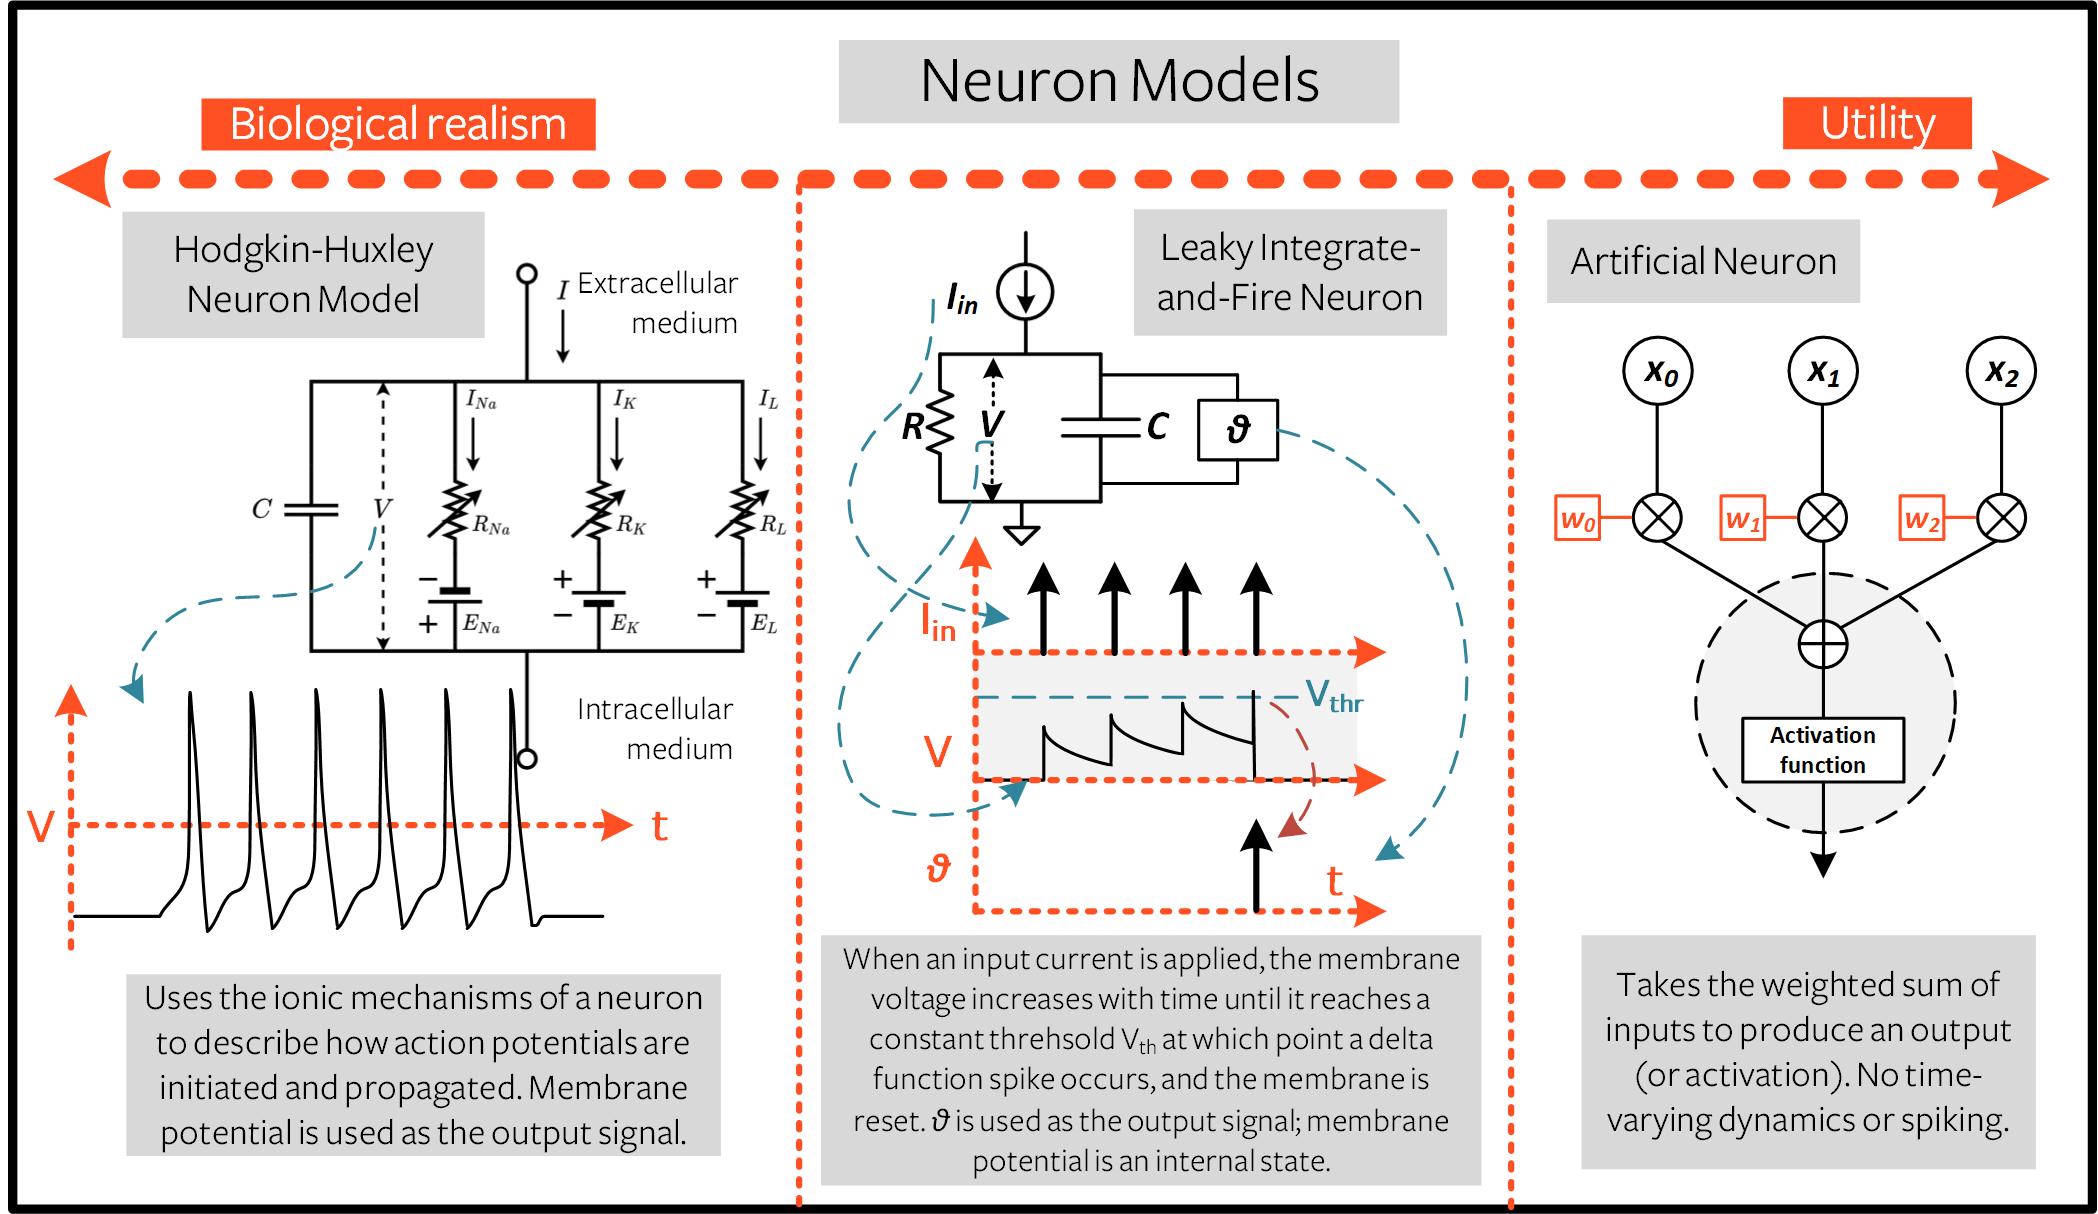
\includegraphics[width=\linewidth]{lif_neuron_models.png}
  \caption[Neuron models: from Hodgkin--Huxley to the artificial neuron]{%
    Neuron models ordered from biological realism to computational
    utility. Left: the Hodgkin--Huxley model describes the generation of
    action potentials through voltage-dependent ionic conductances, at a
    high computational cost. Centre: the leaky integrate-and-fire (LIF)
    neuron reduces the membrane to an RC circuit: the capacitor $C$
    integrates the input current $I_{\mathrm{in}}$, while the resistor $R$ makes
    the stored charge leak away over time, and a spike is emitted when the
    membrane potential reaches the threshold (denoted $\vartheta$ in the
    figure and $\theta$ in the text), after which the potential is reset.
    Unlike the Hodgkin--Huxley model, the membrane potential of a LIF neuron is an internal
    state and the spike is the output. Right: the artificial neuron of
    conventional ANNs, which computes a weighted sum of its inputs followed by an
    activation function, with no temporal dynamics and no spikes.
    Reproduced from the snnTorch documentation~\cite{snntorch_tutorial2}
    (MIT License).}
  \label{fig:neuron_models}
\end{figure}

In the discrete-time formulation used by snnTorch~\cite{eshraghian2023}, the
dynamics of a neuron at time step $t$ are the following
\begin{equation}
  U[t] = \beta\, U[t-1] + W X[t] - S[t-1]\,\theta ,
  \label{eq:lif}
\end{equation}
\begin{equation}
  S[t] =
  \begin{cases}
    1 & \text{if } U[t] > \theta, \\
    0 & \text{otherwise},
  \end{cases}
  \label{eq:spike}
\end{equation}
where $W X[t]$ is the weighted input from the previous layer, $S[t]$ is the binary
output spike, and the subtraction term resets the potential by $\theta$ after each
spike. The decay factor $\beta \in [0,1)$ sets how much of its past state the
neuron retains: values close to $1$ give a long memory, so the neuron integrates
evidence over many time steps; smaller values make it respond mainly to recent
input.

The property of the membrane potential to give the LIF neuron a memory is what separates
it from a stateless activation function: the output at time $t$ depends on the
entire history of inputs up to $t$.
The same mechanism, nonetheless, also creates the main
difficulty in training. The spike function in Eq.~\eqref{eq:spike} is a step
function, whose derivative is zero almost everywhere and undefined at the
threshold, so standard backpropagation cannot pass through it. The usual solution
is the \emph{surrogate gradient} approach~\cite{neftci2019surrogate}: the step
function is kept in the forward pass, but in the backward pass its
derivative is replaced with that of a smooth approximation, such as an arctangent.
Combined with backpropagation through time over the $T$ steps, this allows deep SNNs to
be trained with the same gradient-based tools as conventional networks.

These properties change the quantization problem in three main direct ways. First, SNN
activations are already binary, so the precision that quantization removes lies
in the weights and in the membrane potential, a state variable with no direct
equivalent in an ANN. Second, the threshold makes the network highly sensitive to
small numerical changes. Indeed, a perturbation that moves $U$ slightly above or below
$\theta$ turns a spike into silence, or the reverse. Because the membrane carries
its state forward, such an error does not stay local, but can propagate through
later time steps and layers. Third, explanations of an SNN can be temporal as well
as spatial. The Spike Activation Map (SAM)~\cite{kim2021sam} builds
attribution maps directly from the timing of spikes, without computing
gradients, and therefore show not only \emph{where} the network finds evidence in
the input but also \emph{when} during the $T$ time steps it does so. Whether
quantization preserves this temporal reasoning, and not only accuracy, is the
question this thesis sets out to answer.

\subsection{Training by surrogate gradients}
\label{sec:surrogate}

Unrolled over its $T$ time steps, a network of LIF neurons is effectively a recurrent
network: the membrane potential is a hidden state that each step reads and
updates (Equation~\ref{eq:lif}). Training it by gradient descent requires solving
two credit-assignment problems at once~\cite{neftci2019surrogate}: a
\emph{spatial} one, across layers, as in any multi-layer network, and a
\emph{temporal} one, since a weight influences the loss through every later
state of the neurons it feeds. Backpropagation through time (BPTT) solves both
by applying the chain rule to the unrolled graph. For a weight $W$ feeding a
neuron with potential $U[t]$ and output $S[t]$,
\begin{equation}
\frac{\partial \mathcal{L}}{\partial W}
= \sum_{t} \frac{\partial \mathcal{L}}{\partial S[t]}\,
  \frac{\partial S[t]}{\partial U[t]}\,
  \frac{\partial U[t]}{\partial W},
\qquad
\frac{\partial S[t]}{\partial U[t]} = \Theta'\!\left(U[t] - \theta\right),
\label{eq:bptt}
\end{equation}
where $\Theta$ is the Heaviside step of Equation~\ref{eq:spike} and
$\partial U[t]/\partial W$ is the total derivative through all earlier states.
The price is
memory: every state of every time step must be kept until the backward pass,
a cost that grows as $O(NT)$ for a layer of $N$ neurons.

\paragraph{The obstacle.} Every path through Equation~\ref{eq:bptt} contains the
factor $\Theta'$, which is zero everywhere except at the threshold, where it is
undefined. The gradient is therefore either zero or meaningless: a small change
of a weight almost never flips a spike, so the loss is piecewise constant in the
weights, with flat plateaus on which gradient descent cannot move. This is the
same problem met by networks with binary activations, and the solutions
developed for spiking networks are inspired by those~\cite{neftci2019surrogate}.

\paragraph{The surrogate.} A surrogate gradient leaves the model unchanged and
alters only its derivative. The forward pass keeps the exact binary spike, while in
the backward pass every occurrence of $\Theta'$ is replaced by the derivative
$\sigma'$ of a smooth function peaked at the threshold,
\begin{equation}
\frac{\partial S[t]}{\partial U[t]} \;\longrightarrow\;
\sigma'\!\left(U[t] - \theta\right).
\end{equation}
Neurons close to threshold, meaning those for which a small change could flip a spike,
receive the largest gradient, and gradient flows through silent neurons as well.
The resulting update is the gradient of a
\emph{virtual} surrogate loss, never computed explicitly, which follows the true
one while remaining continuous and finite~\cite{neftci2019surrogate}. This
distinguishes the approach from \emph{smoothed} spiking networks, which involve replacing
the spike itself with a soft or probabilistic function and so change the model
that is deployed.

\paragraph{The choice of surrogate.} Piecewise-linear, fast-sigmoid and
exponential surrogates have all been used successfully, all three sharing non-linearity 
and monotonically increasing towards the threshold. The
diversity of working choices suggests that the method does not depend
critically on the exact shape~\cite{neftci2019surrogate}. This work uses the
arctangent surrogate~\cite{fang2021plif} as implemented in
snnTorch~\cite{eshraghian2023},
\begin{equation}
\sigma'(x) = \frac{\alpha/2}{1 + \left(\frac{\pi}{2}\,\alpha\, x\right)^{2}},
\qquad \alpha = 2,
\end{equation}
which equals $1$ at the threshold and falls off as the inverse square of the
distance from it, so that neurons far from threshold still receive a small,
non-zero gradient. The reset term $-S[t-1]\,\theta$ of
Equation~\ref{eq:lif} is treated as a constant in the backward pass: the
recurrence then contributes $\partial U[t]/\partial U[t-1] = \beta$ alone, without
a second surrogate factor through the reset, a simplification that has been
found empirically to improve training~\cite{neftci2019surrogate}. With this training
configuration, spiking networks can manage to reach accuracies comparable to conventional architectures
on image benchmarks~\cite{eshraghian2023}.

The same device reappears in Section~\ref{sec:quantization-background}: the
straight-through estimator used to train through a rounding
operation~\cite{bengio2013ste} replaces the zero derivative of a step function
with that of a smooth one, exactly as the surrogate gradient does for the spike.

\paragraph{A consequence for explainability.} The substitution motivates the
choice of explanation method in Section~\ref{sec:sam-background}: any
gradient-based attribution computed on such a network inherits the
approximation error of the surrogate, because the gradients it uses are not the
gradients of the function the network actually computes.

\subsection{Input encoding}
\label{sec:encoding}

A spiking network processes its input over $T$ discrete time steps, while an
image is a single static frame, so the frame must be turned into a sequence. In this context, two
strategies dominate. In \emph{rate coding} each normalized pixel intensity is
used as the probability of emitting a spike at every step, and the value is
carried by the spike count; in \emph{direct} (or \emph{constant}) encoding, the
analog frame itself is presented, identical, at every time step.

Rate coding trades its simplicity in time steps: a pixel is represented by
counting spikes, so with $T$ steps it can take only $T + 1$ distinct values, and
the sampling makes the representation stochastic: the discretization error
shrinks only as $T$ grows, which is why rate-coded and converted networks
typically require between $100$ and $2\,000$ time steps to approach the
accuracy of their non-spiking counterparts~\cite{rathi2023dietsnn}.

Direct encoding, as introduced by DIET-SNN~\cite{rathi2023dietsnn}, removes
that error at the source. ``The pixel intensities of an image are applied
directly to the input layer of the SNN at each timestep'', and the first
convolutional layer, followed by LIF neurons, becomes at once a feature
extractor and a learned spike generator: it integrates the weighted pixel
values and fires when its membrane potential crosses threshold. Since the
input carries its full precision at every step, the number of steps is no longer
bounding the precision of the input. DIET-SNN combines this encoding with a
trained membrane leak and firing threshold per layer, which increase activation
sparsity, and reaches $69\,\%$ top-1 accuracy on ImageNet with $5$ time steps
and about $12\times$ less compute energy than the equivalent conventional
network~\cite{rathi2023dietsnn}. This work adopts the encoding but not the
trained neuron parameters: $\beta$ and the threshold are shared by all layers,
and $\beta$ is chosen by the constrained search of
Section~\ref{sec:constrained-search}.

Direct encoding has three remarkable consequences that the rest of this thesis relies on.

\paragraph{Temporal structure is generated inside the network.} Since the
stimulus does not vary, \textbf{all temporal structure in the network
originates from the internal LIF dynamics} --- leak, integration and reset ---
and not from variation in the input. The time axis of a spike train, and
therefore of a Spike Activation Map, is the time the network takes to integrate
evidence, which is not the time of the glitch: in an Omega-scan spectrogram, physical
time runs along the horizontal axis of the image and is, for the network, a
spatial dimension. Every temporal analysis in this thesis is to be read in that
light.

\paragraph{The first layer is the only one that multiplies.} Every other layer
receives binary spikes and only accumulates, but the first convolution receives
analog pixel values and performs full multiply-accumulates. Because its input is
identical at every step, so is its output current, which can be computed once
rather than $T$ times. Section~\ref{sec:energy-method} shows how this choice
 decides whether the spiking network is cheaper than its conventional
equivalent.

\paragraph{The input is deterministic.} Without sampling, two forward passes on
the same image produce identical spike trains, which is what allows two models to
be compared spike for spike on the same input, as the calibration of
Section~\ref{sec:calibration} requires.

\section{Quantization}
\label{sec:quantization-background}

Quantization represents the parameters and intermediate values of a network with
fewer bits than the 32 of floating point. Storing a value in $b$ bits divides its
memory by $32/b$, and integer operations on narrow operands cost far less energy
than floating-point ones (Section~\ref{sec:energy-background}), which is why
quantization is the standard practice adopted between a trained model and its deployment on
constrained hardware~\cite{jacob2018quantization, nagel2021whitepaper}.

\paragraph{The uniform quantizer.} A uniform quantizer maps a real value $x$ to
one of at most $2^b$ equally spaced levels: it divides by a step $\Delta$, rounds to the
nearest integer, clips to the representable range, and multiplies back,
\begin{equation}
\hat{x} = \Delta \cdot \mathrm{clip}\!\left(\mathrm{round}\!\left(\frac{x}{\Delta}\right),
\, q_{\min},\, q_{\max}\right)
\label{eq:quantizer}
\end{equation}

where $q_{\min}$ and $q_{\max}$ are the smallest and largest integer levels
representable with $b$ bits: $-(2^{b-1}-1)$ and $2^{b-1}-1$ for a symmetric
signed grid-- which keeps zero exactly representable at the cost of one unused
code-- $2^b - 1$ levels in all; $0$ and $2^b - 1$ for an unsigned one, which uses
all $2^b$. The largest representable value is therefore $\Delta\, q_{\max}$.

For a symmetric grid over $[-w_{\max}, +w_{\max}]$ the largest level must reach
$w_{\max}$, so the step is
\begin{equation}
\Delta = \frac{w_{\max}}{2^{b-1} - 1} = \frac{2 w_{\max}}{2^b - 2},
\label{eq:step}
\end{equation}
the step the weight quantizer of Chapter~\ref{ch:quantization} computes for each
output channel. Section~\ref{sec:perturbation} expresses a perturbation in a unit
derived from it: the 8-bit step of a single per-tensor grid set by the largest
weight of the whole network, computed there as $2 w_{\max}/(2^8 - 1)$, which is
$0.4\,\%$ smaller than Equation~\ref{eq:step} at 8 bits.
Since the quantizer
works per channel, and most channels have a smaller maximum than the network as
a whole, that unit is coarser than the steps the quantizer actually applies, and
the floor it defines is conservative.

There are two main errors that follow from Equation~\ref{eq:quantizer}, with the choice of range
trades one against the other: values inside the range are moved by at most
$\Delta/2$ (\emph{rounding} error), values outside it are cut to the nearest
bound (\emph{clipping} error). For values spread over many steps the rounding
error is close to uniform on $[-\Delta/2, \Delta/2]$, with a root-mean-square of
$\Delta/\sqrt{12}$; a Gaussian perturbation whose standard deviation is one step,
the unit of Section~\ref{sec:perturbation}, is therefore about $3.5$ times
larger than the rounding it stands for. A wide range avoids clipping but makes
$\Delta$ coarse; a narrow one refines $\Delta$ at the cost of saturating the
tails.

When the quantity is non-negative, or its negative values carry no information
for the task, an \emph{unsigned} grid over $[0, x_{\max}]$, with step
$x_{\max}/(2^b - 1)$, spends no levels on values the network does not use. The
membrane potential of this network is of the second kind. Negative potentials
are frequent --- in the first layer the median is $-0.08$ and the first
percentile $-6.6$ --- yet clipping them to zero moves the validation accuracy by
one image in $1\,435$ (Section~\ref{sec:membrane-prep}).

More specifically, the step can be shared by a whole tensor (\emph{per-tensor}) or computed
separately for each output channel (\emph{per-channel}). A per-tensor step is
set by the largest value in the tensor, so channels whose weights are
systematically smaller use only a fraction of the available levels; the
per-channel scheme avoids this at the price of one scale factor per
channel~\cite{krishnamoorthi2018whitepaper, nagel2021whitepaper}.

Given a quantizer, two families of method decide \emph{when} it is applied:
after training, or during it.

\paragraph{Post-training quantization (PTQ).} PTQ converts an already trained
full-precision model: the weights are rounded to their grid,
and the ranges of the activations, which depend on the data, are estimated on a
small unlabelled calibration set~\cite{nagel2021whitepaper}. It is a relatively fast method and
needs neither labelled data nor a training pipeline, which makes it the
``push-button'' option and the one most used for rapid deployment. Its limit is
precision: at 8 bits the rounding error is small compared with the spread of the
weights, and per-channel PTQ keeps classification accuracy within about 2\,\% of
floating point on standard convolutional networks. At 4 bits the step is sixteen
times coarser, and accuracy typically degrades unless more elaborate correction
methods are used~\cite{krishnamoorthi2018whitepaper, nagel2021whitepaper}. Rabbi et
al.~\cite{rabbi2026} use static weight-only PTQ at INT8 and INT4, the setting in which
they observe explanations degrading before accuracy.

\paragraph{Quantization-aware training (QAT).} QAT includes the quantizer in
training, so that the network can adapt its weights to the grid. Specifically, in the forward pass every quantized tensor is
passed through Equation~\ref{eq:quantizer} --- \emph{simulated} or
\emph{fake} quantization, since the values are rounded but still stored and
processed in floating point --- so that the loss is computed on the network as
it will be deployed~\cite{jacob2018quantization}. The difficulty lies in the backward
pass: rounding is a step function, whose derivative is zero almost everywhere,
and no gradient would reach the weights. The \emph{straight-through estimator}
solves it by treating rounding as the identity in the backward
pass~\cite{bengio2013ste}: the forward pass sees the quantized value, the
gradient flows as if it had not been quantized. This is the same device, in a
different guise, as the surrogate gradient of Section~\ref{sec:surrogate}, which
also keeps a step function in the forward pass and replaces its derivative in
the backward one. QAT needs labelled data and additional training, usually as a
fine-tuning of the full-precision model, and in exchange reaches lower
bit-widths: it narrows the 8-bit gap to about 1\,\% and makes 4-bit weights
usable, with losses between 2 and 10\,\% depending on the size of the
network~\cite{krishnamoorthi2018whitepaper, nagel2021whitepaper}.

The two families therefore answer different needs: PTQ when the model must be
compressed cheaply and 8 bits suffice, QAT when the target precision is lower
than PTQ can reach. In a spiking network both apply not only to the weights but
also to the membrane potential, as the next section describes.

\subsection{Quantization for spiking networks}

Spiking architectures add constraints of their own, as could already be inferred.
The membrane decay $\beta$
multiplies a stored state at every time step, so on integer hardware it is
cheapest when realizable as a bit shift: $\beta = 2^{-k}$ is a right shift, and
$\beta = 1 - 2^{-k}$ is a shift plus a subtraction. MINT~\cite{yin2024mint}
quantizes both targets uniformly and shares a single
scale factor between weights and membrane potentials. Since the weighted input
and the stored state are then expressed in the same integer units, they can be
added directly, and the multipliers that conventional uniform quantization needs
to rescale one into the other disappear from the inference loop. At 2 bits,
MINT reports $90.6\,\%$ accuracy on CIFAR-10 with a VGG-16 and a memory
reduction of $93.8\,\%$ with respect to full precision.
HardF-SNN~\cite{liu2026hardfsnn} shows the cost of that sharing: weights have a
narrow, centred distribution, whereas membrane potentials have a much broader
one with a long tail, so a scale fitted to the weights compresses the dynamic
range of the membrane and collapses many distinct potentials onto the same
level. It therefore scales the membrane in proportion to the weights rather
than identically, replaces batch normalization with an integer, shift-based
version, and verifies the result on an FPGA accelerator, noting that most
quantized spiking networks are still evaluated with simulated quantization, in
which part of the computation remains in floating point.

Smith et al.~\cite{smith2026} argue independently that accuracy is an
insufficient criterion for quantized spiking networks. They in fact propose an Earth
Mover's Distance between per-neuron firing-rate distributions as a diagnostic of
behavioural divergence. Separating weight from membrane quantization as this
thesis does, and reporting that membrane-potential quantization requires at least
four bits to preserve both accuracy and dynamics while learned weight
quantization remains viable at two. They ground the asymmetry mechanistically: a
weight quantization error is fixed for an entire forward pass, whereas a membrane
error propagates through the recurrent update at every time step.

This thesis reaches the opposite result at 2 bits: the membrane arm keeps
accuracy at parity (Section~\ref{sec:grid-results}). A plausible reason is where
the quantizer acts. Here it rounds the state carried into the next step, after
the spike decision (Section~\ref{sec:membrane-quantizer}). At every step the
threshold is compared with $\beta$ times the quantized previous state plus a
full-precision input current, so the comparison itself is never made on a 2-bit
value.

\subsection{Energy and memory accounting}
\label{sec:energy-background}

Since no model is deployed on hardware in this work, energy is estimated
analytically, as is standard in the spiking literature: the operations an
inference requires are counted and multiplied by a per-operation cost at a
reference process node, conventionally the 45\,nm figures of
Horowitz~\cite{horowitz2014}. The result is a
like-for-like comparison between configurations of the same network.

\paragraph{Counting operations.} In a conventional layer every connection
performs one multiply-accumulate (MAC) per inference. In a spiking layer the
input is binary, so a connection only \emph{adds} its weight, and only when the
presynaptic neuron fires. The number of these synaptic operations (SOP) is
therefore the dense MAC count scaled by the firing rate $f$ of the input layer
and by the number of time steps,
\begin{equation}
\mathrm{SOP} = f \cdot T \cdot \mathrm{MAC}.
\end{equation}
In 32-bit floating point a MAC costs $4.6$\,pJ (a $3.7$\,pJ multiplication plus a
$0.9$\,pJ addition) and an accumulate $0.9$\,pJ. That factor of five is the
physical reason a spiking network can be cheaper and lighter, and it also sets the limit:
a spiking layer saves energy only while $f \cdot T < 4.6 / 0.9 \approx 5$, so
sparsity and a short time window are both necessary. The first layer is an
exception, since under direct encoding it receives analog values and performs
full MACs (Section~\ref{sec:encoding}).

\paragraph{Quantized operations.} The same table supplies the integer figures
used for quantized operating points: an 8-bit multiplication costs $0.2$\,pJ and
an 8-bit addition $0.03$\,pJ, thirty times less than its floating-point
counterpart, so that an 8-bit MAC costs $0.23$\,pJ under the same convention
that gives $4.6$\,pJ in floating point. Narrower integer operations are not tabulated, so any figure below
eight bits is an extrapolation, whose rule is stated in
Chapter~\ref{ch:quantization}.

\paragraph{What the count leaves out.} The estimate covers arithmetic only. It
ignores the update of each neuron (leak, threshold comparison, reset), control
logic, and above all data movement, which on real hardware is often the larger
cost: in the same 45\,nm table, reading 64 bits from on-chip SRAM costs between
$10$ and $100$\,pJ depending on its size, and from off-chip DRAM between $1.3$
and $2.6$\,nJ~\cite{horowitz2014}, one to three orders of magnitude more than an
arithmetic operation.

\paragraph{Why memory is accounted separately.} For this reason the memory
footprint is reported alongside the energy estimate:
the energy of an access depends on where the data lives, which is a property of
the hardware, whereas the number of bits to be stored is a property of the
model. The footprint is computed as the bits needed for the weights plus the
bits needed for the membrane state of every neuron. The second term is specific
to spiking networks: a conventional network can discard the activations of a
layer once the next one has been computed, but a spiking network must keep the
potential of every neuron from one time step to the next for the whole
inference. That state scales with the number of neurons rather than the number
of parameters, and it can be quantized independently of the weights
(Section~\ref{sec:quantization-background}).

\section{Explainability for spiking networks}
\label{sec:sam-background}

Attribution methods developed for conventional networks transfer badly to
spiking ones, for two different causes. Gradient-based methods such as
Grad-CAM~\cite{selvaraju2017gradcam} weight feature maps by the gradient of the
class score, and in a spiking network that gradient exists only as a surrogate
(Section~\ref{sec:surrogate}). The approximation is applied again at every layer
the gradient crosses, so the error accumulates with depth: Kim and
Panda~\cite{kim2021sam} observe that Grad-CAM transplanted to spiking networks
produces smoothed, poorly discriminative maps, worst at the shallow layers.
Perturbation methods such as LIME~\cite{ribeiro2016lime} avoid gradients
altogether and are architecture-agnostic, but they need hundreds to thousands of
forward passes per explanation. Both families, moreover, return a single map per input,
and so discard the temporal axis along which a spiking network computes.

\paragraph{The Spike Activation Map.} The Spike Activation Map (SAM) of Kim and
Panda~\cite{kim2021sam} was designed for spiking networks from the start. It
rests on a biological observation: spikes that follow each other at short
inter-spike intervals are more likely to drive the membrane of the downstream
neuron above threshold, and therefore carry more information than isolated
ones. SAM numerically quantifies this into a score computed in three steps. A \emph{temporal
spike contribution score} weights a past spike at $t'$ by its recency with
respect to the current step $t$,
\begin{equation}
T(t, t') = \exp\left(-\gamma\,|t - t'|\right),
\end{equation}
where $\gamma$ sets how fast the contribution of a spike fades. A
\emph{neuronal contribution score} sums these weights over the spikes the neuron
emitted before $t$,
\begin{equation}
N^{k}_{ij,t} = \sum_{t' \in P^{k}_{ij},\; t' < t} T(t, t'),
\end{equation}
where $P^{k}_{ij}$ is the set of firing times of the neuron in channel $k$ at
position $(i,j)$; it is high for a neuron that has fired often and recently, and
low for one that fired rarely or long ago. Finally, the map at time $t$ keeps
the score only of the neurons that are firing at $t$ and sums over the channels
of the layer,
\begin{equation}
M_{ij,t} = \sum_{k} N^{k}_{ij,t}\, S^{k}_{ij,t},
\end{equation}
yielding one spatial heat map per time step and per layer.

\paragraph{Properties.} Several properties of SAM matter for this thesis. It uses
solely the spike trains of the forward pass, so the explanation describes the function the
network actually computes, and its cost is marginal --- a store of recent spike
times and a lookup table for the kernel, which Kim and Panda note could be
implemented in an inference accelerator. It needs no class label: SAM shows
where the network concentrates its activity for a given input, not the evidence
for a particular class, so its faithfulness must be tested against the class
the model predicts. And it has a temporal axis: an explanation is a sequence of
$T$ maps, which is what makes it possible to ask whether quantization changes
\emph{when} a network decides as well as \emph{where} it looks. Kim and Panda
validate the method on Tiny-ImageNet, finding SAM more discriminative than
Grad-CAM adapted to spiking networks.

Feature-attribution methods for spiking networks have also been surveyed more
broadly~\cite{nguyen2023attribution}, but SAM remained the method that reads the
spike trains directly, and it is the explainer used throughout this work. Its
one free parameter, $\gamma$, is fixed in Section~\ref{sec:gamma}.

\subsection{Evaluating an explanation}

A stable explanation can still be wrong, so stability requires a separate test
of faithfulness. The \emph{deletion metric} of Petsiuk et
al.~\cite{petsiuk2018rise} removes pixels in decreasing order of attributed
importance, and records how quickly the model's confidence falls, summarized as
the area under that curve. The faster the fall, the smaller the area. The
underlying hypothesis is that a faithful map degrades the prediction faster than
a map that carries no information. Petsiuk et al. read the area on its own; this
thesis compares it with the removal of pixels in random order on the same image
(Section~\ref{sec:faithfulness}), so that a map counts as faithful only by the
margin it gains over chance.

The metrics used to quantitatively compare two explanations with each other are borrowed from
the saliency-model literature, where they were specifically developed to compare a predicted
map against human eye fixations~\cite{bylinskii2019metrics}: Pearson
correlation, structural similarity~\cite{wang2004ssim}, and the
intersection-over-union of the highest-scoring regions. Bylinskii et al. observe
that rankings produced by different metrics frequently disagree, which is the
main reason for reporting more than one. This thesis reports the correlation and
the overlap. Structural similarity, which Rabbi et al.~\cite{rabbi2026} use
alongside them, is left out as redundant with the two.

A separate line of work asks whether attribution methods are testing anything at
all. Adebayo et al.~\cite{adebayo2018sanity} randomize model weights
progressively and verify that explanations change in response, as a map that
survives the destruction of the model it sets to explain is not explaining
it. The perturbation experiment of Section~\ref{sec:perturbation} is a graded
form of that test, run in the opposite direction.

\section{Gravitational-wave glitch classification}
\label{sec:gravityspy}

The sensitivity of the LIGO interferometers is primarily limited by non-Gaussian transient
noise of instrumental and environmental origin. As introduced in
Chapter~\ref{ch:introduction}, these glitches are short, can mimic astrophysical
signals, and cna be grouped into morphological families that correlate with
distinct physical causes.

The Gravity Spy project~\cite{zevin2017, bahaadini2018} combines machine
classification with citizen science to label them. The release used
here~\cite{glanzer2021} covers observing runs O1 through O3b and provides, for
each Omicron trigger, the trigger metadata, the per-class scores of a
convolutional classifier, the label that classifier assigns, and the addresses
of the Omega-scan spectrograms, which are downloaded separately from the
Zooniverse archive. The labels used in this work are therefore machine labels,
not volunteer consensus, and no threshold on the classifier's confidence was
applied when the data were selected.

The scores released with the labels do not always support them. Of the
$9\,568$ triggers selected for the four classes, the score of the assigned class
is below $0.5$ for $24\,\%$ and below $0.01$ for $615$, and for $4.4\,\%$ the
label is not the class with the highest of the four scores. The disagreement is
concentrated in two classes: the score falls below $0.5$ for $53\,\%$ of the
Violin\_Mode triggers and $37\,\%$ of the Extremely\_Loud ones, against $4\,\%$
of Blip and $3\,\%$ of Scattered\_Light. An accuracy measured against these
labels is an agreement with the Gravity Spy classifier, not with a verified
truth.

The classification task is therefore image classification over time--frequency
representations. Its interest for this thesis is not its difficulty --- at
$98\,\%$ agreement with the reference classifier it is not difficult --- but
that the explanations have a consumer. Glitch classification is directly
connected with detector characterization, in which the
morphology of a glitch family is traced back to an instrumental cause and the
instrument is modified accordingly. An explanation that points at the wrong part of the
spectrogram sends a commissioner to the wrong causes.

\section{The gap this thesis occupies}
\label{sec:gap}

There are two close works useful to frame this thesis. Rabbi et
al.~\cite{rabbi2026} measure explanation fidelity under quantization, but for
conventional networks, implementing post-training weight-only quantization, and relying purely
on spatial explanations. Smith et al.~\cite{smith2026} address spiking networks and
separate the two quantization targets, but measure divergence in \emph{population
firing statistics} aggregated over a dataset, and do not take into account explanations.

The unoccupied ground is therefore a per-sample, spatially and temporally resolved
explanation fidelity for a spiking classifier with the two quantization targets
separated.
\chapter{Methodology}
\label{ch:methodology}

This chapter describes the data pipeline, the model, the procedure by which the
operating configuration was selected, and the implementation of the Spike
Activation Map. Every measurement reported here is on the validation partition.

\section{Data}

\subsection{Acquisition}

The Gravity Spy machine-learning release~\cite{glanzer2021} is distributed as
eight CSV files, one per detector (H1, L1) and observing run (O1, O2, O3a, O3b).
Each record corresponds to an Omicron trigger with signal-to-noise ratio above
$7.5$ and peak frequency between $10$\,Hz and $2048$\,Hz, and carries the
trigger metadata, the per-class confidence of the Gravity Spy classifier, the
assigned label, and URLs to Omega-scan spectrograms.

\textbf{The labels are the classifications produced by that convolutional
model}, not physical ground truth and not the volunteer-combined label of the
separate citizen-science release. Accuracy reported in this thesis is agreement
with that reference classifier, which is standard practice on this release and
is stated here so the figures are read correctly.

\subsection{Class selection}

Four classes were retained --- \textbf{Blip}, \textbf{Extremely\_Loud},
\textbf{Scattered\_Light}, \textbf{Violin\_Mode} --- on three criteria
established before any separability analysis, so that the multivariate checks
are a verification rather than the selection rule.

\emph{Abundance.} These are among the most populated of the 24 classes, with
$29\,573$, $24\,002$, $99\,665$ and $2\,392$ members respectively. The smallest
sets the balanced cardinality at $2\,392$ per class, sufficient to train without
augmentation (Figure~\ref{fig:label-counts}).

\begin{figure}[htbp]
\centering
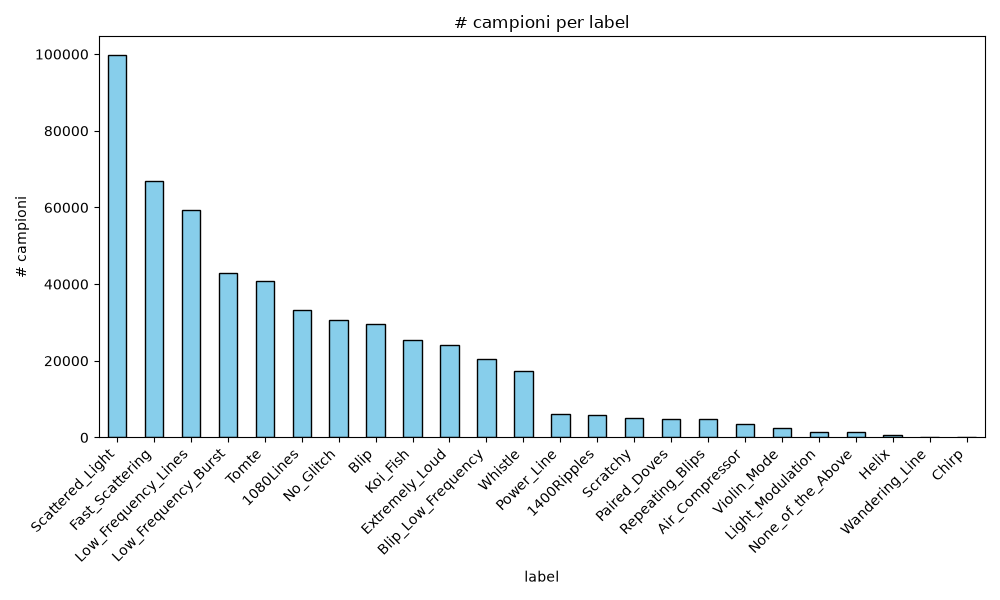
\includegraphics[width=0.75\linewidth]{label_counts.png}
\caption{Class frequencies in the Gravity Spy machine-learning release, all
observing runs and both detectors combined. The distribution is strongly
imbalanced; the four retained classes are among the most populated.}
\label{fig:label-counts}
\end{figure}

\emph{Morphological diversity.} The four span physically distinct families of
instrumental noise~\cite{zevin2017, glanzer2023, bahaadini2018}: short broadband
transients of teardrop morphology and $\sim$0.04\,s duration (Blip);
high-amplitude events that saturate the spectrogram (Extremely\_Loud);
long-duration arches of 2--2.5\,s correlated with ground motion, caused in O3 by
relative motion between the optical suspension and reaction-mass chains
(Scattered\_Light); and narrowband lines at $\sim$500\,Hz and harmonics,
corresponding to resonances of the glass fibres suspending the mirrors
(Violin\_Mode). Spanning the morphological range is what makes the explanation
analysis informative, since each class should elicit a recognizably different
attention pattern. An example of each is shown in
Figure~\ref{fig:examples}.

\begin{figure}[htbp]
\centering
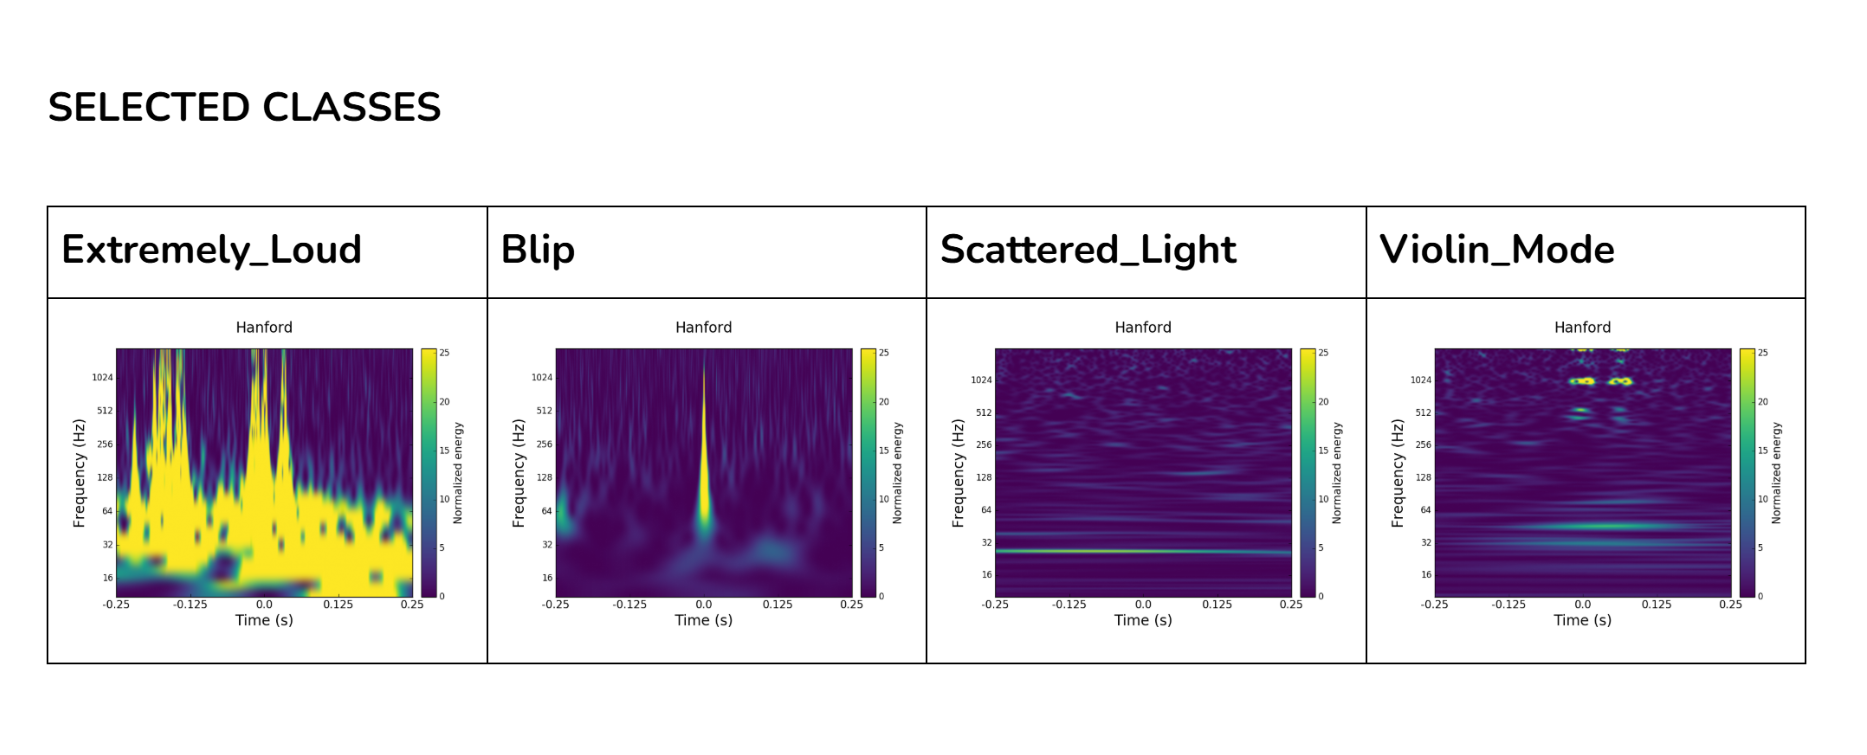
\includegraphics[width=\linewidth]{spectrogram_examples.png}
\caption{One Omega-scan spectrogram per retained class (Hanford detector, 0.5\,s
window). From left: a saturated broadband event, a short teardrop-shaped
transient, a long low-frequency band, and narrow lines near 500\,Hz and 1\,kHz.}
\label{fig:examples}
\end{figure}

\emph{Practical constraint.} Four classes keep training and the downstream
quantization grid feasible on a single 6\,GB consumer GPU.

Verification in the tabular domain shows each class isolated by a \emph{different}
descriptor, which is the relevant property: Extremely\_Loud occupies
$\log(\text{SNR}+1)$ between 6 and 12 while the others lie between 2 and 5; Blip
is separated by duration; Scattered\_Light sits below roughly 100\,Hz in peak
frequency with a bimodal bandwidth distribution; and Violin\_Mode is the only
class extending to 2\,kHz (Figure~\ref{fig:pairplot}). A UMAP
projection~\cite{mcinnes2018umap} of the standardized descriptors, computed on a
stratified subsample of 500 events per class ($n_\text{neighbors} = 15$,
seed 42), confirms the separation independently (Figure~\ref{fig:umap}).

\begin{figure}[htbp]
\centering
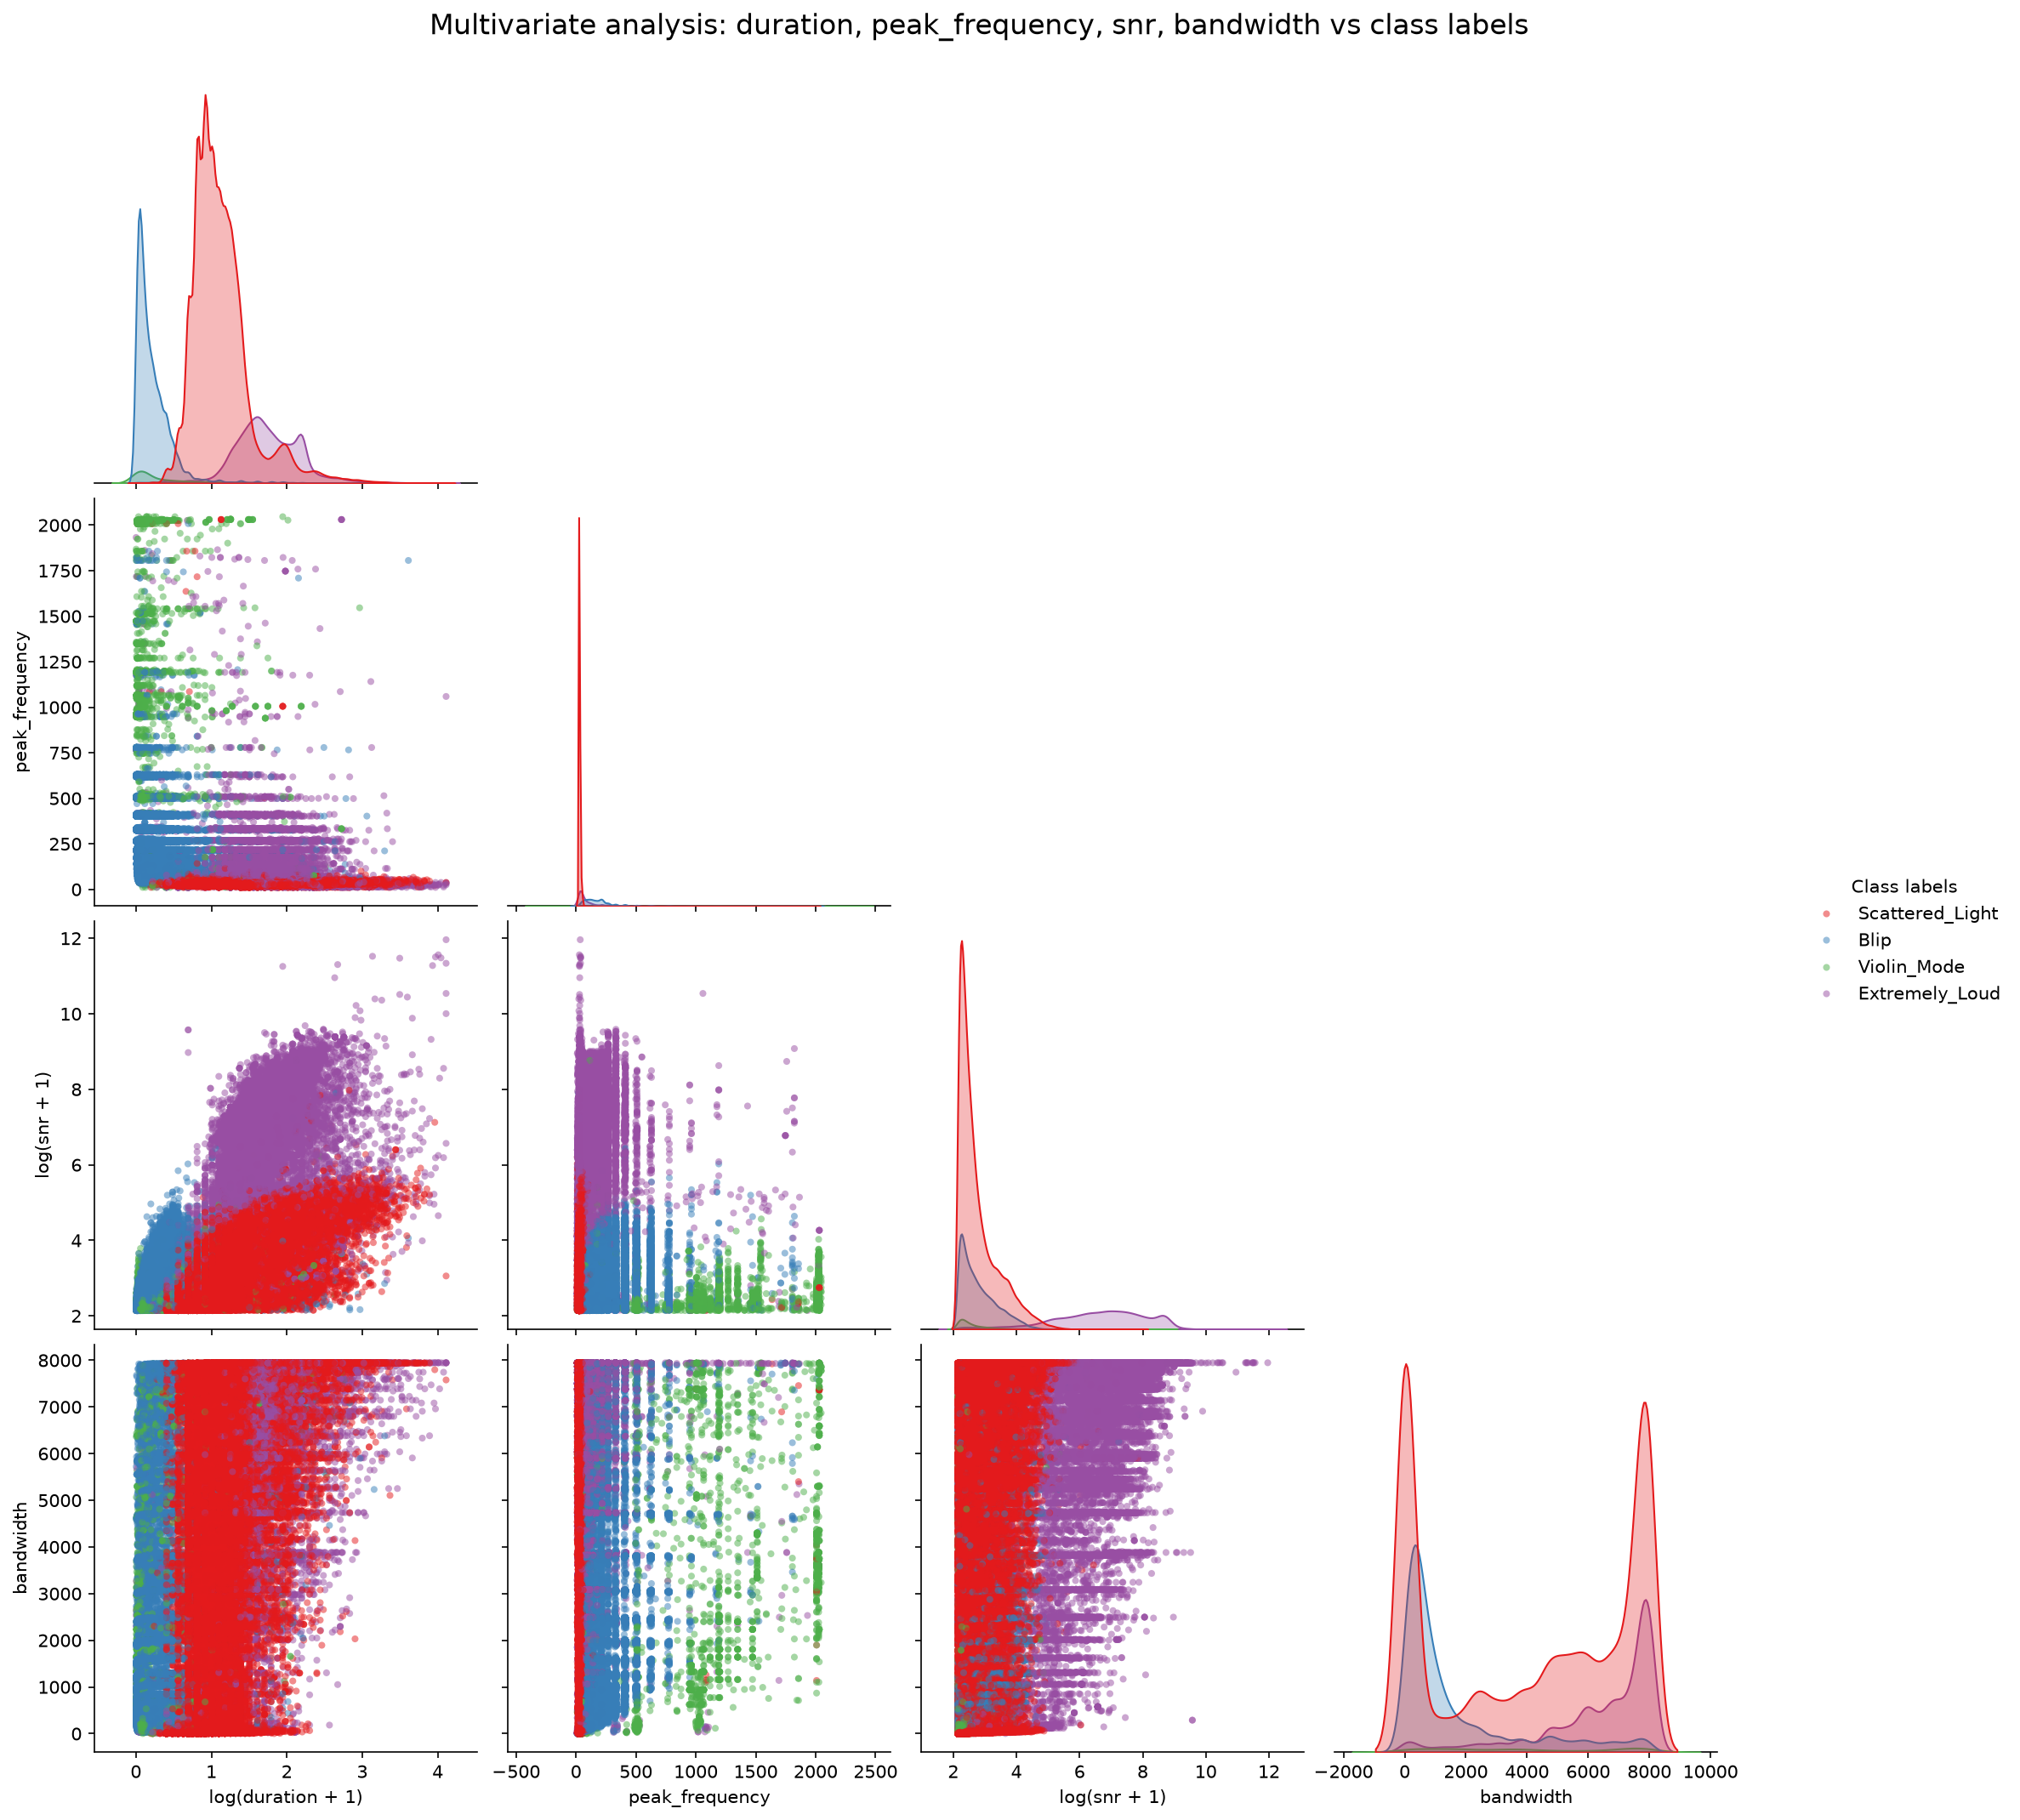
\includegraphics[width=0.85\linewidth]{pairplot.png}
\caption{Pair plot of the four retained descriptors, coloured by class. Each
class is isolated by a different descriptor; Violin\_Mode overlaps Blip and
Scattered\_Light except in peak frequency.}
\label{fig:pairplot}
\end{figure}

\begin{figure}[htbp]
\centering
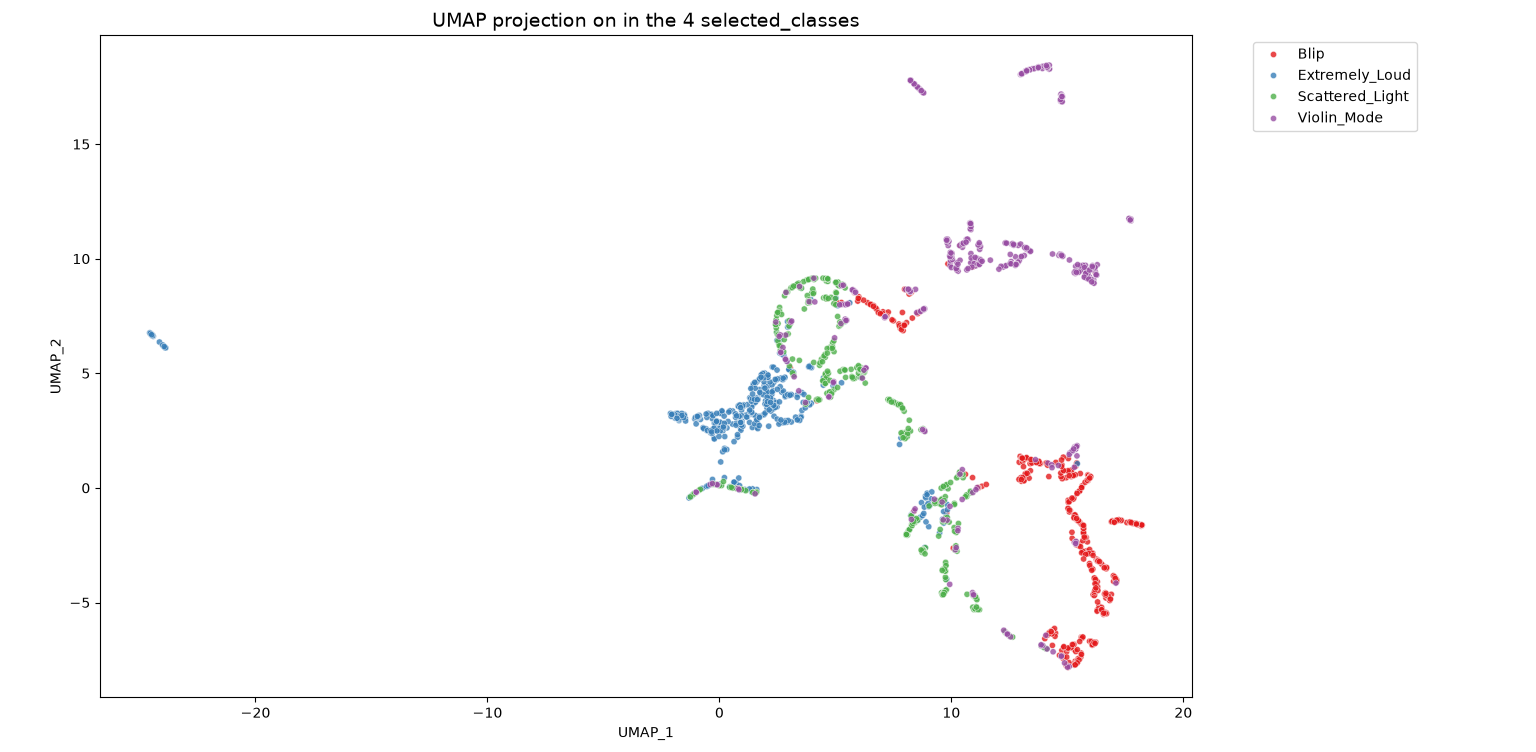
\includegraphics[width=0.85\linewidth]{umap.png}
\caption{Two-dimensional UMAP projection of the standardized descriptors, 500
events per class.}
\label{fig:umap}
\end{figure}

Violin\_Mode is the weakest case, and this is stated because it anticipates a
result that recurs throughout: in the $\log(\text{SNR}+1)$ versus
$\log(\text{duration}+1)$ plane it overlaps both Blip and Scattered\_Light, being
separated only in peak frequency. It is the lowest-recall class at every
configuration tested and the most sensitive class in every explainability
measurement.

Restricting the problem to four classes keeps it tractable, but means the results
are not directly comparable to the full Gravity Spy benchmark.

\subsection{Feature selection}

Of the twelve numerical Omicron descriptors, four were retained on three distinct
criteria, read from their distributions and from their correlation matrix
(Figure~\ref{fig:correlation}).

\begin{figure}[htbp]
\centering
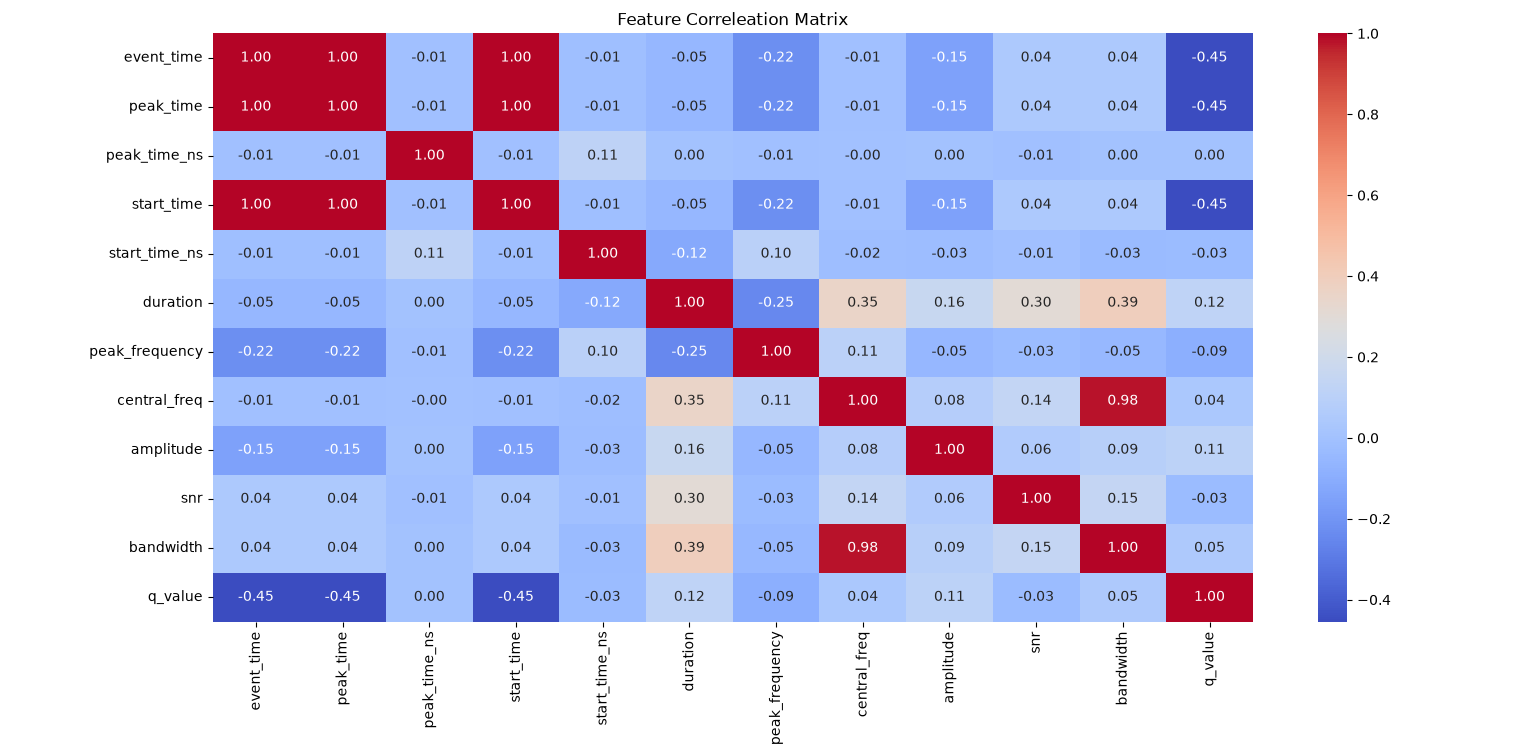
\includegraphics[width=0.9\linewidth]{correlation_matrix.png}
\caption{Pearson correlation between the twelve numerical Omicron descriptors.
The three timestamps are perfectly correlated, and central frequency and
bandwidth correlate at $0.98$.}
\label{fig:correlation}
\end{figure}

\emph{Exact redundancy.} The three timestamp variables are mutually correlated at
$r = 1.00$, being the same GPS time to within sub-second offsets. Beyond the
redundancy, retaining any of them would supply \emph{when} a glitch occurred
rather than \emph{what} it is, and the correlation matrix shows this is an
exploitable shortcut: event time correlates at $-0.45$ with the quality factor
and $-0.22$ with peak frequency, reflecting instrumental drift across observing
runs. Separately, central frequency and bandwidth correlate at $0.98$; bandwidth
was retained because peak frequency already encodes spectral position, so
bandwidth supplies extent rather than duplicating location.

\emph{Degenerate distributions.} The nanosecond remainders are uniformly
distributed and correlate with everything between $0.00$ and $0.11$, consistent
with timing quantization noise. The quality factor contains a sentinel value of
order $10^{20}$ that compresses the real distribution to the axis origin.

\emph{Normalized counterpart preferred.} Amplitude is a raw strain amplitude,
heavily skewed and dependent on the calibration and noise level at the time of
the trigger; SNR carries the same information normalized to the local noise floor
and is therefore comparable across detectors and epochs.

The four retained descriptors --- peak frequency, duration, bandwidth, SNR ---
form a complete and non-redundant characterization of a transient in the
time--frequency plane: spectral position, temporal extent, spectral extent and
prominence. Their largest pairwise correlation is $0.39$, well below the $0.98$
that forced the exclusion of central frequency.

Only one of the four image URL columns was kept. The four correspond to
successive time windows of the same detection (0.5\,s, 1\,s, 2\,s, 4\,s), and the
first was retained. Because they are \emph{different views} rather than
duplicates, they are not interchangeable, which is why unavailable images were
excluded rather than substituted from another column.

Residual class imbalance is removed by random undersampling to the cardinality of
the smallest class, giving an exactly balanced set of $9\,568$ images.

\subsection{Preprocessing and partition}

The downloaded spectrograms are matplotlib figures comprising a frame with axes,
colour bar and annotation. A centre crop of $470 \times 550$ pixels isolates the
spectrogram panel, which is then resized to the working resolution; the order
matters, since cropping the original and resizing afterwards keeps the same
portion of the spectrogram framed at every resolution. Channel-wise
normalization uses the standard ImageNet statistics, which also fixes the neutral
reference value used later by the deletion metric.

\textbf{The partition is frozen to disk.} A dedicated script generates the
train/validation/test assignment once, 70\,/\,15\,/\,15 under a fixed seed, and
writes it as a per-file record of path, class and split; every subsequent run
reads that file. A file listed but absent from disk is dropped from its partition
with a warning; a file present but unlisted raises, since an unassigned sample
would otherwise be used without anyone knowing where it belongs.

Freezing the partition rather than recomputing it gives two properties a seed
alone does not. Because the assignment is a function of the file list rather than
of the corpus size, removing a file removes exactly that file instead of
reshuffling every remaining assignment. And the audit trail is externally
verifiable: a reader can confirm that no file appears in two partitions, and the
manifest records the SHA-256 digest of the assignment file.

Four downloaded files proved unreadable. Two were recovered by re-downloading;
two are permanently unavailable at source (0.02\,\% of the corpus) and were
excluded. \textbf{Both belong to the training partition}, so the validation and
test sets are complete and identical to those on which the hyperparameters were
selected, which is why the search did not need to be repeated.

The final corpus is \textbf{9\,566 images, partitioned $6\,695 / 1\,435 /
1\,436$}. Beyond class balance, the three partitions are indistinguishable on the
physical properties of the events: median SNR is $14.97 / 14.09 / 14.98$, with
duration, peak frequency and bandwidth similarly matched.

\section{Model}

\subsection{Architecture}

\texttt{GWGlitchSNN} is a four-block convolutional spiking network. Each block is
a $5 \times 5$ convolution with stride 2 and padding 2 followed by a LIF layer;
spatial downsampling is performed by the stride rather than by pooling, which
keeps the spike tensors dense in time and avoids inserting a non-spiking operator
between layers.

\begin{table}[htbp]
\centering
\begin{tabular}{llll}
\toprule
Stage & Operation & Output shape & Notes \\
\midrule
Input & direct encoding $\times T$ & $[T, B, 3, 112, 112]$ & analog frame repeated \\
Block 1 & Conv $3\to16$, k5, s2, p2 + LIF & $[B, 16, 56, 56]$ & exposed as \texttt{spike1} \\
Block 2 & Conv $16\to32$, k5, s2, p2 + LIF & $[B, 32, 28, 28]$ & exposed as \texttt{spike2} \\
Block 3 & Conv $32\to64$, k5, s2, p2 + LIF & $[B, 64, 14, 14]$ & exposed as \texttt{spike3} \\
Block 4 & Conv $64\to128$, k5, s2, p2 + LIF & $[B, 128, 7, 7]$ & exposed as \texttt{spike4} \\
Readout & Flatten (6\,272) $\to$ Linear $\to$ LIF & $[B, 4]$ & one neuron per class \\
\bottomrule
\end{tabular}
\caption{Layer configuration at the working resolution of 112\,px. The flattened
width is derived from the input size at construction ($25\,088$ at 224\,px,
$6\,272$ at 112\,px, $2\,048$ at 64\,px), and the forward pass raises if the
input resolution does not match the one the model was built for.}
\label{tab:architecture}
\end{table}

The forward pass returns the stacked output spike train \emph{and} the four
hidden spike tensors of shape $[T, B, C, H, W]$, so that every diagnostic and
explainability procedure consumes raw hidden spike trains directly from the model
interface rather than through hooks.

Parameter count is nearly resolution-independent: $295\,332$ at 112\,px, of which
$270\,240$ are convolutional and unaffected by input size. Only the linear
readout shrinks with resolution, a fact with consequences for the design of the
quantization grid discussed in Section~\ref{sec:grid}.

Batch normalization, pooling and dropout are intentionally absent. Normalization
layers interact non-trivially with quantization, and their treatment belongs to a
later phase: batch normalization must be reconsidered for spiking networks in
general, quantizing its parameters is a problem distinct from quantizing weights
and potentials, and two alternative hardware strategies exist --- approximating
it with shifts, or eliminating it entirely.

\subsection{Readout and loss}

Classification uses a \emph{rate-coded readout}: output spikes are summed over
the $T$ time steps and the resulting per-class counts are passed to a
cross-entropy loss as logits. Optimization uses Adam~\cite{kingma2015adam}. This
keeps SAM in the multi-spike regime where its inter-spike-interval formulation
remains meaningful.

\section{Training}
\label{sec:training}

\subsection{Hyperparameter optimization}

Hyperparameters are searched with Optuna~\cite{akiba2019optuna}, maximizing
validation accuracy. Each trial reports validation accuracy after every epoch
and is pruned by a Hyperband pruner~\cite{li2018hyperband} (minimum resource 1
epoch, maximum 15, reduction factor 3), which allocates epochs to promising
configurations and truncates the others early. A handler catches out-of-memory
errors, releases the model and optimizer and marks the trial as pruned, so that
configurations with a long time window can fail on the 6\,GB budget of the
available GPU without interrupting the study. Studies are persisted to SQLite,
one study name per search and resolution.

Two studies were run. The first (v4), at 224\,px, searched the learning rate in
$[10^{-4}, 3 \times 10^{-3}]$ (log-uniform), $\beta$ in $(0, 1)$ and
$T \in \{5, \dots, 15\}$, and selected a learning rate of
$1.036 \times 10^{-4}$, $\beta = 0.4148$ and $T = 7$; this configuration was
used for the resolution study. The second (v5), at the working resolution,
imposes the deployment constraints described in
Section~\ref{sec:constrained-search} and produced the configuration used
throughout the rest of the thesis.

\subsection{Experiment tracking}

Every trial is logged to Weights \& Biases. Beyond validation loss and
accuracy, the logged metrics include the mean firing rate of each of the four
hidden layers. Firing rate is the proxy for energy consumption in spiking
hardware~\cite{roy2019towards}, so tracking it per layer during the search shows
whether high-accuracy configurations achieve their accuracy through dense and
expensive activity or through sparse spiking, and whether any layer is silent or
saturated before any explainability diagnostic is run.

A separately logged quantity, recorded under the name
\texttt{avg\_firing\_rate}, is the mean over the four \emph{output} neurons only.
A value near $0.25$ indicates that roughly one output neuron fires consistently,
which is a signature of confident classification rather than a measure of
network activity. It is \emph{not} the global firing rate of the network and is
never used for energy accounting, for which only the per-hidden-layer rates are
valid.

\subsection{Final training}

The training script reads the frozen configuration and trains from scratch,
parametrized on input resolution and seed, so that the same code serves the
resolution study, the final training and the multi-seed reference. The seed is
set explicitly before the model is constructed. The checkpoint is written
whenever validation accuracy improves, and training stops after five
consecutive epochs without improvement in validation loss, with a ceiling of 50
epochs. Each run writes the checkpoint together with a record of the full
per-epoch history, the per-layer firing rates, the per-class validation recall,
the seed and the resolution.

All experiments run on a single NVIDIA RTX 4050 Laptop GPU (6\,GB). One epoch
over the balanced training partition takes approximately three minutes at
224\,px and 45 seconds at 112\,px.

\section{Selecting the operating configuration}

Three choices define the operating point: the input resolution, the three
hyperparameters, and the decay constant of the explainer. Each is settled on
evidence and recorded in a single frozen manifest. Taking any of them on test-set
performance would consume the split reserved for the final estimate, so all three
are decided on validation.

\subsection{Input resolution}

Nine training runs were performed: three resolutions (224, 112, 64\,px) at three
seeds each, on the frozen partition, with hyperparameters held fixed and only the
input size varying. Since those hyperparameters had been found at 224\,px, the
protocol systematically handicaps the lower resolutions, and any deficit they
show is an upper bound.

The procedure and its outcome are reported in Section~\ref{sec:resolution}.

\subsection{Hyperparameter search under deployment constraints}
\label{sec:constrained-search}

The search uses Optuna~\cite{akiba2019optuna} with a Hyperband
pruner~\cite{li2018hyperband}, maximizing validation accuracy over three
hyperparameters chosen because they govern three distinct axes: learning rate
(optimization stability), $\beta$ (membrane leak and temporal memory), and $T$
(latency, computation and memory cost).

\textbf{Two deployment constraints are imposed inside the search space rather
than by rounding the result.} $\beta$ is restricted to
$\{0.25, 0.5, 0.75, 0.875\}$, values whose decay is realizable as a bit shift,
and the set spans both families ($\beta = 2^{-k}$ and $\beta = 1 - 2^{-k}$)
deliberately. $T$ is capped at 8 for the same reason. A rounded value is one that
was never validated; constraining the search guarantees that whatever it returns
is deployable by construction, and Section~\ref{sec:hyperparameters} shows that
in this case the two differ.

The lower bound of the learning rate was moved from $10^{-4}$ to $10^{-5}$,
because the v4 optimum ($1.036 \times 10^{-4}$) sat on the boundary of the
earlier range and a boundary optimum is not an optimum.

\subsection{Baseline manifest}

The outcome of these choices is recorded in a single file,
\texttt{baseline\_manifest.json}: the input resolution, the three
hyperparameters, the originating study, the decay rate and reference layer of
the explainer, the list of seeds (1234, 2345, 3456), the checkpoint paths, the
size of each partition, and the first sixteen hexadecimal digits of the SHA-256
digest of the partition file (\texttt{754b2515b6509075}). Every downstream
script reads the model and its configuration from the manifest rather than from
hard-coded paths, so that no analysis can silently run on a different model or a
different partition.

\section{Diagnostics of the network dynamics}
\label{sec:diagnostics}

Two diagnostics characterize whether a trained network is a healthy spiking
system or a formally correct one whose neurons are dead or saturated. Both are
reused unchanged on every quantized model.

\paragraph{Dead and saturated neurons.} For each hidden layer, the mean firing
rate of every individual neuron is accumulated across the validation partition,
weighted by batch size. A rate below $0.01$ identifies a \emph{dead} neuron,
above $0.80$ a \emph{saturated} one. Dead neurons are wasted capacity and, being
permanently silent, cannot appear in any explanation; saturated neurons carry
almost no information, a nearly-always-firing binary unit having minimal
entropy, while consuming the maximum possible energy.

\paragraph{Regularity of firing.} The coefficient of variation of the
inter-spike intervals,
\begin{equation}
\mathrm{CV} = \frac{\sigma_{\mathrm{ISI}}}{\mu_{\mathrm{ISI}}},
\end{equation}
distinguishes regular, clock-like firing ($\mathrm{CV} \to 0$) from irregular,
Poisson-like firing ($\mathrm{CV} \approx 1$). It is relevant here because the
Spike Activation Map is built on inter-spike intervals. A random sample of 200
neuron positions per layer is fixed once, at the first batch, and the intervals
of exactly those positions are accumulated over every validation image; the CV
is computed only where at least five intervals were observed. Since a neuron can
produce at most $T - 1 = 7$ intervals within a single image, pooling over the
whole partition is what makes the estimate stable.

\section{The Spike Activation Map}
\label{sec:sam-method}

SAM is implemented in two stages, following the original
formulation~\cite{kim2021sam}. The temporal spike contribution score weights a
past spike at $t'$ by its recency with respect to the current step $t$:
\begin{equation}
T(t, t') = \exp\left(-\gamma\,|t - t'|\right).
\end{equation}
The neuronal contribution score of a neuron at time $t$ sums that weight over the
neuron's preceding spikes, so a unit that has recently fired repeatedly --- one
with short inter-spike intervals --- receives a high score:
\begin{equation}
N^{k}_{ij,t} = \sum_{t' \in P^{k}_{ij},\; t' < t} T(t, t') .
\label{eq:ncs}
\end{equation}
The heat map at time $t$ masks that score with the spikes actually emitted at $t$
and sums over the channel axis, yielding one spatial map per time step:
\begin{equation}
M_{ij,t} = \sum_{k} N^{k}_{ij,t}\, S^{k}_{ij,t} .
\end{equation}

\paragraph{The summation range is exclusive of $t$.} This is stated explicitly
because an earlier implementation in this work summed over $t' \leq t$, and the
error is instructive. The score measures the contribution of a neuron's
\emph{preceding} trajectory; including $t' = t$ adds a term of weight
$\exp(0) = 1$ for every neuron firing at $t$, so the map produced is the correct
SAM \emph{plus the raw binary spike map}. The pedestal is independent of both
$\gamma$ and the spike history, and therefore inflates every correlation between
maps computed at different $\gamma$. A consequence of the correct definition is
that SAM at $t = 0$ is identically zero, no past history existing at the first
step.

The implementation uses the recursion
\begin{equation}
N_{t+1} = e^{-\gamma}\left(N_{t} + S_{t}\right), \qquad N_0 = 0,
\end{equation}
algebraically identical to Equation~\ref{eq:ncs} but $O(T)$ rather than
$O(T^2)$. A reference implementation computing the explicit sum is retained and
the two are asserted equal at run time.

Visualizations overlay every time step on the denormalized input under a
\emph{shared colour scale}, so that a change in intensity across time is genuine
and not an artefact of per-panel rescaling.

The reference configuration for every analysis below is \textbf{layer 2 with
$\gamma = 0.5$}, both recorded in the manifest. The choice of $\gamma$ is
justified in Section~\ref{sec:gamma}.

\section{Evaluating and comparing explanations}
\label{sec:xai-protocol}

\subsection{Multi-sample statistics}

A single heat map is a glimpse, not a description of what the network attends to
for a class. For each class, SAM is computed on 25 validation images, aggregated
over time (mean over $T$) and stacked, and three maps are reported: the
\emph{mean}, the region attended on average; the \emph{standard deviation},
where the explanation varies most across instances; and their ratio, the
\emph{coefficient of variation}, which indicates whether a region is attended
consistently or only in some examples. Mean and standard deviation share a
colour scale across classes so that they are numerically comparable; the
coefficient of variation has an extremely long tail where the mean is near zero,
and its colour scale is truncated at the 95th percentile.

The same statistics are repeated for all four hidden layers, on 20 images per
class. Since SAM sums over the channel axis and the four layers have 16, 32, 64
and 128 channels, raw magnitudes are not comparable across depth, and both maps
are normalized by the channel count of their layer before being plotted on a
shared scale.

\subsection{Faithfulness: the deletion metric}

Stability is not correctness, so faithfulness is tested separately with the
deletion metric of Petsiuk et al.~\cite{petsiuk2018rise}:
\begin{enumerate}
  \item the time-aggregated SAM map of an image is upsampled bilinearly from the
        layer resolution to the input resolution, so that importance is
        expressed over input pixels;
  \item the class predicted on the unmodified image is recorded and tracked
        throughout, since SAM is class-agnostic and the metric measures
        faithfulness to the model's decision;
  \item pixels are removed in decreasing order of SAM score, in 21 steps from
        0\,\% to 100\,\%, and the softmax confidence of the tracked class is
        recorded at each step;
  \item the identical procedure is repeated with pixels removed in random
        order, as a control;
  \item the curves are averaged over 15 images per class and compared through
        their area under the curve (AUC), computed by the trapezoidal rule.
\end{enumerate}
A faithful map degrades the confidence faster than random removal, so
$\Delta = \mathrm{AUC}_{\mathrm{SAM}} - \mathrm{AUC}_{\mathrm{random}} < 0$ is
the expected outcome. Deleted pixels are set to zero in normalized space, which
corresponds to the dataset mean rather than to black; the ordering is computed
once per image and sliced progressively, so that the removed sets are nested for
both curves.

\subsection{Divergence metrics}
\label{sec:metrics}

Two explanations of the same image, produced by two models, are compared with
three metrics, each answering a different question.

\paragraph{Spatial Pearson correlation (PCC).} The linear correlation between
the two time-aggregated maps, flattened. It is invariant to an affine rescaling
of either map, which is the property that makes it usable across models whose
overall spiking activity differs.

\paragraph{Top-$k$ intersection over union (IoU).} The overlap between the sets
of the $k = 20\,\%$ highest-scoring positions of the two maps. Two independent
random rankings overlap at a chance level of $k / (2 - k) = 0.111$.

\paragraph{Temporal centre of mass (CoM).} The mean time step at which the
energy of the SAM map is concentrated,
\begin{equation}
\mathrm{CoM} = \frac{\sum_t t \, E_t}{\sum_t E_t},
\qquad E_t = \sum_{i,j} M_{ij,t},
\end{equation}
reported as the absolute difference between the two models. Being an aggregate
over the whole map, it is the metric that carries the temporal axis.

In addition, the \emph{per-timestep correlation} between the maps at each $t$
localizes in time where agreement breaks down.

\subsection{Calibration protocol}
\label{sec:calibration-protocol}

The divergence metrics are calibrated before they are used, at three levels,
all on fifteen validation images per class at the reference layer and $\gamma$,
on the three checkpoints of the full-precision reference.

\begin{enumerate}
  \item \textbf{Verification.} A checkpoint compared with itself must return
        perfect agreement; two calls to the sampling routine must return
        bit-identical images; and two forward passes of the same model must
        return identical maps.
  \item \textbf{Independent solutions.} The three full-precision checkpoints are
        compared pairwise, which measures how similar two independently trained
        solutions are.
  \item \textbf{Numerical floor.} Gaussian noise is added to the weight tensors
        of one checkpoint, at magnitudes expressed as fractions of its measured
        8-bit quantization step, and the perturbed model is compared with the
        unperturbed one. Biases and the LIF buffers are excluded, since
        perturbing $\beta$ would mix membrane dynamics with weight noise.
\end{enumerate}
The $\gamma$ sensitivity analysis supplies a further reference point: the
divergence produced by changing the explainer itself thirtyfold.

\chapter{The Quantization Study}
\label{ch:quantization}

This chapter describes how the quantized models are built and how they are
compared with their full-precision parents. Every design choice below is either
inherited from the calibration of Section~\ref{sec:calibration} or settled by a
measurement reported in Section~\ref{sec:membrane-prep}; none is taken on the
test partition.

\section{Design principle: three separate arms}
\label{sec:grid}

The critical design choice is to \textbf{quantize the two targets separately
before quantizing them together}. Quantizing weights and membrane potential at
once would produce a single observation from which the contribution of each could
not be recovered; separating them turns the grid into a causal ablation and is
what makes the hypothesis of Chapter~\ref{ch:introduction} testable.

\begin{table}[htbp]
\centering
\resizebox{\linewidth}{!}{%
\begin{tabular}{llll}
\toprule
Arm & Weights & Membrane potential & Purpose \\
\midrule
FP32 reference & 32-bit float & 32-bit float & baseline for every comparison \\
Weight-only (W) & 8 / 4 / 2 bit & 32-bit float & isolates the synaptic (spatial) effect \\
Membrane-only (U) & 32-bit float & 8 / 4 / 2 bit & isolates the state (temporal) effect \\
Joint (W+U) & 8 / 4 / 2 bit & 8 / 4 / 2 bit & deployable configuration \\
\bottomrule
\end{tabular}}
\caption{The quantization grid: ten configurations, each at the three seeds of
the reference.}
\label{tab:grid}
\end{table}

Two quantities are deliberately left out of the grid. The membrane decay
$\beta = 0.75$ is already shift-implementable, having been constrained inside the
hyperparameter search (Section~\ref{sec:constrained-search}), and is not
re-quantized, which would be a third, unplanned intervention. The biases are kept
in full precision: there are 244 of them, under $0.1\,\%$ of the parameters,
and on integer hardware they are added once to a wide accumulator.

The two arms have \emph{opposite} sensitivities to the resolution choice, which
independently justifies treating them as separate ablations. Because $270\,240$
of the $295\,332$ parameters are convolutional and therefore
resolution-independent, the weight arm achieves nearly the same absolute memory
reduction at any resolution, whereas the membrane state falls twelvefold between
224 and 64 pixels.

\section{Quantization-aware training from the parent}
\label{sec:qat}

Quantization-aware training is implemented by fake quantization: in the forward
pass each quantized tensor is rounded to its grid and clamped to the grid's
bounds, and in the backward pass the rounding is replaced by the identity, the
straight-through estimator~\cite{bengio2013ste}.

\paragraph{Every quantized model is fine-tuned from the full-precision
checkpoint of the same seed.} This is the constraint that determines the rest of
the design. The numerical floor of the calibration ($\mathrm{PCC} = 0.975$) holds
for comparisons between a model and its own parent, where no channel permutation
exists; a quantized model trained from a random initialization would be an
independent solution, for which the relevant level is $0.153$ and almost no
quantization effect would be distinguishable from initialization variance. The
fine-tuning is therefore short and at reduced learning rate, adapting the parent
to its grid rather than finding a new solution. The relative $L_2$ distance
between the quantized weights and those of the parent is reported per layer, as
a check that each quantized model stayed in its parent's neighbourhood.

\todo{State the fine-tuning schedule actually used (number of epochs, learning
rate as a fraction of $1.047 \times 10^{-4}$, early-stopping rule) once fixed in
\texttt{train.py}.}

\paragraph{Execution order and sanity gate.} All 8-bit configurations are run
first, then 4-bit, then 2-bit. Before the grid is launched, the joint 8-bit model
of one seed must match its parent to within the spread of the full-precision
reference, four samples out of $1\,435$. At 8 bits the weight step is of the
order of the perturbation that left the spatial correlation at $0.975$ in the
calibration, so an appreciable loss of accuracy at that bit-width would indicate
a defect of the implementation, not a physical effect.

\paragraph{Fallback.} Should quantization-aware training prove unstable at the
lowest bit-widths, those configurations are produced by post-training
quantization of the parent instead, the procedure used by Rabbi et
al.~\cite{rabbi2026}; the comparison between the two procedures is then itself
reported.

\section{Weight quantizer}
\label{sec:weight-quantizer}

Weights are quantized on a \emph{symmetric signed} grid with
$q_{\max} = 2^{b-1} - 1$ levels on each side of zero, so that zero is exactly
representable: 255 levels at 8 bits, 15 at 4 bits and 3 at 2 bits (the values
$-\Delta, 0, +\Delta$, a ternary network). The quantizer is applied to every
convolutional and linear weight tensor, including the readout.

\textbf{The scale is computed per output channel.} The choice was made on the
measured weight distributions of the reference checkpoint
(Table~\ref{tab:weight-ranges}). In the deeper convolutions the largest weight
of the weakest channel is less than half the largest weight of the whole tensor,
so a per-tensor scale would leave that channel using fewer than half of the
levels: about one effective bit lost, which at 2 bits is the difference between
a ternary channel and a channel quantized entirely to zero.

\begin{table}[htbp]
\centering
\begin{tabular}{lcccc}
\toprule
Layer & $\max|w|$, tensor & $\max|w|$, weakest channel & Ratio & Bits lost per-tensor \\
\midrule
conv1  & 0.144 & 0.115 & 1.25 & 0.33 \\
conv2  & 0.126 & 0.060 & 2.11 & 1.08 \\
conv3  & 0.113 & 0.054 & 2.11 & 1.08 \\
conv4  & 0.099 & 0.044 & 2.26 & 1.18 \\
linear & 0.214 & 0.146 & 1.46 & 0.55 \\
\bottomrule
\end{tabular}
\caption{Weight ranges of the reference checkpoint (seed 1234). ``Bits lost'' is
$\log_2$ of the ratio: the resolution that the weakest channel would forgo under
a single per-tensor scale.}
\label{tab:weight-ranges}
\end{table}

The global 8-bit step used in the calibration ($0.00168$, from the largest
absolute weight of the network, $0.214$) is therefore an upper bound on the
per-channel steps actually applied.

\section{Membrane quantizer}
\label{sec:membrane-quantizer}

The membrane potential of the four hidden LIF layers is quantized at every time
step. The quantizer acts on the potential returned by each layer after the spike
decision, so the quantized value is the \emph{state} carried into the next step:
what is stored, and therefore what costs memory, is what is quantized. The
output layer, four neurons, is left in full precision; its state is negligible in
memory and quantizing it would act directly on the logits.

A grid for the membrane cannot be designed without knowing the range of the
quantity, and unlike a weight, the potential has no range until the network is
run. Its distribution was therefore measured over the whole validation partition
(Section~\ref{sec:membrane-prep}), and the clipping range was chosen by testing
candidate ranges on the full-precision network before any quantization.

\textbf{The membrane grid is unsigned over $[0, 2]$}, twice the firing threshold
$U_{\text{thr}} = 1$. The step is $2/(2^b - 1)$:

\begin{table}[htbp]
\centering
\begin{tabular}{cccc}
\toprule
Bits & Levels & Step & Step / threshold \\
\midrule
8 & 256 & 0.0078 & 0.8\,\% \\
4 & 16  & 0.1333 & 13.3\,\% \\
2 & 4   & 0.6667 & 66.7\,\% \\
\bottomrule
\end{tabular}
\caption{The membrane grid at each bit-width. At 2 bits the representable
potentials are $0$, $2/3$, $4/3$ and $2$: a single level lies strictly between
rest and threshold.}
\label{tab:membrane-grid}
\end{table}

Table~\ref{tab:membrane-grid} contains a quantitative prediction. At 8 bits the
rounding error is below one percent of the threshold; at 4 bits it is an eighth
of it; at 2 bits the error is of the same order as the threshold itself, and a
neuron's state can encode only whether it is at rest, below threshold, or above
it. This is the mechanism behind the observation of Smith et
al.~\cite{smith2026} that membrane quantization needs at least four bits, and the
grid tests it directly.

The unsigned scheme is a consequence of the clipping study rather than an
assumption: the network turns out to make no use of negative potentials, so a
signed grid would spend half of its levels on values that carry no information,
the equivalent of losing one bit at every bit-width.

\section{Joint arm}

The joint arm applies both quantizers at once, with the per-channel weight scales
of Section~\ref{sec:weight-quantizer} and the fixed membrane grid of
Section~\ref{sec:membrane-quantizer}, at the same bit-width.

\todo{Decide whether the joint arm keeps independent scales (as currently
implemented in \texttt{model/quantization.py}) or shares a single scale between
weights and membrane in the style of MINT~\cite{yin2024mint}, as stated in the
progress report. If scales stay independent, remove ``MINT-style'' everywhere
and justify the choice here; if shared, describe how the shared scale is set.}

\section{Reading the results}
\label{sec:reading}

For every quantized model, SAM maps are recomputed on the same fifteen validation
images per class and compared with those of \textbf{the full-precision parent of
the same seed}, using the metrics of Section~\ref{sec:metrics}: spatial PCC,
top-20\,\% IoU, the temporal centre of mass, and the per-timestep correlation
curve. Structural similarity~\cite{wang2004ssim} is added for comparability with
Rabbi et al.; unlike the other metrics it is not scale-invariant, and the maps
are normalized before it is computed.

Three further measurements characterize behaviour rather than explanations:
\begin{itemize}
  \item \textbf{cross-faithfulness}: the deletion metric applied to the quantized
        model with its \emph{own} map and with the map of its \emph{parent}. The
        second is the operational question, since in practice one is tempted to
        explain a deployed model with the maps of the original;
  \item the \textbf{Earth Mover's Distance} between the per-neuron firing-rate
        distributions of quantized model and parent, for direct comparison with
        Smith et al.~\cite{smith2026};
  \item the \textbf{diagnostics} of Section~\ref{sec:diagnostics} --- dead and
        saturated fractions, CV-ISI --- since quantization can induce dead or
        saturated neurons, which is a candidate mechanism for \emph{why} an
        explanation changes.
\end{itemize}

Five rules, all established in Chapter~\ref{ch:results} before the grid was
run, govern how those numbers are read.

\begin{enumerate}
  \item \textbf{Below the numerical floor is noise.} A divergence smaller than
        that produced by weight noise of one 8-bit step ($\mathrm{PCC}$ $0.975$,
        IoU $0.704$, CoM difference $0.029$ steps) is not a result.
  \item \textbf{IoU is an early indicator, PCC a graded measure.} IoU has a
        dynamic range of $2.6\times$ its floor and saturates early; PCC has
        $34\times$.
  \item \textbf{Everything is reported per class.} The sensitivity ordering
        Violin\_Mode $>$ Scattered\_Light $>$ Blip $>$ Extremely\_Loud recurs
        under every intervention tested, so a pooled figure would average a class
        that responds strongly with one that does not respond at all.
  \item \textbf{A flat result on Extremely\_Loud is uninformative.} That class
        did not register any perturbation tested; absence of effect and inability
        to detect one cannot be told apart.
  \item \textbf{Cross-faithfulness is interpretable on Blip and Extremely\_Loud
        only}, the two classes on which the deletion metric separates SAM from a
        random baseline. On the other two there is no signal for quantization to
        degrade.
\end{enumerate}

\paragraph{The test of the hypothesis.} The hypothesis predicts an
\emph{ordering}: the membrane arm should displace the temporal centre of mass
beyond its floor at a higher bit-width than the one at which the weight arm
lowers the spatial correlation beyond its floor. The reverse order refutes it.

\section{Stratified analysis}
\label{sec:stratified-method}

An aggregate divergence per configuration admits only a yes-or-no answer.
Joining the per-sample outputs to the physical descriptors allows the result to
be reported as a relation instead.

The hypothesis is that divergence increases as event strength decreases, with a
mechanism specific to spiking networks: quantizing the membrane potential flips a
neuron's spike decision only where the potential lies within the quantization
error of the threshold, and weak events produce potentials that sit close to
threshold rather than overshooting it. Because a flipped spike is a discrete
event that propagates both to the next layer and forward in time through the
decay and reset, and because SAM is constructed from spike trains, the flip
changes the object the explanation is made of rather than merely perturbing it.

The prediction discriminates between arms: membrane quantization applies a fixed
absolute error and should show a steep dependence on event strength, whereas
weight quantization perturbs the input current approximately in proportion to the
signal and should be flatter.

Two preconditions were verified. SNR does translate into image intensity, the
Gravity Spy colour scale being fixed rather than auto-scaled per image. And SNR
is very nearly a proxy for class --- the top global SNR quartile is 92.8\,\%
Extremely\_Loud --- so stratification uses \textbf{terciles computed within each
class}, or any trend measured would be a class effect wearing a strength label.

Finally, the \emph{disagreement subset} --- validation images classified
correctly by the parent and incorrectly after quantization --- is characterized
by its physical descriptors, to ask whether quantization fails on a particular
kind of event.

\section{Energy and memory}
\label{sec:energy-method}

Synaptic operations are counted per layer as
\begin{equation}
\mathrm{SOP}_{\ell} = f_{\ell-1} \cdot T \cdot \mathrm{MAC}_{\ell},
\end{equation}
where $f_{\ell-1}$ is the mean firing rate of the preceding hidden layer and
$\mathrm{MAC}_{\ell}$ the multiply-accumulate count of the equivalent dense
layer, and multiplied by the per-operation costs of~\cite{horowitz2014}. The
rates are the per-hidden-layer figures measured on the converged checkpoint of
each configuration, never the output-layer quantity logged as
\texttt{avg\_firing\_rate}.

\textbf{One layer is asymmetric.} Under direct encoding the first convolution
receives analog pixel values rather than spikes, so its operations are
multiply-accumulates. Because the input is identical at every time step, the
current it produces is constant in time and is computed once rather than $T$
times. This is a standard implementation of constant encoding, but stating it
matters: recomputing that layer at every step would make the spiking network
more expensive than its convolutional equivalent (Section~\ref{sec:energy-fp32}).

Memory is the number of bits needed to store the weights plus those needed to
store the membrane state of the $94\,080$ hidden neurons at the working
resolution. For integer configurations the 8-bit energy figures of Horowitz are
used; at 4 and 2 bits they are a conservative upper bound, since narrower
operations are not tabulated.

\section{Test-set evaluation}

The test partition is opened once, after every design decision has been taken,
on the full-precision reference and on the quantized configurations selected for
the final comparison. Accuracy is reported with a 95\,\% Wilson interval and per
class, and is computed by two routes --- an aggregate over batches and a
per-sample classification --- asserted equal, since the per-sample output feeds
the stratified analysis.

\chapter{Results}
\label{ch:results}

\section{Input resolution}
\label{sec:resolution}

\subsection{Accuracy does not discriminate}

\begin{table}[htbp]
\centering
\begin{tabular}{lcccc}
\toprule
Input size & Val.\ accuracy & Std.\ dev. & Observed range & Epochs \\
\midrule
224\,px & 0.9854 & 0.0007 & 0.9847--0.9861 & 22.7 \\
112\,px & 0.9800 & 0.0035 & 0.9777--0.9840 & 17.3 \\
64\,px  & 0.9814 & 0.0011 & 0.9805--0.9826 & 24.7 \\
\bottomrule
\end{tabular}
\caption{Validation accuracy by input resolution, mean and standard deviation
over three seeds.}
\label{tab:resolution-accuracy}
\end{table}

The ordering in Table~\ref{tab:resolution-accuracy} is not monotonic --- 64\,px
outperforms 112\,px --- and a genuine resolution effect would produce monotonic
degradation. The arithmetic agrees: $0.9854$ corresponds to $21.0$ errors out of
$1\,435$ validation samples and $0.9814$ to $26.6$, a gap of $5.6$ samples,
against a 95\,\% Wilson interval on a single measurement of $\pm 0.7$ percentage
points. The four classes survive an elevenfold reduction in pixel count,
consistent with their being distinguished by coarse morphology rather than fine
texture.

Per-class recall is directional but small. Violin\_Mode degrades most from
224\,px to 64\,px, by $1.00$ percentage points, which is the direction predicted
from morphology since narrow spectral lines are the structure most vulnerable to
downsampling --- but the magnitude is $3.6$ samples out of $365$, inside the
confidence interval of a single measurement. Extremely\_Loud degrades more at
112\,px than at 64\,px, a second non-monotonicity. \textbf{No class collapses at
reduced resolution.}

\subsection{Network health does discriminate}

Since accuracy is uninformative, the resolution was decided on the internal state
of the network. For each hidden layer, the mean firing rate of every individual
neuron is accumulated across the validation partition. A rate below $0.01$
identifies a \emph{dead} neuron, above $0.80$ a \emph{saturated} one. Both are
pathological in different ways: dead neurons represent wasted capacity and,
being permanently silent, cannot appear in any explanation; saturated neurons
carry almost no information, a nearly-always-firing binary unit having minimal
entropy, while consuming the maximum possible energy.

\begin{table}[htbp]
\centering
\begin{tabular}{lcccc}
\toprule
Input size & Layer 1 & Layer 2 & Layer 3 & Layer 4 \\
\midrule
224\,px & $12.1 \pm 3.3$ & $16.6 \pm 4.9$ & $12.6 \pm 2.3$ & $\mathbf{36.3 \pm 4.0}$ \\
112\,px & $17.8 \pm 3.4$ & $11.8 \pm 0.8$ & $13.0 \pm 1.0$ & $\mathbf{23.6 \pm 2.9}$ \\
64\,px  & $16.4 \pm 4.8$ & $11.2 \pm 2.3$ & $11.7 \pm 2.3$ & $\mathbf{19.5 \pm 1.5}$ \\
\bottomrule
\end{tabular}
\caption{Percentage of dead neurons by layer and resolution, mean $\pm$ standard
deviation over three seeds, on validation.}
\label{tab:dead}
\end{table}

Layer 4 is the only layer that responds to resolution, and it responds on two
measures at once: the dead fraction falls monotonically from $36.3$\,\% to
$19.5$\,\%, while the median per-neuron firing rate rises from $0.0399$ to
$0.1499$. These were the two competing explanations for the higher mean activity
observed at lower resolution --- more neurons participating, or the same neurons
firing harder --- and both occur. Saturation does not increase to compensate:
neurons above $0.80$ remain below $2.5$\,\% in layer 4 at every resolution.

\textbf{The interpretation is spatial redundancy, not a cured pathology.} Layer 4
contains $25\,088$ neurons at 224\,px and $6\,272$ at 112\,px, so in absolute
terms the number of \emph{live} neurons falls from roughly $15\,970$ to $4\,789$.
Reducing the resolution does not increase usable capacity; it reduces capacity
while preferentially discarding units that were contributing nothing. At 224\,px
the deepest layer views a $14 \times 14$ map derived from a largely empty
spectrogram, and a third of its units never encounter signal.

\subsection{Decision: 112 pixels}

Most of the benefit comes from the first halving: 224 to 112\,px recovers $12.7$
percentage points of dead fraction, the further move to 64\,px only $4.1$ more.
Membrane state at 8 bits falls from 368\,KiB to 92\,KiB, bringing the full
inference state within the SRAM budget of the target class of devices.

The decisive argument against 64\,px is the spatial resolution of the
explanations themselves. SAM maps are computed on layer activations, whose side
lengths are 56, 28, 14 and 7 at 112\,px but 32, 16, 8 and 4 at 64\,px. A
$4 \times 4$ map contains sixteen values, on which centre-of-mass, top-$K$
intersection-over-union and structural similarity are all meaningless. Since the
contribution of this thesis is the fidelity of explanations rather than of
predictions, a configuration in which the measured object is degenerate in one
layer cannot be accepted whatever it saves in compute.

\section{Hyperparameters and the full-precision reference}
\label{sec:hyperparameters}

The constrained search selected \textbf{$\beta = 0.75$, $T = 8$, learning rate
$1.047 \times 10^{-4}$} at a best validation accuracy of $0.9847$ within the
15-epoch budget.

\textbf{The constraint on $\beta$ is justified empirically, not only by
argument.} An unconstrained search over $\beta \in (0,1)$ selects $0.4148$, whose
nearest admissible neighbours are $0.25$ and $0.5$. The constrained search
selects $0.75$. Rounding the unconstrained optimum after the fact --- the
alternative to constraining the space --- would therefore have produced a
configuration that is both inferior and never validated.

All four values were sampled; the search allocated 40\,\% of trials to $0.75$ and
10\,\% to $0.875$, which is itself the surrogate model's judgement after early
exploration. Among trials surviving at least three epochs, $0.75$ leads on both
the best ($0.9847$) and the median ($0.9763$) validation accuracy, while $0.875$
trails on both and was pruned in all three of its trials.

\textbf{$T = 8$ is an optimum at the imposed ceiling} and is reported as such:
the search was forbidden from exploring $T > 8$. The mitigating evidence is that
an unconstrained search with range up to 15 selected $T = 7$, so the preference
for long integration windows is mild.

\subsection{$\beta$ improves the measurement instrument}

Holding resolution and partition fixed and changing only $\beta$ from $0.4148$ to
$0.75$, the layer-4 dead fraction is \emph{unchanged} at $23.6$\,\%. $\beta$ does
not affect the dead fraction; resolution does. This strengthens the reading of
Section~\ref{sec:resolution}: the deep-layer problem is spatial redundancy rather
than a dynamical pathology curable by a better decay constant.

What $\beta$ does change is saturation, by an order of magnitude and most where
it matters. Neurons above $0.80$ fall from $9.3 / 3.5 / 2.7 / 1.8$\,\% across the
four layers to $4.7 / 0.22 / 0.06 / 0.14$\,\%. The layer-2 figure is the
consequential one, because a saturated neuron accumulates the maximum possible
contribution score on every image and therefore contributes a constant,
non-discriminative floor to every SAM map. \textbf{Selecting $\beta$ on
validation accuracy alone happened to reduce that contamination by a factor of
sixteen at the reference layer.}

\subsection{Three-seed reference}

\begin{table}[htbp]
\centering
\begin{tabular}{lcc}
\toprule
Quantity & Mean & Std \\
\midrule
Validation accuracy & 0.9833 & 0.0014 \\
Epochs to early stop & 21.0 & 1.7 \\
Recall, Blip & 0.9915 & 0.0028 \\
Recall, Extremely\_Loud & 0.9855 & 0.0000 \\
Recall, Scattered\_Light & 0.9839 & 0.0027 \\
Recall, Violin\_Mode & 0.9726 & 0.0099 \\
\bottomrule
\end{tabular}
\caption{Full-precision reference at 112\,px, $\beta = 0.75$, $T = 8$, over three
seeds on validation.}
\label{tab:fp32}
\end{table}

The reference is statistically indistinguishable from the 224\,px configuration
($0.9854$): three samples out of $1\,435$ separate them, against a four-sample
spread across seeds. \textbf{Reducing the pixel count by a factor of four, and
constraining $\beta$ and $T$ to hardware-realizable values, costs no measurable
accuracy.}

\textbf{Accuracy is reproducible; internal dynamics are not.} At fixed accuracy
the mean firing rate of layer 1 varies by a factor of $2.6$ across seeds, and the
coefficient of variation falls monotonically with depth: $46.9$\,\% at layer 1,
$28.6$\,\% at layer 2, $15.3$\,\% at layer 3, $9.5$\,\% at layer 4. The regime is
established within the first epoch and persists, indicating that initialization
selects the firing regime and training does not subsequently equalize it. A
measurement taken during the resolution study puts the effect in the units of
the closest work: the Wasserstein-1 distance between the per-layer firing-rate
profiles of two full-precision models differing only in seed is $0.039$, inside
the range of Earth Mover's Distances that Smith et al.~\cite{smith2026} report
\emph{between full-precision and quantized} models. This is the observation that
motivates Section~\ref{sec:calibration}.

\section{Physical validation of the dynamics}
\label{sec:physical}

At the adopted configuration the confusion matrix diagonal reads
$0.99 / 0.99 / 0.98 / 0.97$, consistent with Table~\ref{tab:fp32}; the only
non-negligible errors are on Violin\_Mode, the class that in the tabular domain
partially overlaps both Blip and Scattered\_Light (Figure~\ref{fig:confusion}).

\begin{figure}[htbp]
\centering
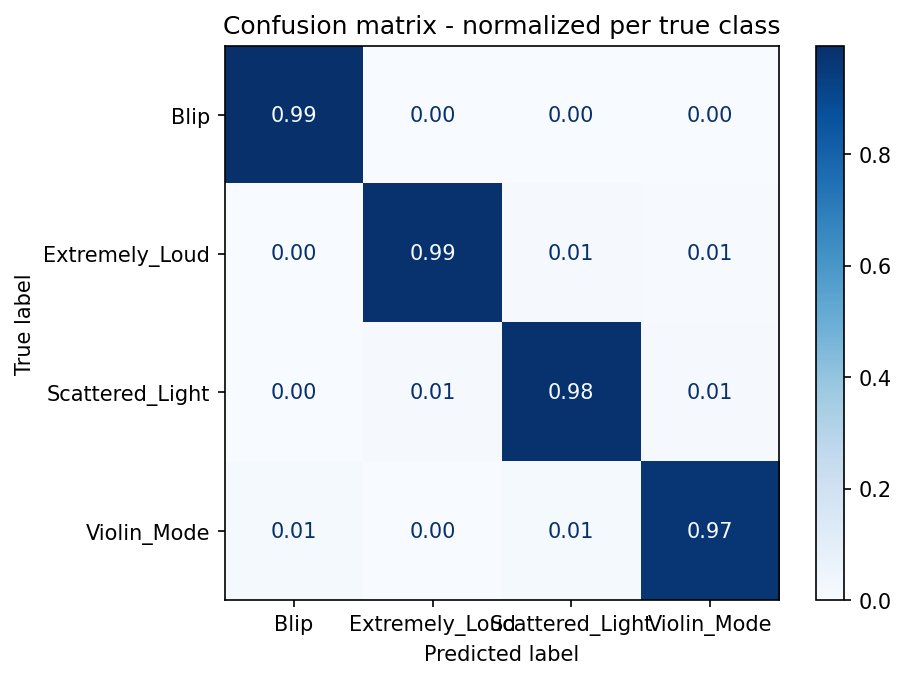
\includegraphics[width=0.6\linewidth]{confusion_matrix.png}
\caption{Confusion matrix of the reference checkpoint (seed 1234) on validation,
normalized per true class.}
\label{fig:confusion}
\end{figure}

The dead fraction is $16.1 / 12.6 / 11.3 / 22.8$\,\% across the four layers, and
\textbf{no neuron in any layer exceeds the saturation threshold}, a consequence
of $\beta = 0.75$ (Figure~\ref{fig:firing}). These figures reproduce those of Section~\ref{sec:resolution}
exactly for the same seed, computed through an independent code path, which is a
free verification of both.

One feature deserves note: the layer-1 distribution is \textbf{bimodal}, with a
secondary population near a firing rate of $0.65$--$0.75$ that has no counterpart
in the deeper layers. A high-activity subpopulation therefore exists in the first
layer only, which may be related to its being the layer with the largest
coefficient of variation across seeds.

\begin{figure}[htbp]
\centering
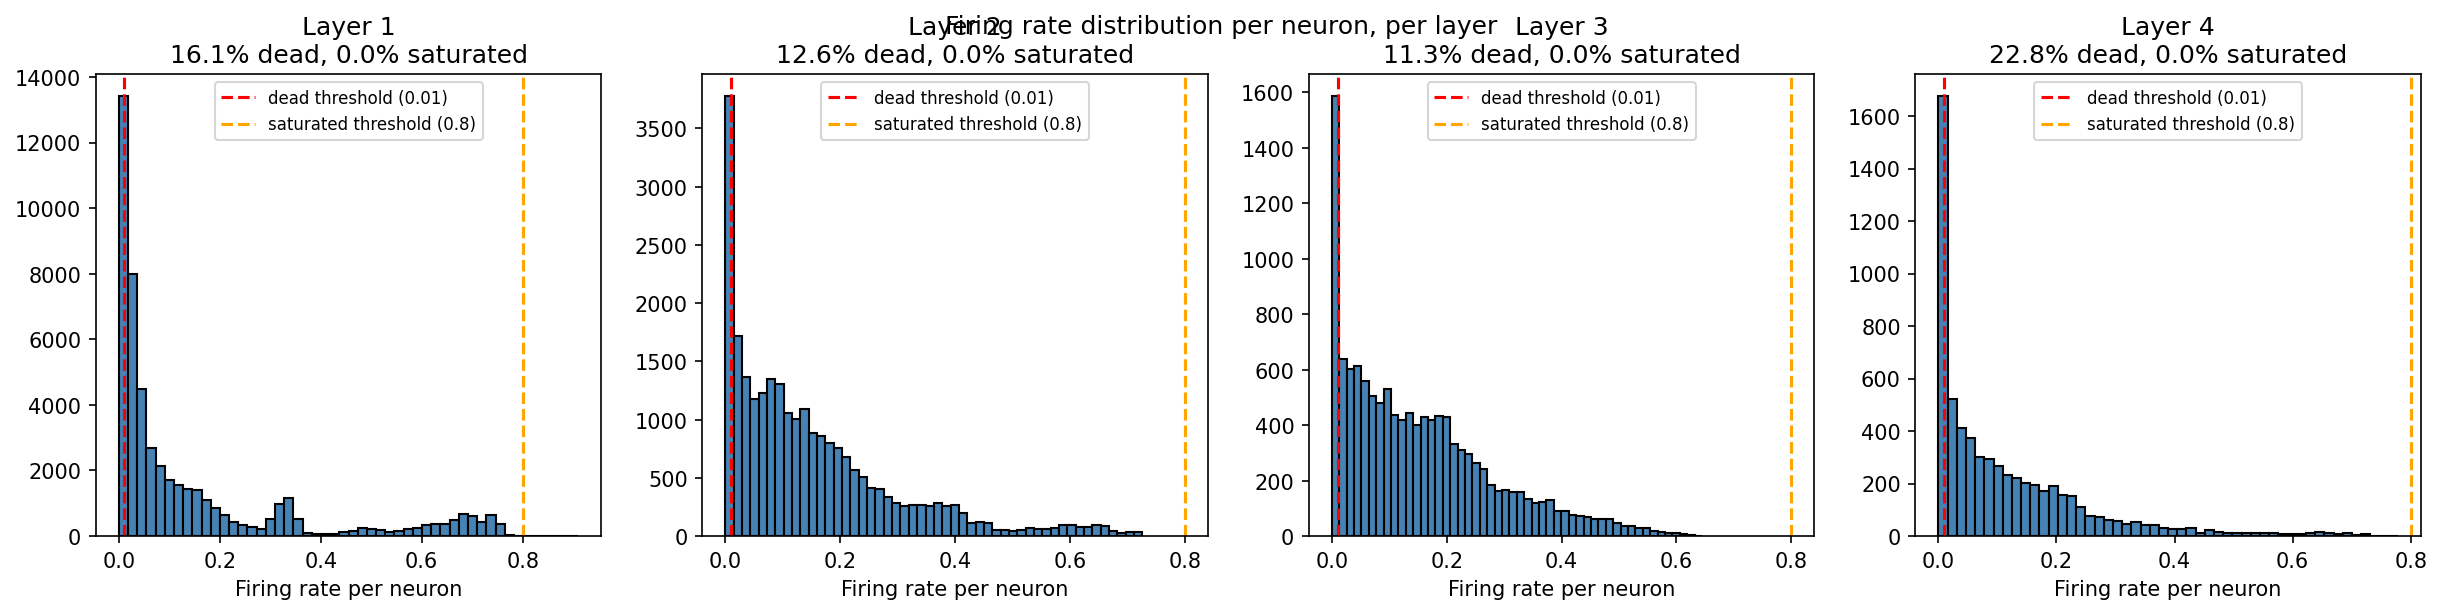
\includegraphics[width=\linewidth]{firing_rate_distributions.png}
\caption{Distribution of per-neuron firing rates in the four hidden layers, on
validation, with the dead ($0.01$) and saturation ($0.80$) thresholds.}
\label{fig:firing}
\end{figure}

The coefficient of variation of inter-spike intervals concentrates between $0.35$
and $0.45$ in all four layers. Firing is regular rather than Poisson-like, which
is the expected outcome under constant direct encoding: since the input does not
vary over time, any irregularity observed is generated entirely by the membrane
dynamics and by interaction between layers. This is evidence about internal
dynamics, not a claim of biological realism. With $T = 8$ a neuron can produce at
most seven intervals, so the five-interval threshold used for the estimate is
close to the ceiling, which is why the accumulation runs over the whole partition
rather than a single image. Between 184 and 196 of the 200 sampled neurons per
layer met the threshold (Figure~\ref{fig:cvisi}).

\begin{figure}[htbp]
\centering
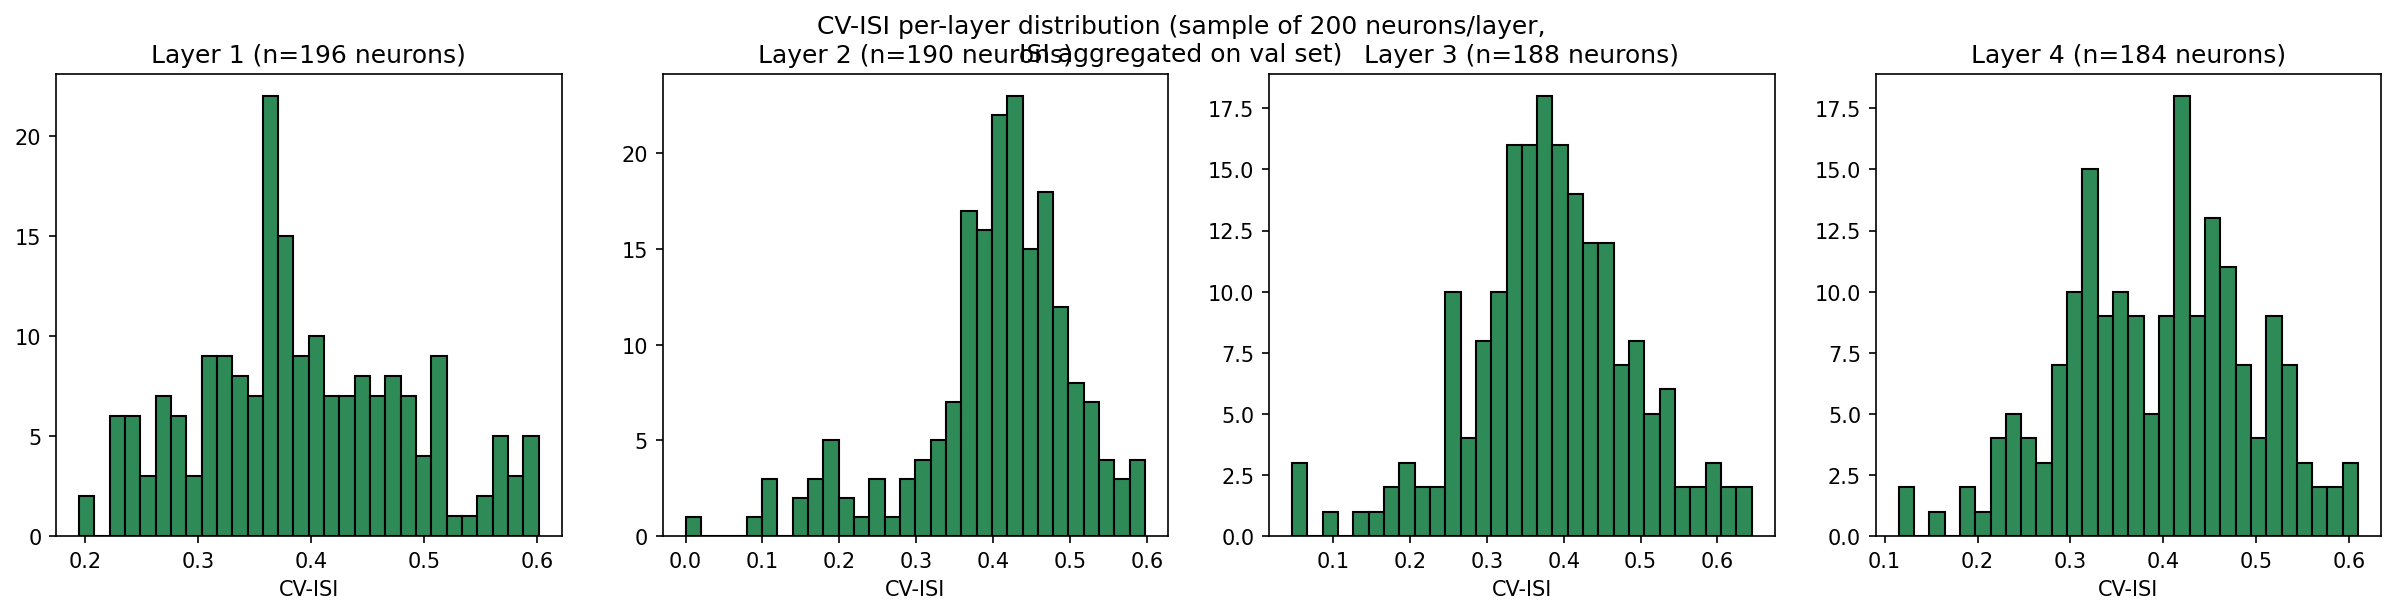
\includegraphics[width=\linewidth]{cv_isi_distributions.png}
\caption{CV of inter-spike intervals for 200 sampled neurons per layer,
accumulated over the validation partition.}
\label{fig:cvisi}
\end{figure}

\section{What the explanations show}
\label{sec:sam-results}

Figure~\ref{fig:sam-steps} shows the SAM sequence of a single Blip at the
reference layer. The map is zero at $t = 0$ by definition and builds up over
the first steps as spike histories accumulate; from the third step onward the
attended region is the vertical stroke of the glitch.

\begin{figure}[htbp]
\centering
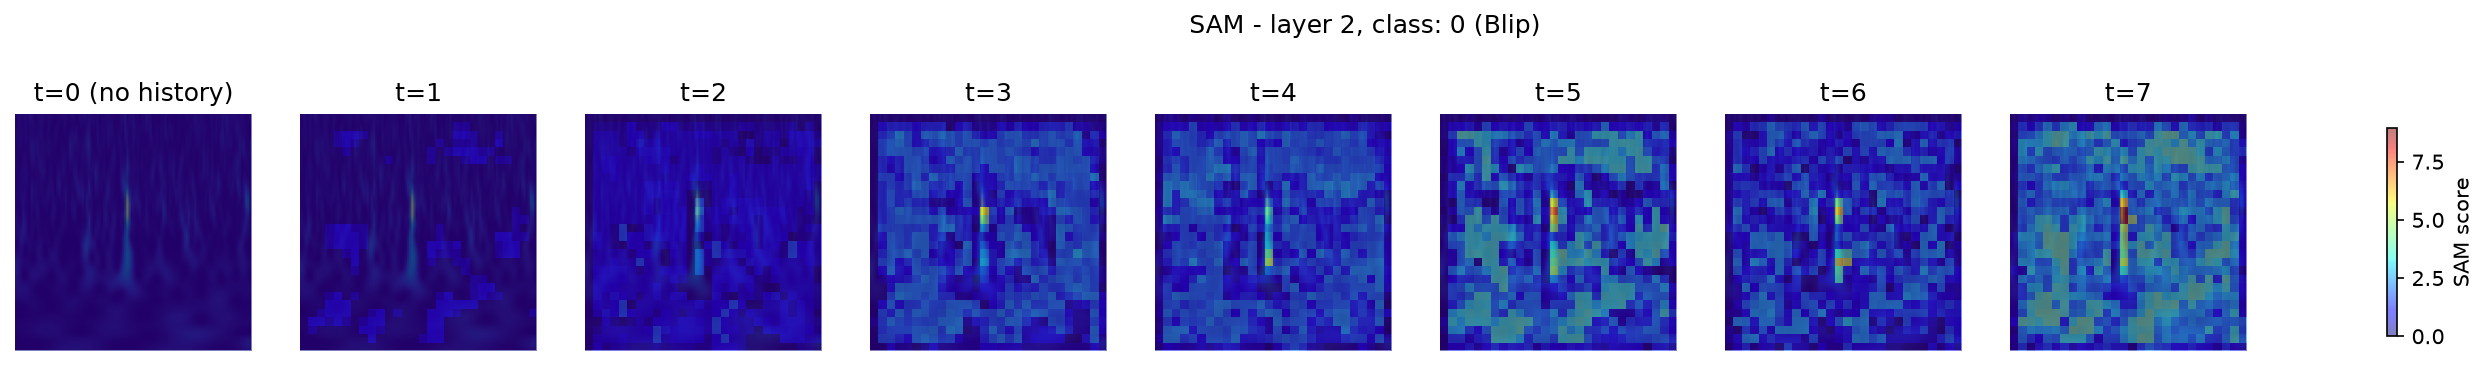
\includegraphics[width=\linewidth]{sam_visualization.png}
\caption{SAM at layer 2 for one Blip, one panel per time step, on a shared
colour scale.}
\label{fig:sam-steps}
\end{figure}

The class statistics (Figure~\ref{fig:sam-class}) show four recognizably
different attention patterns, each matching the morphology of its class. For
Blip the mean map concentrates on the narrow vertical stroke and so does the
variability, which is the stroke shifting slightly between instances. For
Extremely\_Loud the attended region is large and saturated, covering the lower
and central part of the spectrogram. For Scattered\_Light the attention lies on
a horizontal band at low frequency. Violin\_Mode produces the weakest and most
diffuse mean map, with variability concentrated in a few localized spots along
the line structure; it is also the class with the lowest recall, and the one
whose explanations prove most sensitive in every test below.

\begin{figure}[htbp]
\centering
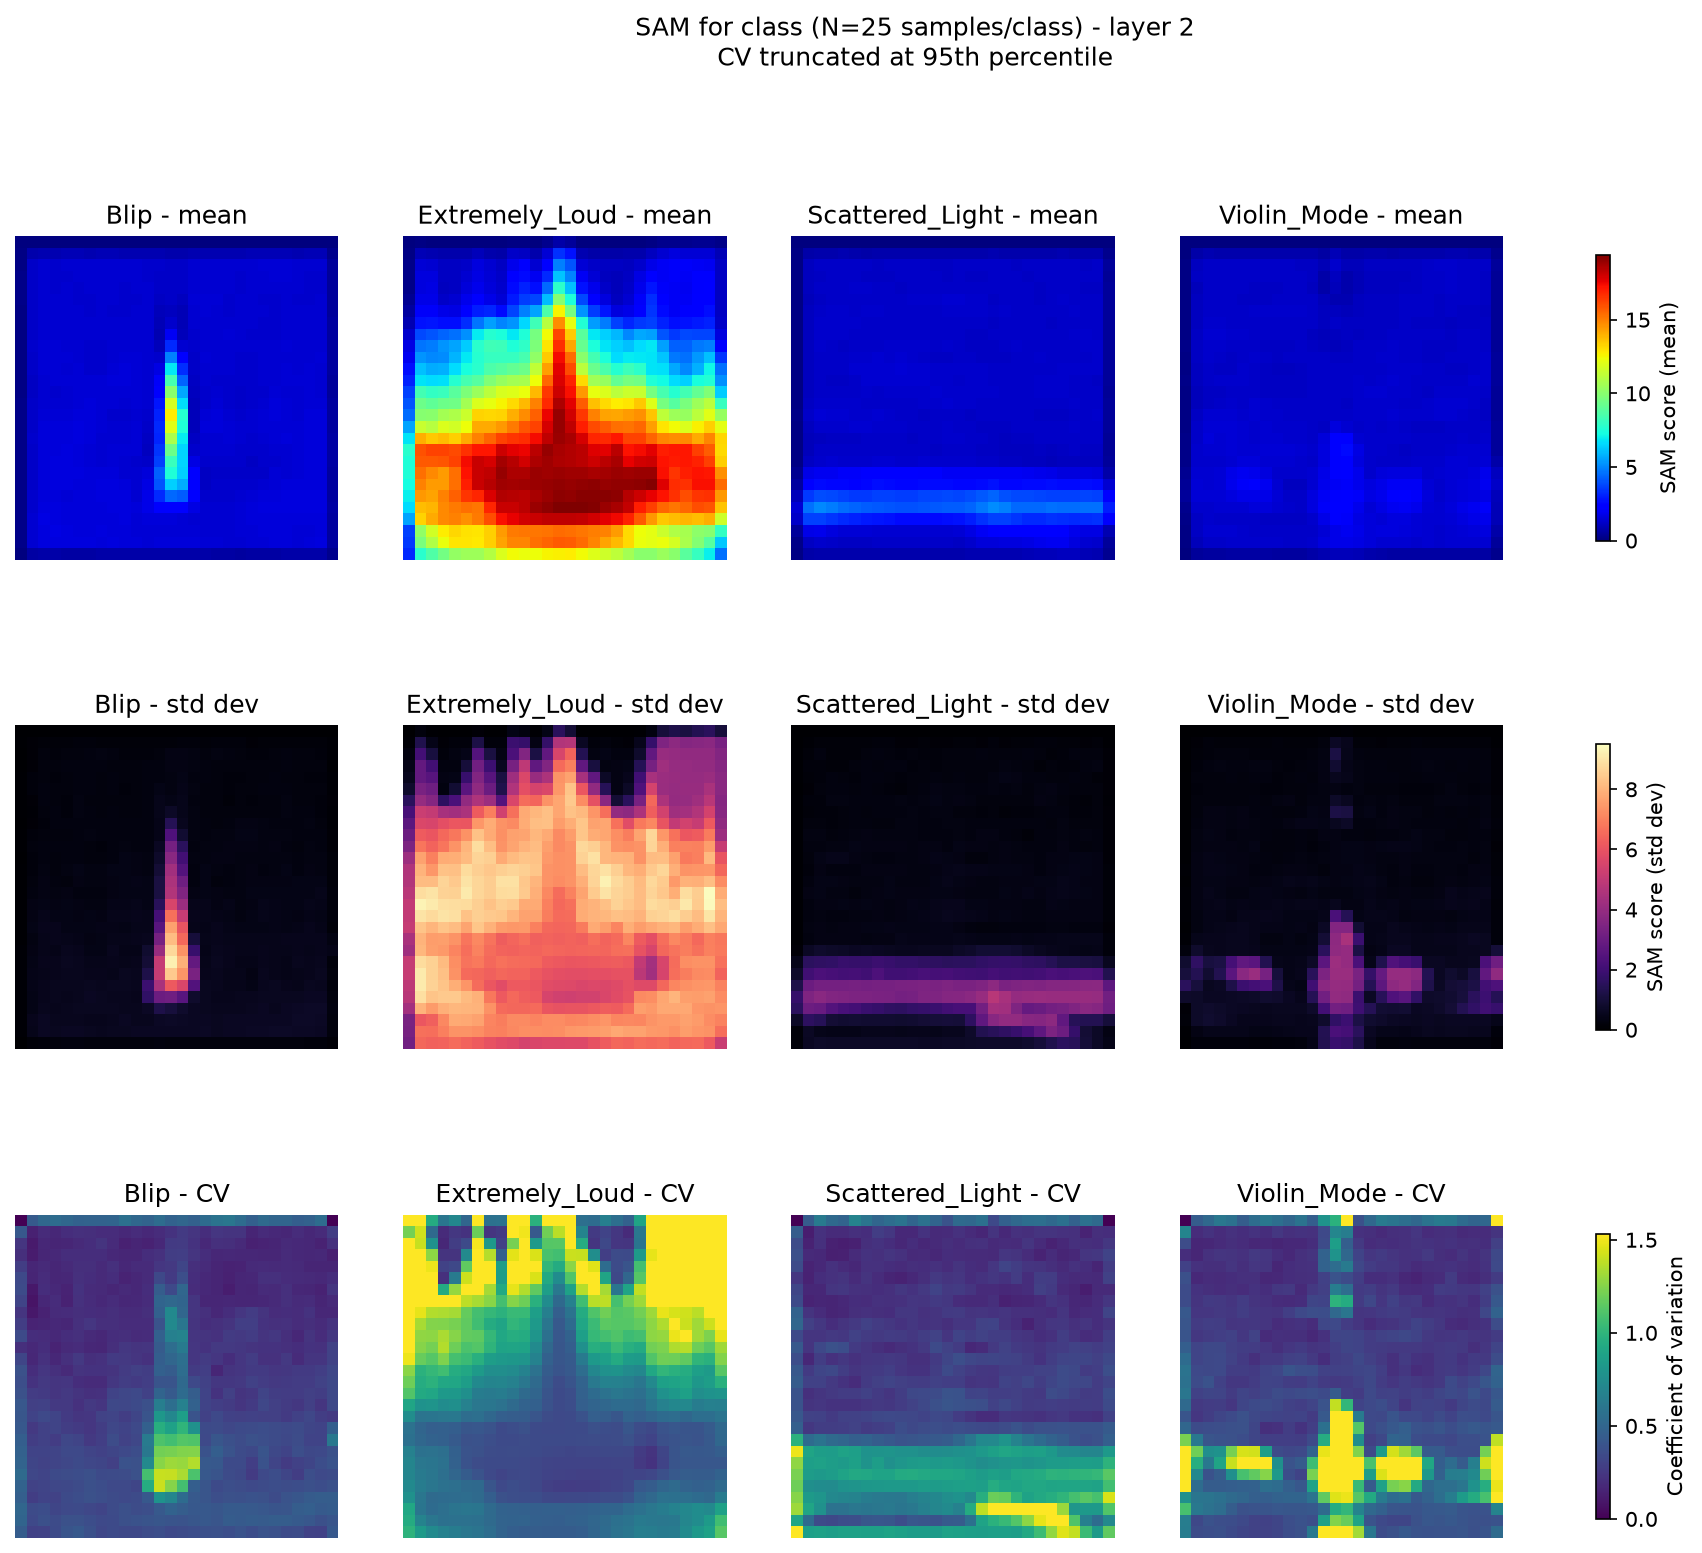
\includegraphics[width=0.9\linewidth]{sam_class_stats.png}
\caption{SAM statistics per class at layer 2, 25 validation images per class:
mean (top), standard deviation (middle) and coefficient of variation (bottom,
truncated at the 95th percentile). Mean and standard deviation share a colour
scale across classes.}
\label{fig:sam-class}
\end{figure}

Across depth (Figure~\ref{fig:sam-layers}) the progression is the expected one,
from fine localization in the early layers to coarse localization in the deep
ones, with maps of side 56, 28, 14 and 7. At layer 4 a $7 \times 7$ map leaves
only 49 positions, too few for a top-20\,\% overlap or a structural comparison
to be meaningful, while layer 2 still resolves the morphology of every class.

\todo{Confirm (or replace) this as the reason for choosing layer 2 as the
reference layer; the progress report records the choice but not its
justification.}

\begin{figure}[htbp]
\centering
\begin{subfigure}{0.49\linewidth}
  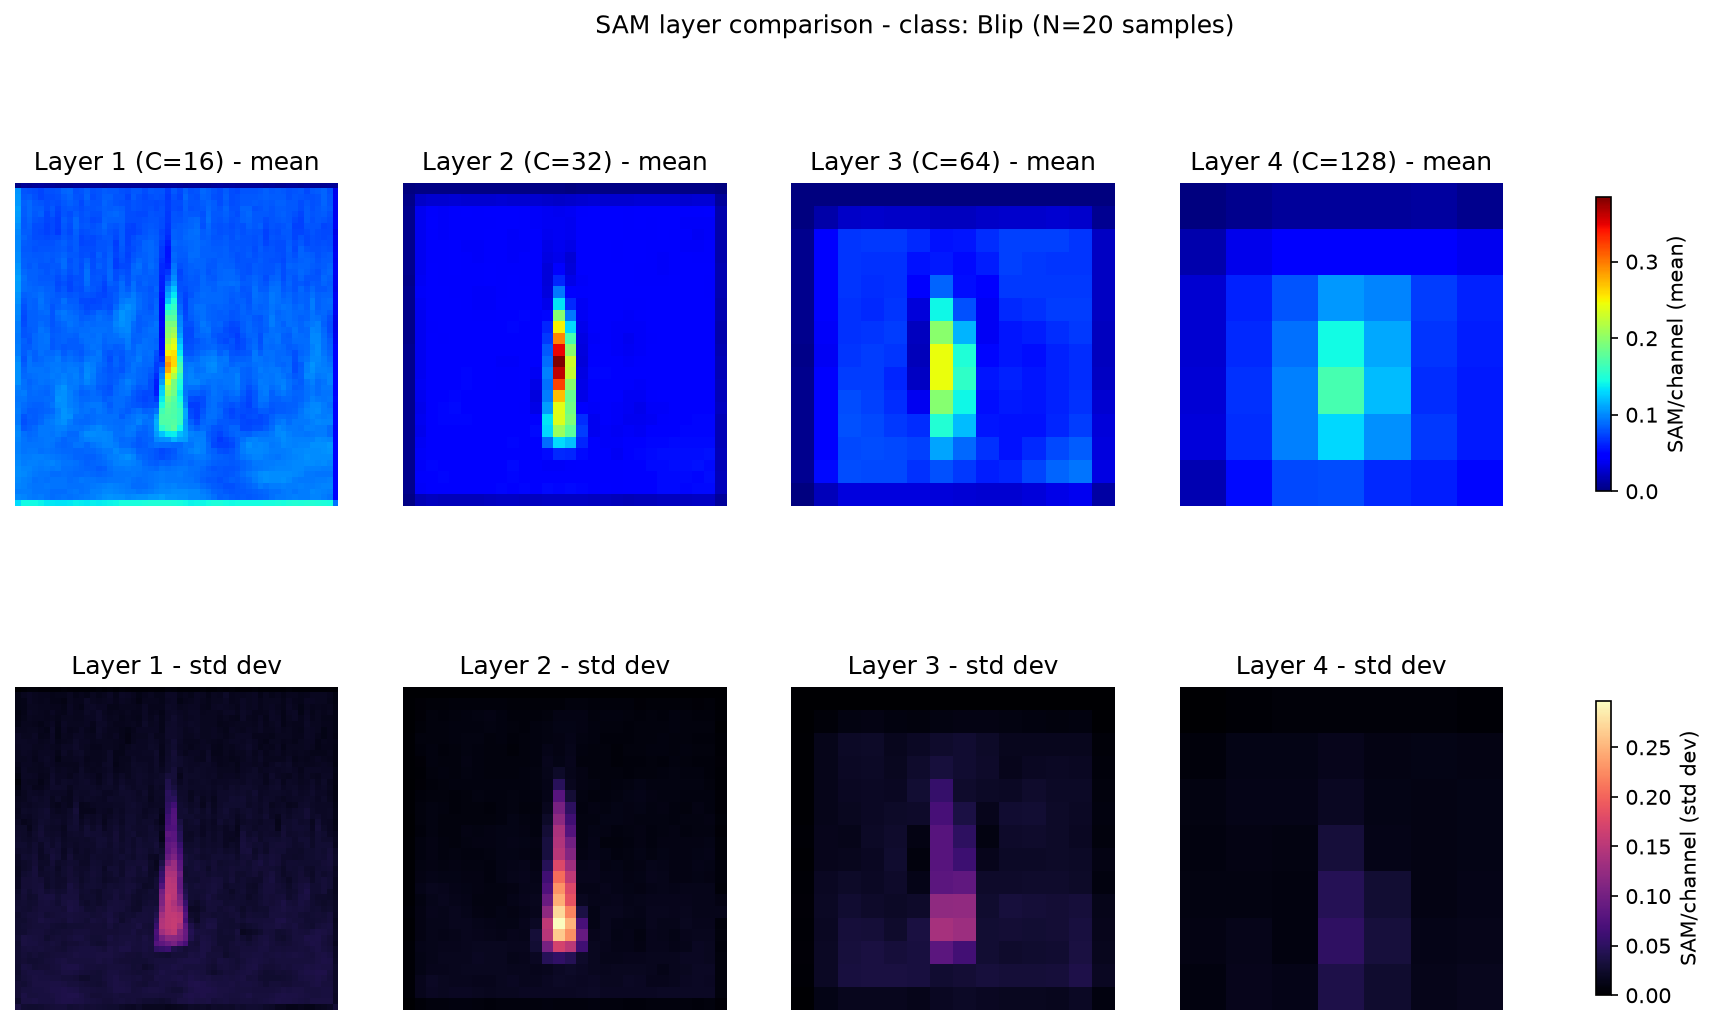
\includegraphics[width=\linewidth]{sam_layer_Blip.png}
  \caption{Blip}
\end{subfigure}\hfill
\begin{subfigure}{0.49\linewidth}
  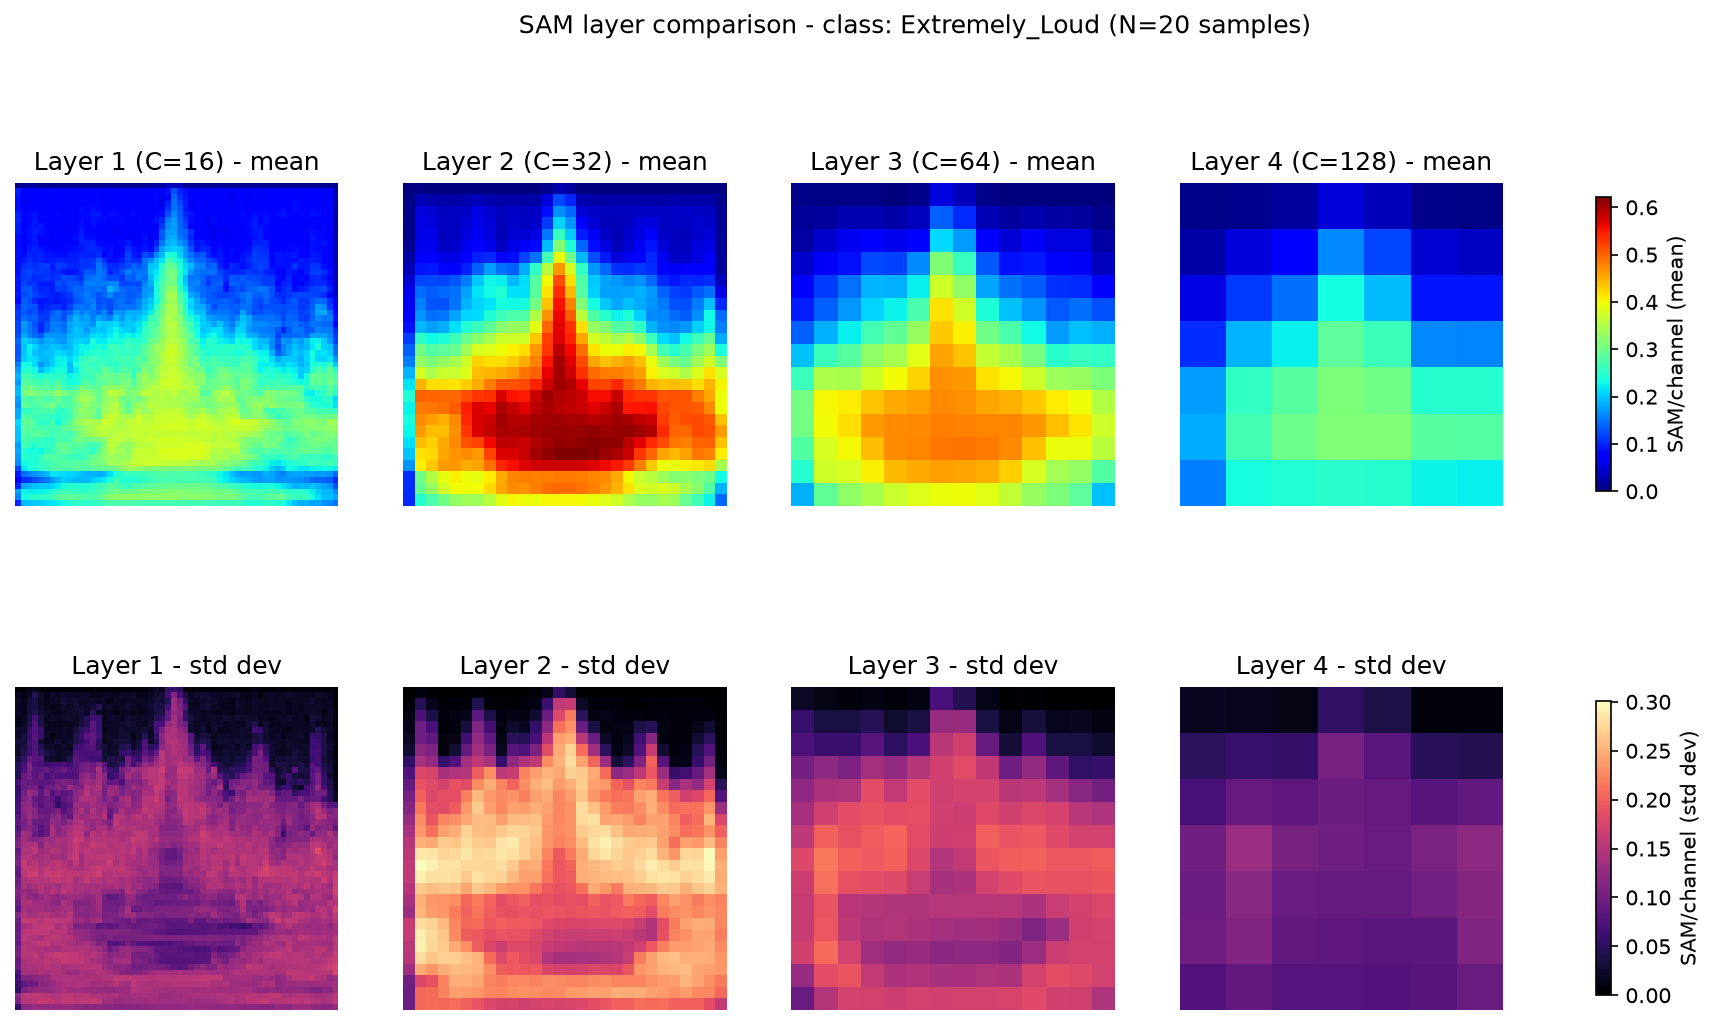
\includegraphics[width=\linewidth]{sam_layer_Extremely_Loud.png}
  \caption{Extremely\_Loud}
\end{subfigure}

\begin{subfigure}{0.49\linewidth}
  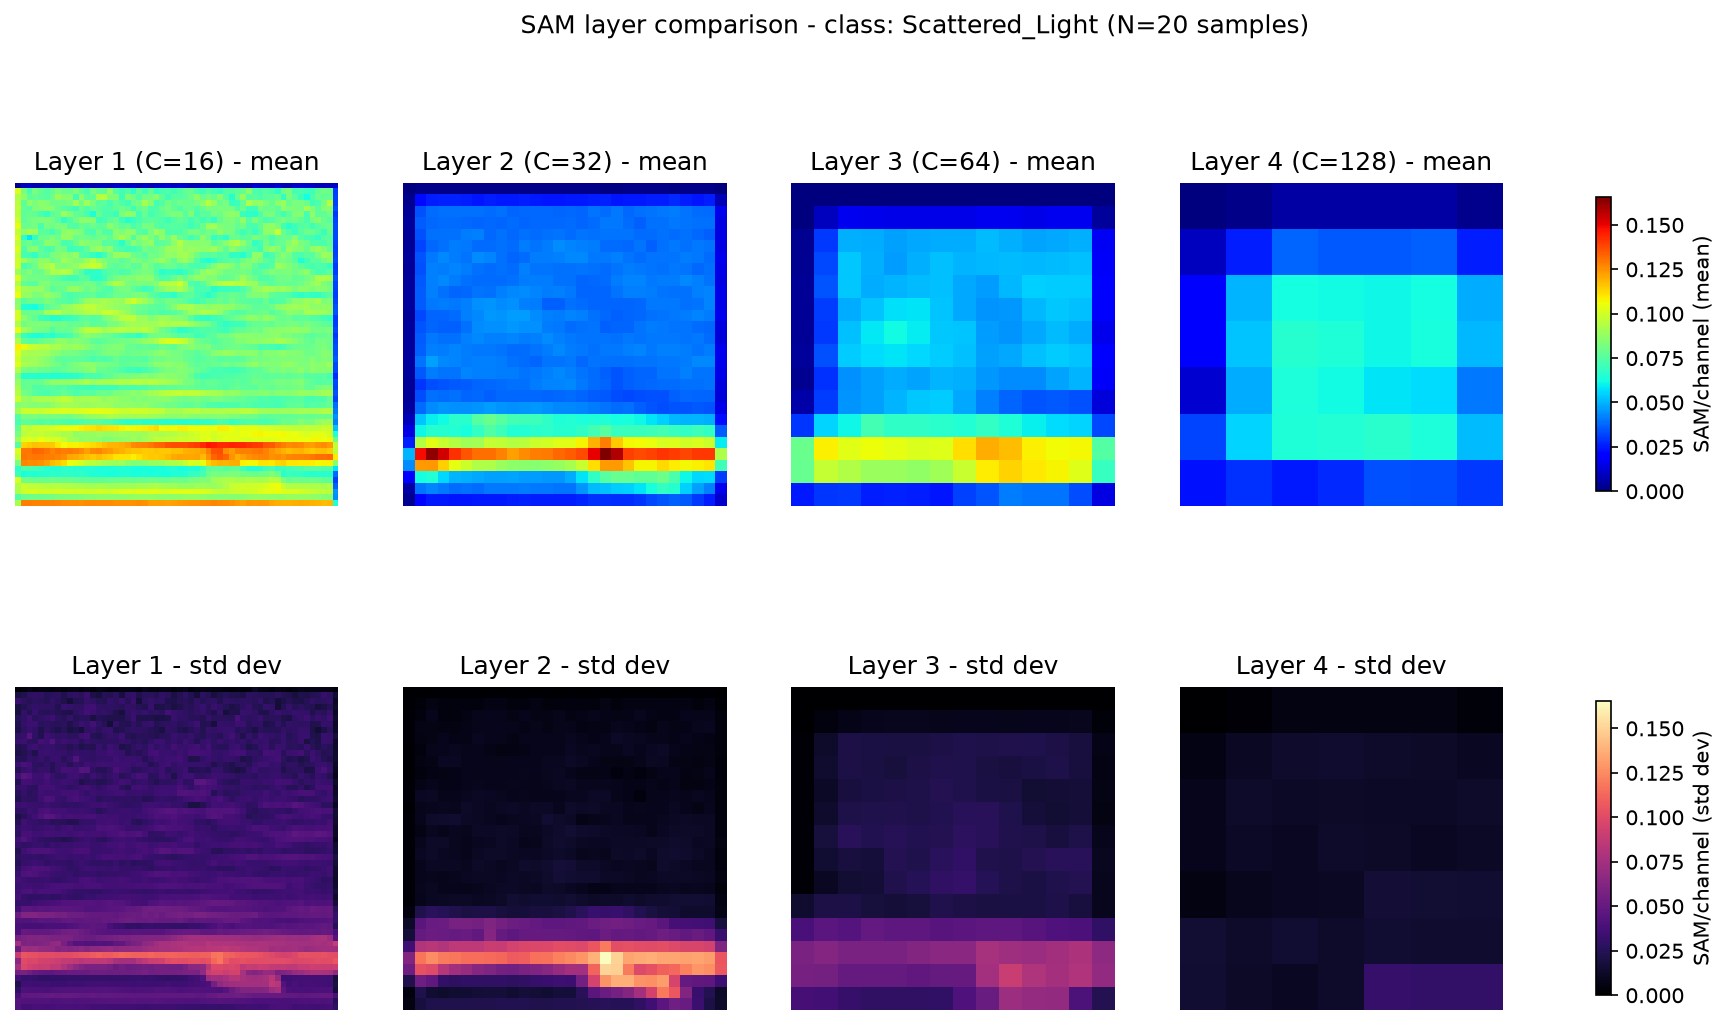
\includegraphics[width=\linewidth]{sam_layer_Scattered_Light.png}
  \caption{Scattered\_Light}
\end{subfigure}\hfill
\begin{subfigure}{0.49\linewidth}
  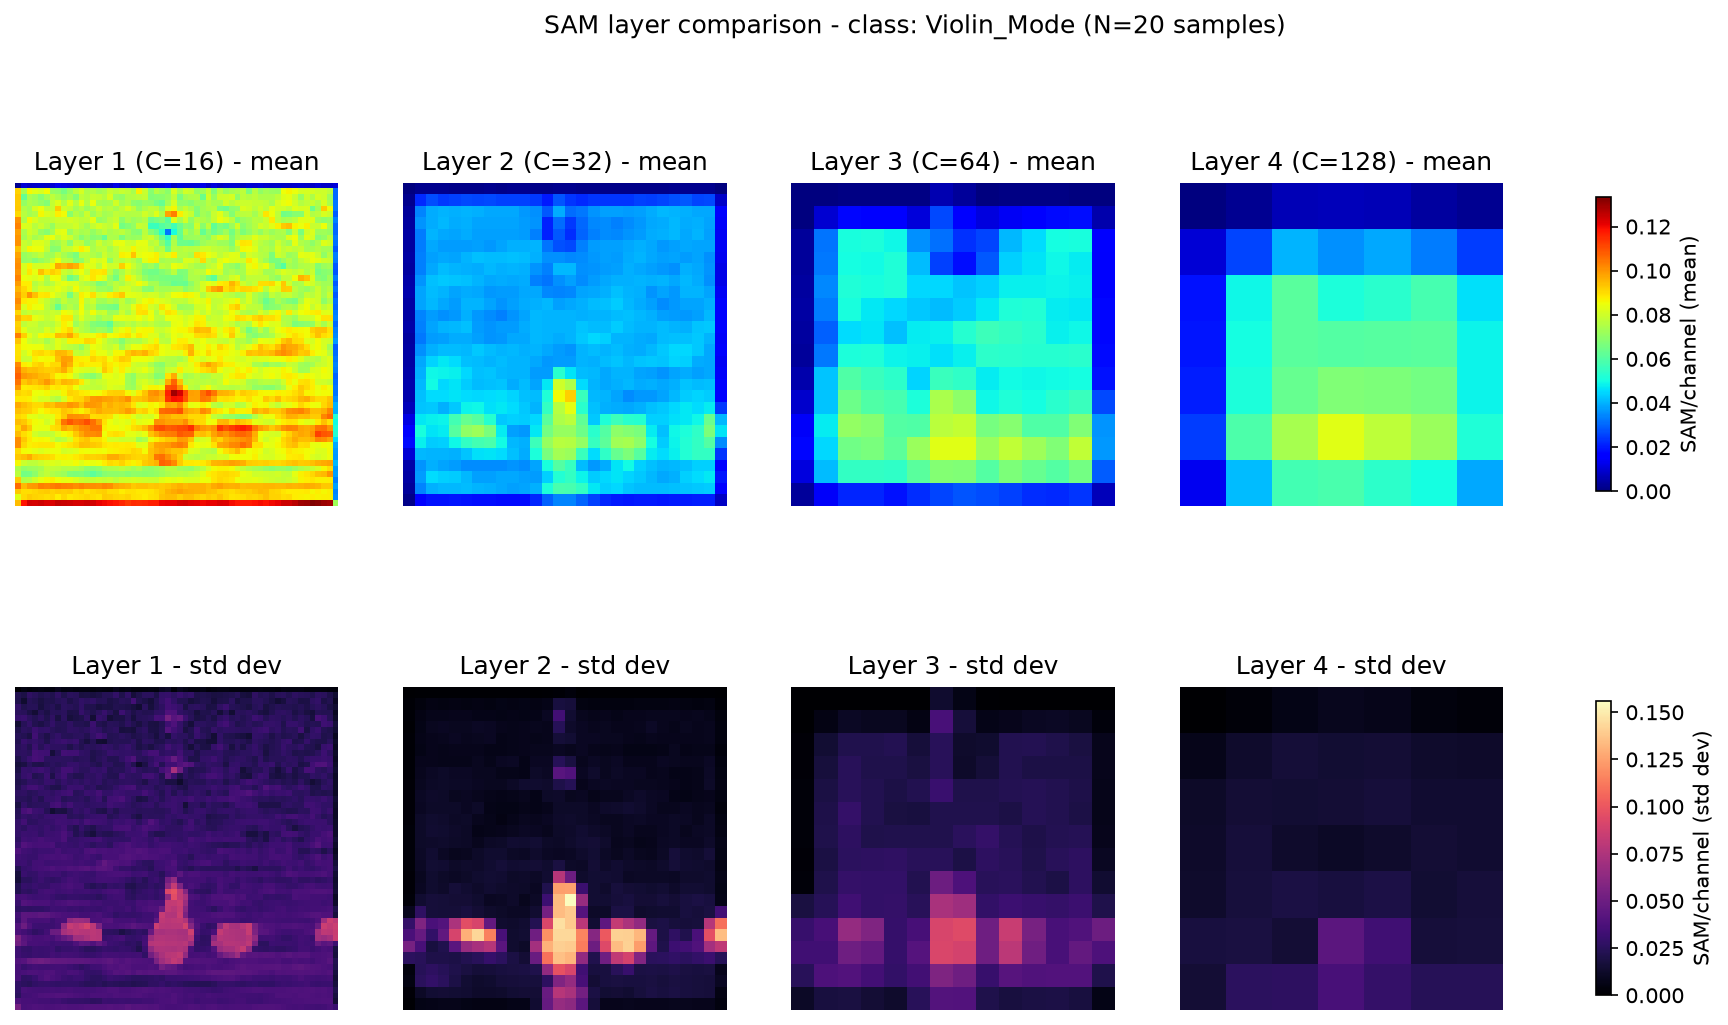
\includegraphics[width=\linewidth]{sam_layer_Violin_Mode.png}
  \caption{Violin\_Mode}
\end{subfigure}
\caption{SAM mean and standard deviation across the four hidden layers, 20
images per class, normalized by the channel count of each layer.}
\label{fig:sam-layers}
\end{figure}

\section{Fixing the explainer}

\subsection{Choice of the decay rate}
\label{sec:gamma}

SAM has one free parameter, and an explanation that changed qualitatively with an
arbitrary choice of $\gamma$ would not be trustworthy.

\textbf{$\gamma$ is the decay of a temporal kernel, so it must be evaluated on
the temporal axis.} Comparing maps averaged over time removes precisely the axis
on which $\gamma$ acts, and a high spatial correlation is then close to
guaranteed regardless of $\gamma$. Three quantities are therefore measured: the
spatial Pearson correlation between time-aggregated maps, retained for continuity
with the literature; the \emph{temporal centre of mass} of the SAM energy; and
the \emph{per-timestep correlation} against a reference $\gamma$.

Before a null result could be trusted, the instrument was checked analytically:
on a fully firing spike train with $T = 8$ the centre of mass moves from $4.86$
at $\gamma = 0.1$ to $4.02$ at $\gamma = 3.0$, so the metric does respond. A
second check comes free from the definition: at $t = 1$ the score is
$e^{-\gamma} S_0$, so changing $\gamma$ multiplies the map by a constant, and
Pearson correlation is affine-invariant. The measured per-timestep correlation at
$t = 1$ is exactly $1.000$ for every $\gamma$, as it must be.

\begin{table}[htbp]
\centering
\begin{tabular}{lcccc}
\toprule
Class & Spatial PCC, $\gamma$ 0.1 vs 3.0 & CoM at 0.1 & at 3.0 & Shift \\
\midrule
Extremely\_Loud & 0.9993 & 4.973 & 4.144 & 0.829 \\
Blip & 0.9890 & 5.192 & 4.339 & 0.853 \\
Scattered\_Light & 0.9758 & 5.271 & 4.352 & 0.919 \\
Violin\_Mode & 0.9598 & 5.260 & 4.327 & 0.933 \\
\bottomrule
\end{tabular}
\caption{$\gamma$ sensitivity at layer 2, mean over fifteen validation images per
class.}
\label{tab:gamma}
\end{table}

Two conclusions follow, and neither is the one the naive analysis would reach.

\textbf{The temporal shift is largely kernel arithmetic rather than explanation
structure.} The measured shift of $0.83$--$0.93$ steps matches what a
\emph{fully firing} spike train produces ($0.84$), whereas the layer-2 firing
rate is approximately $0.19$ and simulated random trains at that density shift by
only $0.26$ steps. SAM is therefore dominated by a minority of near-continuously
firing neurons, for which the centre of mass follows the exponential kernel. The
centre of mass against $\gamma$ is consequently \emph{not} a useful criterion for
selecting $\gamma$ --- though it remains valid as a divergence metric, where
models are compared at fixed $\gamma$ and the trivial component cancels, and it
now carries a reference scale.

\textbf{Sensitivity is strongly class-dependent.} In terms of $1 - \mathrm{PCC}$,
Violin\_Mode is 57 times more sensitive than Extremely\_Loud. The ordering
Violin\_Mode $>$ Scattered\_Light $>$ Blip $>$ Extremely\_Loud recurs identically
under the two unrelated interventions of Section~\ref{sec:calibration}.

Within $\gamma \in [0.3, 0.9]$ all per-timestep correlations remain above $0.98$
even in the worst class; only $\gamma = 3.0$ diverges appreciably.
\textbf{$\gamma = 0.5$ is adopted}, the value of the original
formulation~\cite{kim2021sam}, now supported by evidence on the axis $\gamma$
actually governs (Figure~\ref{fig:gamma}).

\begin{figure}[htbp]
\centering
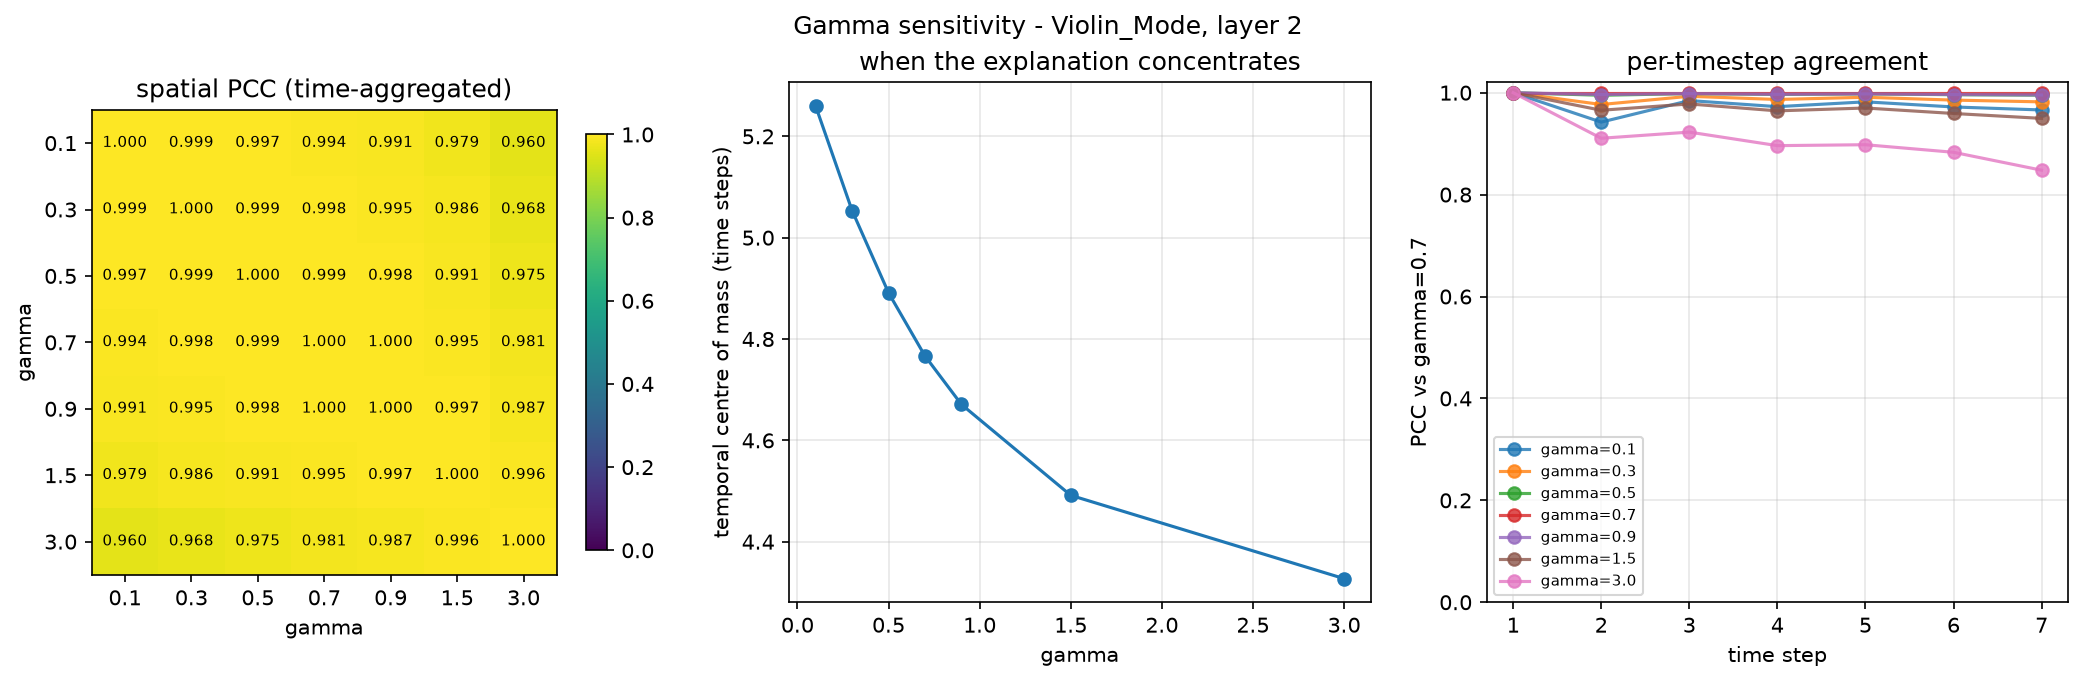
\includegraphics[width=\linewidth]{gamma_Violin_Mode.png}
\caption{$\gamma$ sensitivity for Violin\_Mode, the most sensitive class, at
layer 2. The equivalent figures for the other three classes are in
Appendix~\ref{app:figures}.}
\label{fig:gamma}
\end{figure}

\subsection{Faithfulness}
\label{sec:faithfulness}

Robustness to $\gamma$ is necessary but not sufficient: a stable explanation can
be stably wrong. The deletion metric~\cite{petsiuk2018rise} removes pixels in
decreasing order of SAM score and records the confidence assigned to the class
predicted on the unmodified image, comparing against removal in random order.

Three implementation details govern interpretation. Deleted pixels are set to
zero \emph{in normalized space}, corresponding to the dataset mean rather than to
black, a neutral substrate that avoids injecting an artificial edge. The same map
is used for both orderings. And the ordering is computed once per image and
sliced progressively, so the masked sets are nested: what is removed at 50\,\%
stays removed at 55\,\%. Regenerating a random permutation at each fraction would
break nesting for the baseline while leaving it intact for SAM, making the two
curves incomparable.

\begin{table}[htbp]
\centering
\begin{tabular}{lccccl}
\toprule
Class & AUC-SAM & AUC-random & $\Delta$ & Relative & Reading \\
\midrule
Blip & 0.3119 & 0.4795 & $-0.1676$ & $-35.0$\,\% & faithful \\
Extremely\_Loud & 0.6121 & 0.8892 & $-0.2771$ & $-31.2$\,\% & faithful \\
Scattered\_Light & 0.3835 & 0.3650 & $+0.0185$ & $+5.1$\,\% & not separable \\
Violin\_Mode & 0.4528 & 0.4540 & $-0.0012$ & $-0.3$\,\% & indistinguishable \\
\bottomrule
\end{tabular}
\caption{Deletion metric by class, 15 validation images each. A faithful
explanation gives AUC-SAM below AUC-random, so a negative $\Delta$ is expected.}
\label{tab:deletion}
\end{table}

\begin{figure}[htbp]
\centering
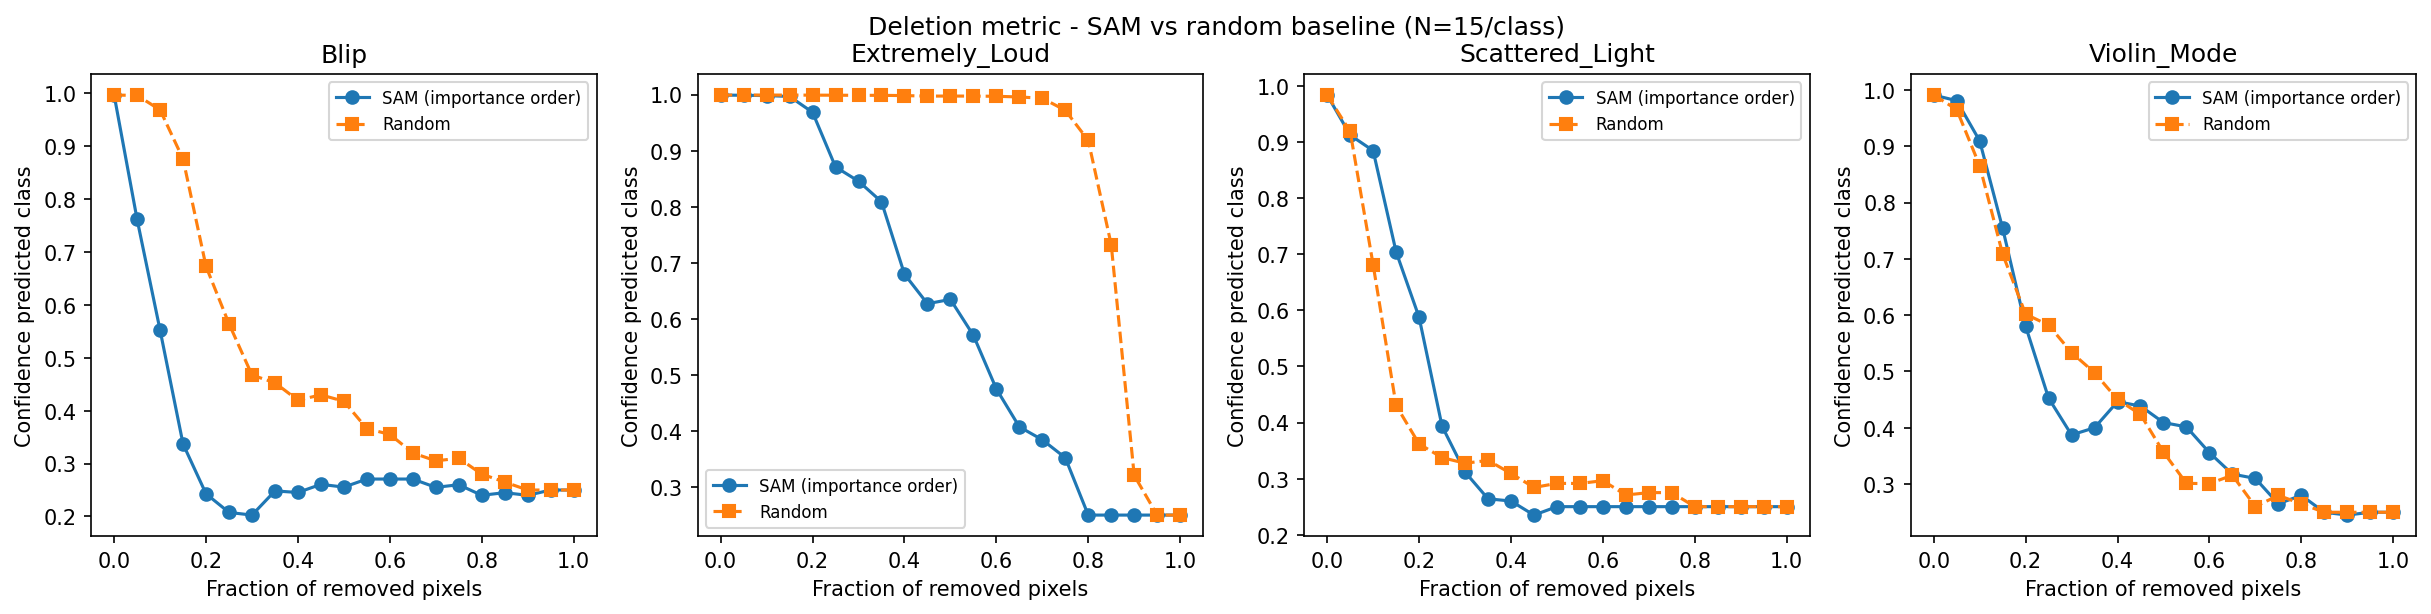
\includegraphics[width=\linewidth]{deletion_metric.png}
\caption{Deletion curves, SAM order against random order, 15 validation images
per class.}
\label{fig:deletion}
\end{figure}

The metric separates SAM from the baseline on two classes and not on the other
two, and the split is systematic. Blip and Extremely\_Loud show reductions of
$35$ and $31$\,\% in area. Violin\_Mode is within $0.3$\,\% of the baseline.
Scattered\_Light is nominally inverted, but at $+5.1$\,\% the magnitude is one
sixth of the two positive effects, so it is better described as an absence of
separation with a slight drift in the wrong direction than as a genuine reversal.

The pattern follows the spatial geometry of the classes rather than any property
of SAM. Blip is a compact vertical line and Extremely\_Loud a dominant saturated
structure, so removing the high-scoring region removes the defining evidence.
Scattered\_Light is an extended horizontal band and Violin\_Mode a set of thin
distributed lines: random deletion fragments the pattern across the whole image,
whereas SAM-guided deletion concentrates removal in one region and leaves the
rest --- which still carries sufficient evidence --- intact. This is a known
limitation of deletion-based tests, which penalize explanations of spatially
extended features, and it is reported rather than suppressed.

Two controls confirm the measurement itself. All curves converge to
approximately $0.25$ at full deletion, which is chance for four classes. And the
Extremely\_Loud random baseline remaining at $0.8892$, the highest of the four,
is independent confirmation of that class's behaviour below: its evidence is
distributed across the whole image, which is why no localized removal registers.

\section{Calibrating the divergence metrics}
\label{sec:calibration}

The metrics used to compare two explanations return numbers between zero and one
whatever is fed to them. Three questions must be answered before any quantization
result can be interpreted: what they report when nothing has changed, when
something negligible has changed, and when everything has changed.

All measurements use fifteen validation images per class at layer 2 with
$\gamma = 0.5$, on the three checkpoints of Table~\ref{tab:fp32}.

\subsection{Verification of the instrument}

Comparing a checkpoint against itself returns $\mathrm{PCC} = 1$,
$\mathrm{IoU} = 1$ and a centre-of-mass difference of $0$ to within $10^{-9}$,
confirming that the metrics and the image pairing are correct. Two separate calls
to the sampling routine return bit-identical image tensors, confirming that every
model sees the same data. A second forward pass of the same model reproduces the
maps exactly, confirming that the network is deterministic in evaluation mode and
that the cross-model differences below are not run-to-run noise.

\subsection{Two independent solutions}

\begin{table}[htbp]
\centering
\begin{tabular}{lccccc}
\toprule
Class & PCC mean & worst & IoU mean & worst & CoM diff, max \\
\midrule
Extremely\_Loud & 0.917 & 0.869 & 0.520 & 0.460 & 0.076 \\
Violin\_Mode & 0.844 & 0.816 & 0.597 & 0.543 & 0.115 \\
Blip & 0.612 & 0.336 & 0.593 & 0.503 & 0.083 \\
Scattered\_Light & 0.477 & \textbf{0.153} & 0.376 & 0.234 & 0.104 \\
\bottomrule
\end{tabular}
\caption{Divergence between full-precision models differing only in seed, over
the three seed pairs. Chance-level IoU at $k = 0.20$ is $0.111$.}
\label{tab:seeds}
\end{table}

\textbf{The spatial metrics collapse.} Two models agreeing to within one
validation sample in accuracy produce maps correlating at $0.153$ on
Scattered\_Light, with a top-20\,\% overlap of $0.234$ against a chance level of
$0.111$. For comparison, a thirtyfold change in $\gamma$ reduces the correlation
only to $0.960$: initialization variance is 21 times larger than that effect.

The per-image distribution rules out an outlier explanation. On Blip the fifteen
per-image correlations run from $0.147$ to $0.768$ with a median of $0.282$, and
twelve of the fifteen fall below $0.35$. The disagreement is uniform across
samples.

The mechanism is not a defect of the metric. Networks trained from different
initializations learn functionally equivalent but \textbf{permuted}
representations, so a pixel-wise comparison between them compares arbitrary
assignments of channels to positions rather than information content. This is why
the result is a bound on cross-model spatial claims rather than the threshold for
the quantization grid, where the quantized model inherits its parent's weights
and no permutation exists.

\textbf{The temporal centre of mass survives.} The maximum difference across seed
pairs is $0.115$ time steps, against the $\approx 0.90$ produced by a thirtyfold
change in $\gamma$ --- a factor of eight. Being an aggregate over the whole map,
it is insensitive to which neuron occupies which position, which is precisely
what defeats the pixel-wise metrics.

\subsection{A negligible perturbation}
\label{sec:perturbation}

The grid compares a quantized model with its own parent, so the operative
threshold is what a perturbation far smaller than quantization already produces.
Gaussian noise was added to the weight tensors of one checkpoint --- biases and
LIF buffers excluded, since perturbing $\beta$ would confound membrane dynamics
with weight quantization --- at magnitudes expressed as fractions of the measured
8-bit step of those weights ($0.00168$, from a maximum absolute weight of
$0.214$).

This is a graded form of the model randomization test of Adebayo et
al.~\cite{adebayo2018sanity}: where they randomize weights to verify that a
metric responds at all, this perturbs towards zero to find where it stops
responding.

\begin{table}[htbp]
\centering
\begin{tabular}{lcccc}
\toprule
Noise / 8-bit step & Extremely\_Loud & Blip & Scattered\_Light & Violin\_Mode \\
\midrule
0.01 & 1.0000 & 0.9997 & 0.9996 & 0.9991 \\
0.1  & 0.9999 & 0.9981 & 0.9977 & 0.9930 \\
0.5  & 0.9998 & 0.9949 & 0.9938 & 0.9824 \\
1.0  & 0.9997 & 0.9921 & 0.9901 & 0.9749 \\
\bottomrule
\end{tabular}
\caption{Spatial PCC against the unperturbed model. The 4-bit and 2-bit
quantization steps are 17 and 85 times larger than the largest perturbation
shown.}
\label{tab:perturbation}
\end{table}

\textbf{The spatial metrics are usable after all, for same-parent comparisons.}
PCC remains above $0.975$ under a perturbation as large as the entire 8-bit step.
The collapse of Table~\ref{tab:seeds} is a consequence of comparing different
initializations, not a fragility of the metric; the two results answer different
questions.

\textbf{The metrics differ sharply in dynamic range.} Measuring the distance from
perfect agreement, PCC starts $0.025$ away from $1$ and can reach $0.847$: 34
times its own floor. IoU starts $0.296$ away and reaches $0.766$, a factor of
only $2.6$, and is already at $0.704$ under a perturbation 85 times smaller than
the 2-bit step. IoU should therefore be read as a sensitive early indicator that
a change has occurred, and PCC as the graded measure of how large it is. The
temporal centre of mass sits between them, with a factor of $3.9$ between its
numerical floor ($0.029$ steps) and the seed level ($0.115$).

\textbf{Extremely\_Loud does not respond.} Its PCC is $0.9997$ under the largest
perturbation and its worst per-timestep correlation is $0.996$. Combined with its
behaviour under $\gamma$, this class cannot register an explanation change by any
measure tested here. A flat grid result for Extremely\_Loud will not distinguish
absence of effect from inability to detect one, and this is stated in advance.

\subsection{What the calibration establishes}

\begin{table}[htbp]
\centering
\begin{tabular}{llccc}
\toprule
Level & What it measures & PCC & IoU & CoM \\
\midrule
Numerical floor & Weight noise at $1\times$ the 8-bit step & 0.975 & 0.704 & 0.029 \\
$\gamma$ reference & A thirtyfold change in the kernel & 0.960 & --- & 0.90 \\
Independent solutions & Two FP32 models, different seeds & 0.153 & 0.234 & 0.115 \\
\bottomrule
\end{tabular}
\caption{The three calibration levels, worst class in each case, at 112\,px,
layer 2, $\gamma = 0.5$, on validation.}
\label{tab:calibration}
\end{table}

The \emph{numerical floor} is the operative threshold for the grid: a divergence
below what a negligible weight perturbation already produces is measurement
noise. The \emph{$\gamma$ reference} gives an intuition: if quantization produced
a PCC of $0.90$, it would be doing more than a thirtyfold change of the explainer
itself. The \emph{independent-solutions} level is a pessimistic upper bound and a
result in its own right.

The class sensitivity ordering --- Violin\_Mode $>$ Scattered\_Light $>$ Blip $>$
Extremely\_Loud --- recurs identically under three unrelated interventions:
changing the kernel, changing the initialization, and perturbing the weights.
Explanation sensitivity is therefore a property of the class morphology, and
every grid result must be reported per class, since a pooled figure would average
a class that responds strongly with one that does not respond at all.


\section{Preparing the membrane arm}
\label{sec:membrane-prep}

\subsection{The range of the membrane potential}

The membrane potential of every LIF layer was recorded at every time step over
the full validation partition ($1\,435$ images, eight steps) on the reference
checkpoint. Table~\ref{tab:membrane-range} summarizes the distributions.

\begin{table}[htbp]
\centering
\begin{tabular}{lccccccc}
\toprule
Layer & min & $p_{0.1}$ & median & $p_{99.9}$ & max & std & $> U_{\text{thr}}$ \\
\midrule
1 & $-12.75$ & $-9.43$  & $-0.08$ & 6.40  & 8.76  & 1.98 & 14.9\,\% \\
2 & $-15.73$ & $-11.10$ & $0.25$  & 5.63  & 11.64 & 1.42 & 15.1\,\% \\
3 & $-47.03$ & $-36.82$ & $0.00$  & 11.27 & 20.23 & 4.22 & 15.3\,\% \\
4 & $-26.04$ & $-17.01$ & $-0.62$ & 6.34  & 14.67 & 2.59 & 11.5\,\% \\
\bottomrule
\end{tabular}
\caption{Membrane potential of the four hidden layers over the validation
partition, reference checkpoint (seed 1234). The last column is the fraction of
values above the firing threshold $U_{\text{thr}} = 1$, which equals the mean
firing rate of the layer.}
\label{tab:membrane-range}
\end{table}

The distributions are wide and strongly skewed towards negative values: in
layer 3 the potential reaches $-47$, almost fifty thresholds below rest. A grid
covering the full observed range would be dominated by values far from the
threshold, which is the only point at which a potential affects a spike
decision. At 4 bits, a symmetric grid over $[-47, +47]$ would have a step of
more than six thresholds, and the network could not be represented at all.

\subsection{Clipping the potential costs nothing}

Before any quantization, the potential of the four hidden layers was
\emph{clipped} at every time step to a candidate range, on the full-precision
network, and the effect on accuracy and dynamics was measured. Clipping isolates
the choice of range from the choice of bit-width: if a range already changes the
network in full precision, no grid built on it can be faithful.

\begin{table}[htbp]
\centering
\begin{tabular}{lccc}
\toprule
Clipping range & Val.\ accuracy & $\Delta$ samples & Layer-4 CoM \\
\midrule
none                         & 0.98328 & ---  & 3.9469 \\
per layer, $[p_{0.1}, p_{99.9}]$ & 0.98328 & 0 & 3.9469 \\
per layer, $[p_{1}, p_{99}]$     & 0.98328 & 0 & 3.9469 \\
fixed $[-8, +4]$             & 0.98328 & 0    & 3.9469 \\
fixed $[-4, +4]$             & 0.98328 & 0    & 3.9469 \\
fixed $[-2, +2]$             & 0.98258 & $-1$ & 3.9415 \\
unsigned $[0, +4]$           & 0.98258 & $-1$ & 3.9483 \\
\textbf{unsigned $[0, +2]$}  & \textbf{0.98258} & $\mathbf{-1}$ & \textbf{3.9431} \\
control $[-0.5, +0.5]$       & 0.84808 & $-194$ & 4.0684 \\
\bottomrule
\end{tabular}
\caption{Effect of clipping the hidden membrane potentials on the
full-precision reference (seed 1234), on validation. The tolerance is the spread
of the three-seed reference, four samples out of $1\,435$. The last column is the
temporal centre of mass of the layer-4 spike counts.}
\label{tab:clipping}
\end{table}

Three observations follow from Table~\ref{tab:clipping}.

\textbf{Negative potentials carry no information the network uses.} Clipping to
$[0, 2]$ removes every negative value --- in layer 3 a range of 47 thresholds ---
and costs one validation sample out of $1\,435$, a quarter of the spread between
seeds. The per-layer dead fractions are unchanged to the first decimal
(16.1 / 12.5 / 11.3 / 22.5\,\% against 16.1 / 12.6 / 11.3 / 22.8\,\%), and the
largest shift in the temporal centre of mass of any layer's spike counts is
$0.004$ steps, well below the $0.029$-step floor measured for the SAM centre of
mass in Section~\ref{sec:calibration} (the two quantities are related but not
identical). Below rest, how far below no longer matters: a
neuron at $-20$ and a neuron at $0$ both need more than one threshold of input
to fire.

\textbf{The upper bound can be tight.} Potentials above twice the threshold are
rare and can be clipped at no measurable cost. Since the clipping acts after the
spike decision, it only alters the carried state of neurons that have just fired
well above threshold; the spike they emitted at that step is unaffected.

\textbf{The clipping is not inert.} The control range $[-0.5, +0.5]$, which
keeps the potential permanently below threshold after each step, drops accuracy
to $0.848$ and raises the layer-3 firing rate from $0.153$ to $0.227$. The hook
therefore acts on the state the network actually carries, and the null results
above are genuine.

The unsigned range $[0, 2]$ is adopted: it is the tightest range tested that
stays within tolerance, it centres the threshold in the grid, and it spends no
levels on negative values, which saves one bit at every bit-width compared with
the symmetric $[-2, 2]$ that performs identically.

\section{Energy and memory of the reference}
\label{sec:energy-fp32}

Table~\ref{tab:energy-fp32} applies the accounting of
Section~\ref{sec:energy-method} to the full-precision reference, using the
per-hidden-layer firing rates averaged over the three seeds
($0.258 / 0.186 / 0.185 / 0.126$).

\begin{table}[htbp]
\centering
\begin{tabular}{lrrr}
\toprule
Layer & MAC (dense) & Operations & Energy ($\mu$J) \\
\midrule
conv1 (analog input, once) & $3.76 \times 10^{6}$ & $3.76 \times 10^{6}$ MAC & 17.31 \\
conv2 & $10.04 \times 10^{6}$ & $20.72 \times 10^{6}$ SOP & 18.65 \\
conv3 & $10.04 \times 10^{6}$ & $14.93 \times 10^{6}$ SOP & 13.44 \\
conv4 & $10.04 \times 10^{6}$ & $14.83 \times 10^{6}$ SOP & 13.34 \\
linear & $0.03 \times 10^{6}$ & $0.03 \times 10^{6}$ SOP & 0.02 \\
\midrule
\textbf{SNN, conv1 once} & & & \textbf{62.8} \\
SNN, conv1 at every step & & & 183.9 \\
Equivalent CNN (all MAC) & $33.89 \times 10^{6}$ & & 155.9 \\
\bottomrule
\end{tabular}
\caption{Estimated energy per inference of the FP32 reference at 112\,px,
$T = 8$, with 45\,nm costs of 4.6\,pJ per MAC and 0.9\,pJ per accumulate.}
\label{tab:energy-fp32}
\end{table}

The spiking network costs $62.8\,\mu$J per inference, $2.5$ times less than a
convolutional network of identical shape. The saving depends entirely on the
treatment of the first layer: recomputing its constant current at every step
would cost $183.9\,\mu$J, more than the convolutional equivalent, and the two
readings differ by a factor of $2.9$. Even computed once, the first convolution
is $28\,\%$ of the budget, because it is the only layer that multiplies.

The initialization regime of Section~\ref{sec:hyperparameters} reaches the
energy as well. Computed seed by seed, the estimate is $50.0$, $78.1$ and
$60.1\,\mu$J for seeds 1234, 2345 and 3456, the difference coming almost
entirely from the first two layers, where the firing regime varies most. Three
models indistinguishable in accuracy therefore differ by more than half in
estimated energy, and every energy comparison in the grid is made at matched
seed.

In memory, the 295\,332 weights occupy $1\,154$\,KiB in 32-bit float, and the
membrane state of the $94\,080$ hidden neurons another $368$\,KiB. At 8, 4 and 2
bits these become $288$, $144$ and $72$\,KiB for the weights and $92$, $46$ and
$23$\,KiB for the state.

\section{The quantization grid}
\label{sec:grid-results}

\todo{Everything in this section depends on the grid (schedule: launch 4
October, GATE 2 on 7 October). The structure, tables and the questions each
subsection must answer are in place; fill them from
\texttt{results/grid/}, \texttt{results/divergence.json},
\texttt{results/cross\_faithfulness.json}, \texttt{results/stratified.json} and
\texttt{results/energy.json}. Report every table per class and with the
three-seed spread.}

\subsection{Sanity gate}

The joint 8-bit model of seed \tbd{} reaches \tbd{} validation accuracy against
\tbd{} for its parent, a difference of \tbd{} samples out of $1\,435$, within
the four-sample tolerance. \todo{Report the number even if the gate passes
trivially: it is the check that separates a bug from a result.}

\subsection{Accuracy}

\begin{table}[htbp]
\centering
\begin{tabular}{lcccc}
\toprule
Arm & 32 bit & 8 bit & 4 bit & 2 bit \\
\midrule
Weight-only   & 0.9833 & \tbd & \tbd & \tbd \\
Membrane-only & 0.9833 & \tbd & \tbd & \tbd \\
Joint         & 0.9833 & \tbd & \tbd & \tbd \\
\bottomrule
\end{tabular}
\caption{Validation accuracy across the grid, mean over three seeds.}
\label{tab:grid-accuracy}
\end{table}

\todo{Add per-class recall (as Table~\ref{tab:fp32}) and the relative $L_2$
distance of the quantized weights from the parent, per layer. Comment on whether
2-bit membrane collapses as predicted by Table~\ref{tab:membrane-grid}.}

\subsection{Explanation divergence}

\begin{table}[htbp]
\centering
\small
\begin{tabular}{llcccc}
\toprule
Arm, bits & Metric & Blip & Extremely\_Loud & Scattered\_Light & Violin\_Mode \\
\midrule
W, 8 & PCC / CoM & \tbd & \tbd & \tbd & \tbd \\
W, 4 & PCC / CoM & \tbd & \tbd & \tbd & \tbd \\
W, 2 & PCC / CoM & \tbd & \tbd & \tbd & \tbd \\
U, 8 & PCC / CoM & \tbd & \tbd & \tbd & \tbd \\
U, 4 & PCC / CoM & \tbd & \tbd & \tbd & \tbd \\
U, 2 & PCC / CoM & \tbd & \tbd & \tbd & \tbd \\
W+U, 8 & PCC / CoM & \tbd & \tbd & \tbd & \tbd \\
W+U, 4 & PCC / CoM & \tbd & \tbd & \tbd & \tbd \\
W+U, 2 & PCC / CoM & \tbd & \tbd & \tbd & \tbd \\
\midrule
\multicolumn{2}{l}{Numerical floor (Table~\ref{tab:calibration})} & 0.9921 / --- & 0.9997 / --- & 0.9901 / --- & 0.9749 / --- \\
\bottomrule
\end{tabular}
\caption{Spatial PCC and temporal CoM difference against the parent at the same
seed, layer 2, $\gamma = 0.5$, fifteen validation images per class, mean over
three seeds. Values beyond the numerical floor are a measured effect.}
\label{tab:grid-divergence}
\end{table}

\todo{Fill from \texttt{divergence.json}; add the per-class CoM floors from the
perturbation experiment in the last row (only the worst-class value, $0.029$, is
currently in the text), and give IoU and SSIM in an analogous table. Plot the
per-timestep correlation curves for U-only against W-only at 4 bits.}

\subsection{The hypothesis}

\todo{The single paragraph the thesis is built around. State at which bit-width
the U-only arm first displaces the CoM beyond $0.029$ steps and at which
bit-width the W-only arm first lowers PCC below the floor, per class; conclude
whether the ordering predicted in Chapter~\ref{ch:introduction} holds. If the
CoM never moves, check first that the temporal metric is not insensitive in
this regime (Section~\ref{sec:gamma}: the CoM is dominated by near-continuously
firing neurons).}

\subsection{Faithfulness and behaviour}

\todo{Cross-faithfulness on Blip and Extremely\_Loud (own map vs parent map);
EMD between firing-rate distributions, compared with the range reported by
Smith et al.\ and with the seed-to-seed value of $0.039$; dead and saturated
fractions and CV-ISI per configuration.}

\subsection{Stratification by event strength}

\todo{Divergence per within-class SNR tercile, for each arm. Prediction:
steep dependence for the membrane arm, flatter for weights. Characterize the
disagreement subset by its physical descriptors.}

\subsection{Accuracy, fidelity and energy}

\todo{Energy and memory per configuration (extend Table~\ref{tab:energy-fp32}
with the integer coefficients and the per-layer rates measured on each quantized
checkpoint), then the concluding figure: accuracy, explanation fidelity and
energy on a common bit-width axis. Identify, if it exists, the operating point
where accuracy is intact and energy reduced but the explanation has diverged.}

\section{Test-set evaluation}
\label{sec:test}

\begin{table}[htbp]
\centering
\begin{tabular}{lcc}
\toprule
Model & Test accuracy & 95\,\% Wilson interval \\
\midrule
FP32 reference & \tbd & \tbd \\
\tbd{} (selected quantized) & \tbd & \tbd \\
\bottomrule
\end{tabular}
\caption{Accuracy on the test partition ($1\,436$ images), opened once.}
\label{tab:test}
\end{table}

\todo{Run \texttt{evaluate\_test.py} once, after every design decision
(schedule: 11 October). Add per-class recall.}

\chapter{Discussion and Conclusions}
\label{ch:conclusions}

\section{The instrument}

This thesis set out to measure whether a quantized spiking neural network
reasons like its full-precision parent, and found that the measurement could not
be interpreted until the instrument was calibrated.

A four-block convolutional spiking network classifies four families of transient
noise in LIGO data at $0.9833 \pm 0.0014$ validation accuracy over three seeds,
under constraints --- shift-implementable membrane decay, at most eight time
steps, 112-pixel input --- that keep the configuration deployable by
construction rather than by subsequent rounding. Each of those constraints was
shown to cost nothing measurable in accuracy, and the resolution choice improved
the health of the deepest layer by 12.7 percentage points of dead fraction.

The Spike Activation Map was implemented, its summation range corrected, and its
free parameter fixed on the temporal axis it governs rather than on
time-aggregated maps that cannot see it. Its faithfulness was tested
quantitatively and found to hold on two classes of four, with a geometric
explanation for the other two.

The calibration established three levels: the divergence produced by weight noise
as large as an entire 8-bit quantization step (PCC $0.975$), by a thirtyfold
change in the explainer (PCC $0.960$), and by initialization alone (PCC $0.153$).
The third is far larger than expected, and it carries three consequences.

\paragraph{Spatial metrics cannot compare independently trained models.} Two
networks that agree to within one validation sample in accuracy produce
explanations correlating at $0.153$. The mechanism is representational
permutation rather than any defect of the metric, and the disagreement is uniform
across samples rather than driven by outliers.

\paragraph{They can compare a model with its own parent.} Under a perturbation 85
times smaller than the 2-bit quantization step, PCC remains above $0.975$. The
two results answer different questions, and the distinction must be made
explicitly whenever such a number is reported. In this thesis it decided the
design of the grid: every quantized model is fine-tuned from its own parent.

\paragraph{Published figures are not interpretable without these floors.} Values
around $0.85$ are presented in the literature as evidence of preserved
explanations. For this architecture that value falls between the numerical floor
and the independent-solutions level, so it cannot be read without knowing which
comparison produced it. Establishing the floors requires no training runs beyond
a multi-seed baseline that is good practice regardless.

A fourth observation cuts across all of them: the class sensitivity ordering is
identical under three unrelated interventions. Explanation sensitivity is a
property of the class morphology, not of the perturbation applied, and
Extremely\_Loud --- saturated and spatially extensive --- registers no change
under any measure tested.

The preparation of the membrane arm added a result of its own: the network makes
no use of negative membrane potentials. Clipping the hidden state to $[0, 2]$,
which removes up to 47 thresholds of negative range, costs one validation sample
and leaves the dynamics unchanged, so the membrane can be stored on an unsigned
grid at one bit less than a symmetric one would need.

\section{Quantization and explanation fidelity}

\paragraph{Accuracy is not a sufficient criterion for spiking networks either.}
The finding of Rabbi et al.~\cite{rabbi2026} on convolutional networks carries
over, in a sharper form. Two configurations of this network classify equally
well, a 4-bit weight model and a 2-bit membrane model, and their explanations
differ by a factor of almost two in agreement with the original. Anyone selecting
a configuration on accuracy alone could have chosen the second and deployed a
model that reaches the right labels while showing a different part of the
spectrogram. In the detector-characterization setting of
Chapter~\ref{ch:introduction}, that is the scenario that matters: the label is
correct, the diagnostic cue is not the one the original model would have given.

\paragraph{The divergence is real but bounded.} The changed explanations are
still faithful: deleting the pixels they highlight degrades the model's
confidence almost as much as deleting the parent's highlights does, and the
quantized model can be explained with its parent's maps as well as with its own.
The quantized network has not stopped using spectrogram evidence; among
several redundant sets of evidence it now highlights a different one. A
faithfulness test alone would have declared the explanation intact; an overlap
test alone would have suggested it was lost. Both are needed to say what
happened.

\paragraph{The hypothesis was wrong in its form and right in its mechanism.}
The prediction that the membrane would move the temporal axis of the explanation
before the weights moved its spatial axis is not supported: both arms first
register at 4 bits, and at 2 bits the membrane changes where the explanation
points more than when. What the membrane does change first is the temporal
dynamics of the network itself: at 2 bits, with a single representable level
between rest and threshold, the first layer fires with perfectly regular
intervals. The temporal centre of mass, built to capture the time axis of the
explanation, is blind to this, because it measures where the spike mass falls,
not how it is spaced. A temporal explanation metric for spiking networks needs
to see regularity as well as timing, and the present instrument does not.

\paragraph{The comparison with Smith et al.\ inverts.} Smith et
al.~\cite{smith2026} report that the membrane needs at least four bits while
learned weights survive two. The weight result agrees with theirs: uniform ternary weights fail, where they
needed a learned quantizer to keep two bits. The membrane result does not: with
a grid fitted to the measured range, a 2-bit membrane keeps accuracy at parity,
where they lose $4$--$8\,\%$.

\paragraph{Weak events are not where the explanation fails.} The expectation that
quantization would disturb spike decisions mostly in weak events, whose
potentials sit near threshold, finds no consistent support: the gradient with
event strength changes sign across seeds. The only consistent effect is
reversed: the most saturated Extremely\_Loud events lose their explanation most,
because their evidence is spread over the whole image and the highlighted region
is least constrained.

\paragraph{Efficiency and explainability do not trade off here.} The
configuration that changes the explanation at constant accuracy is the
2-bit membrane, and it is the one that saves no energy: with weights in full
precision the per-operation cost stays the same while firing rates rise. The
deployable configuration, joint 4-bit, keeps accuracy at parity and the
explanation at the numerical floor, at about one sixtieth of the estimated
energy and one eighth of the memory. The divergence between the three curves of
Figure~\ref{fig:headline} exists, but it occurs at a point no one would choose
for efficiency.

\paragraph{Seed variance is the dominant source of variation.} Three
full-precision networks of equal accuracy differ by a factor of 2.6 in the
firing rate of their first layer, by more than half in estimated energy, and in
which classes SAM can explain faithfully at all. The 2-bit membrane IoU ranges
from $0.26$ to $0.62$ across seeds. Every comparison in this thesis was made
within a seed, and a single-seed study of the same question could have reached
any conclusion from ``the explanation is preserved'' to ``it is lost''.

\section{Limitations}

\paragraph{Generalization of the thresholds.} The three calibration levels are
specific to this architecture, this dataset and this explainer. The
\emph{mechanism} behind the collapse, representational permutation between
independently trained networks, is general and well documented; the
\emph{magnitude} is not, and a different architecture could place the floors
elsewhere. What generalizes is the claim that the floors must be measured, not
the values measured here.

\paragraph{Labels are model output.} Accuracy is agreement with the Gravity Spy
convolutional classifier rather than with physical ground truth. A model that
reproduced that classifier's systematic errors would score well here. The
per-class confidences are available and would permit stratifying accuracy by the
reference classifier's own certainty, which was not done.

\paragraph{The partition is random with respect to time.} If glitches of the same
class are correlated within observing periods, a random test set overestimates
generalization to new periods. A block split by observing run would be the more
conservative validation; the timestamps were dropped during feature selection for
the reasons given in Chapter~\ref{ch:methodology} and would have to be recovered.

\paragraph{$T$ sits at the imposed ceiling.} The search was forbidden from
exploring more than eight time steps, so it is not known whether it would have
preferred a longer integration window. An unconstrained search selected seven,
which bounds the likely cost but does not eliminate the question.

\paragraph{The deletion metric fails on two classes.} The geometric explanation
offered in Section~\ref{sec:faithfulness} --- that deletion-based tests penalize
spatially extended evidence --- is an interpretation, not a demonstration. An
insertion curve, which rewards rather than penalizes distributed evidence, would
test it directly.

\paragraph{The explanation is class-agnostic.} SAM does not use labels, so the
deletion metric measures faithfulness to the model's \emph{predicted} class. This
is the correct reading of the metric and matches its original formulation, but it
means misclassified examples are informative and should be inspected separately
rather than pooled.

\paragraph{The temporal metric is partly kernel arithmetic.} The $\gamma$
analysis showed that the centre of mass of the SAM energy is dominated by a
minority of near-continuously firing neurons. Between models compared at the same
$\gamma$ this component cancels, but it means that the CoM is most sensitive to
changes in that minority and may under-report changes elsewhere.

\paragraph{Quantization is simulated.} Fake quantization reproduces the values an
integer implementation would hold, not its arithmetic: the membrane is quantized
as a stored state after each spike decision, while on integer hardware the
comparison with threshold would itself be performed on integers. The energy
figures are analytical, at a 45\,nm reference node, and below eight bits they
rest on an extrapolation of the per-operation costs.

\paragraph{Sample sizes of the explanation analyses.} Divergence is measured on
twenty validation images per class, faithfulness on ten, stratification on
fifteen per class and tercile, and the membrane range on a single checkpoint.
These are sufficient for the effects reported here, which are large, but limit
the resolution with which small differences between configurations can be
ranked; the faithfulness analysis covers only the 2-bit membrane arm.

\paragraph{One grid, one fitting procedure.} Each bit-width was fitted once per
seed, with one fine-tuning schedule and one membrane range. The collapse of the
2-bit weight arm and the survival of the 2-bit membrane are properties of these
quantizers; a different weight quantizer (learned scales, a wider grid for the
readout) could move the weight arm's breaking point.

\paragraph{The control does not isolate the fine-tuning.} Fine-tuning without a
quantizer never improved the parent's validation accuracy, so the selected
control checkpoint is the parent itself. The control therefore shows that the
pipeline is inert, but not what the extra epochs alone would do to a model that
does change; the quantized checkpoints combine both effects.

\paragraph{Checkpoints are selected on the validation partition} on which they
are then analyzed. With selection by accuracy and analysis of explanations, the
dependence is weak, but the test-set evaluation is the only fully independent
estimate.

\paragraph{The saving factor rests on an assumption.} Costing the analog first
convolution at the weight bit-width gives a joint 4-bit saving of 62; costing it
in floating point gives 3.5. The operation counts, the memory and the ranking of
configurations do not depend on it.

\section{Future work}

\paragraph{Deployment.} Hardware deployment was deliberately left out of scope.
The natural continuation is to export the selected integer configuration to a
neuromorphic platform or a microcontroller, and to measure on it the latency,
energy and memory that are estimated analytically here.

\paragraph{Normalization.} The baseline contains no batch normalization, because
quantizing its parameters is a problem distinct from quantizing weights and
potentials. Deeper spiking networks need it, and both approximating it with shifts
and removing it altogether through progressive training are available; repeating
the study on a normalized architecture would test whether the conclusions survive.

\paragraph{The temporal axis of the input.} Under direct encoding every temporal
structure is generated by the network. Feeding the spectrogram column by column,
so that time in the input corresponds to time in the signal, would give the
temporal explanation a physical meaning and make the temporal metrics measure
something a detector scientist can read.

\paragraph{Wider benchmark.} Extending the four classes to the full Gravity Spy
taxonomy, with a split by observing run, would make the classification results
comparable with the published benchmark.

\section{Closing remark}

Compressed models are increasingly deployed where their explanations are acted
upon. This thesis asked whether a quantized spiking network still decides for
the same reasons as the network it came from, and found that the question has
two prerequisites: knowing what the comparison metrics report when nothing has
changed, and comparing every model with its own parent. With both in place, the
answer for this network is that it mostly does --- down to four bits, in every
arm --- and that the one configuration that does not is invisible to accuracy,
partly invisible to correlation and to faithfulness, and visible to a metric
that asks which pixels a reader is shown. That is the configuration a
deployment chosen on accuracy could have picked, and the reason the question was
worth asking.

%-------------------------------------------------------------------------------
% \backmatter
%-------------------------------------------------------------------------------
%---------------------------------------
% References
%---------------------------------------
\clearpage
\phantomsection
\addcontentsline{toc}{chapter}{References}
\bibliographystyle{plain}
\bibliography{references}

%---------------------------------------
% Appendices
%---------------------------------------
\appendix

\chapter{Additional figures}
\label{app:figures}

\begin{figure}[htbp]
\centering
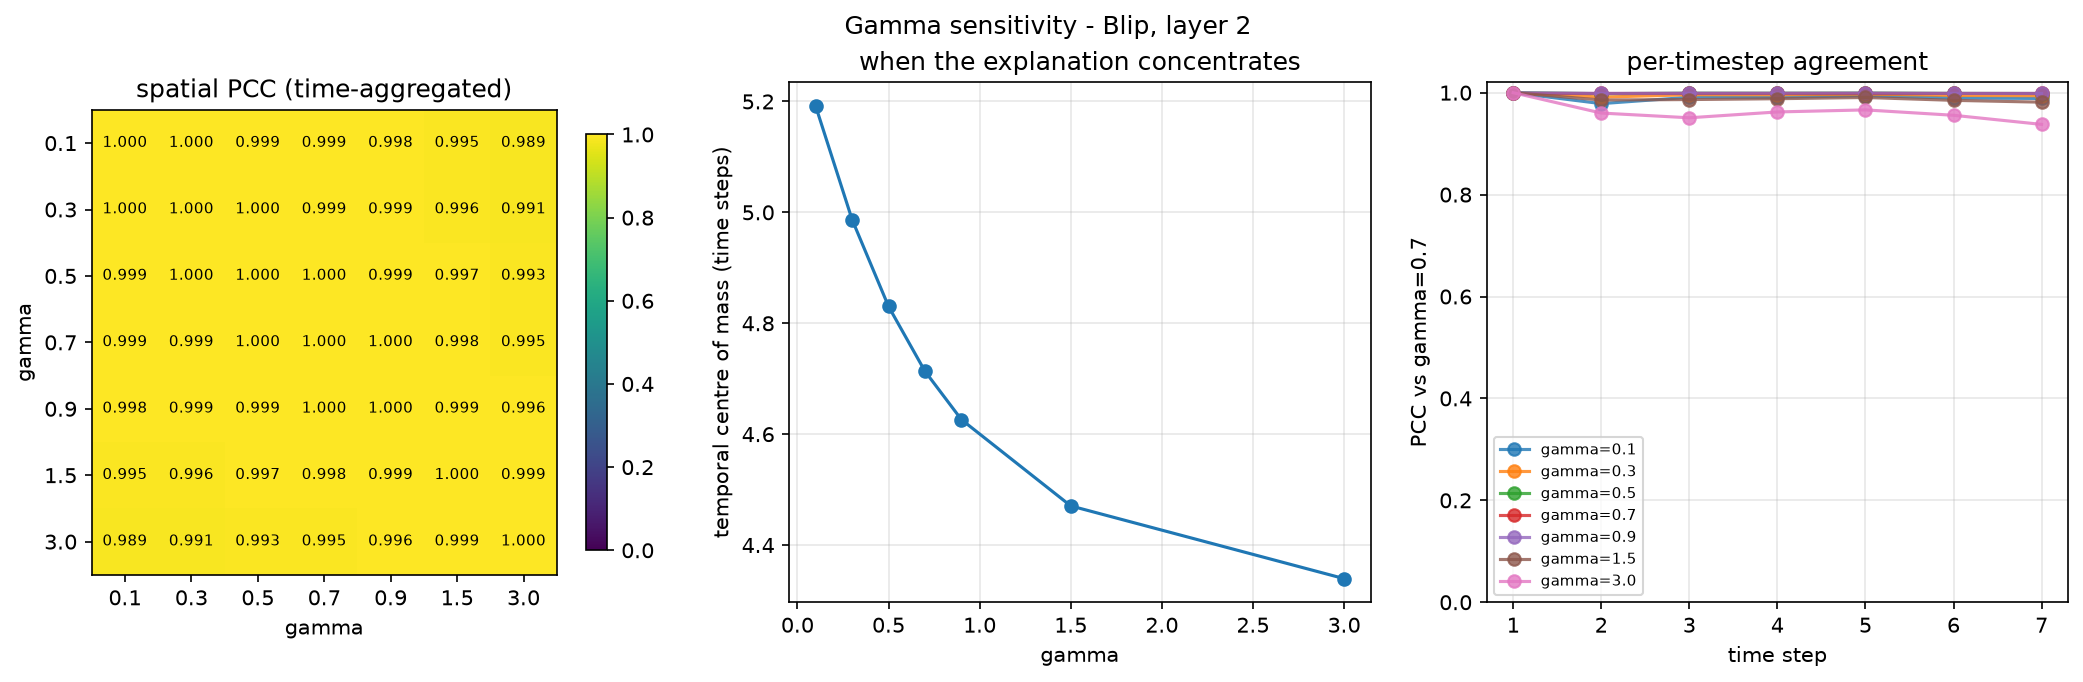
\includegraphics[width=\linewidth]{gamma_Blip.png}\\[0.5em]
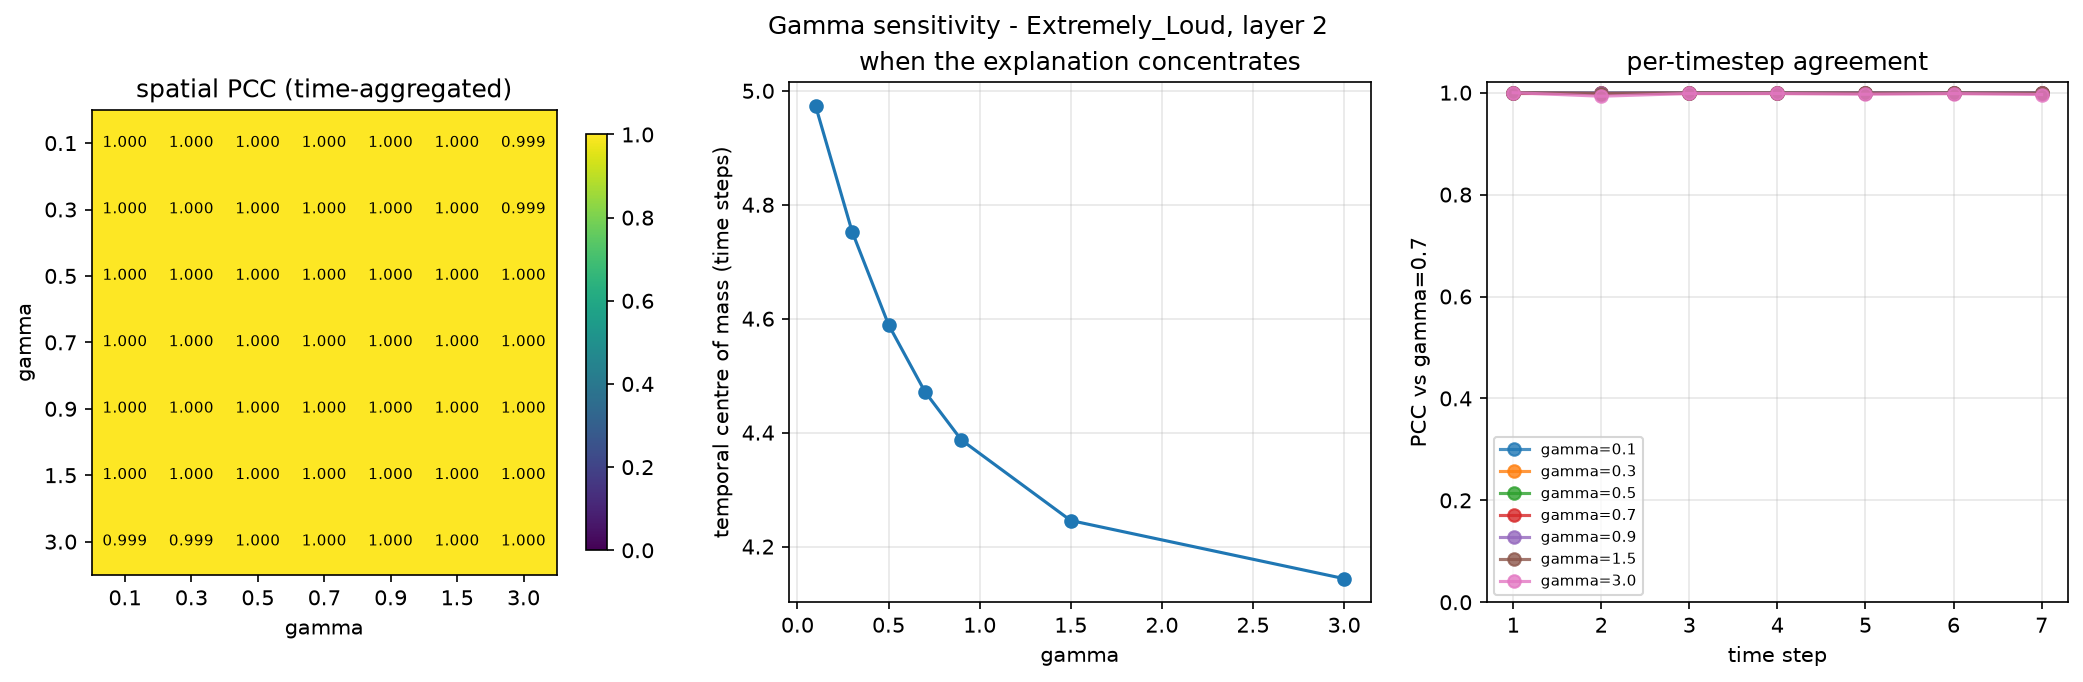
\includegraphics[width=\linewidth]{gamma_Extremely_Loud.png}\\[0.5em]
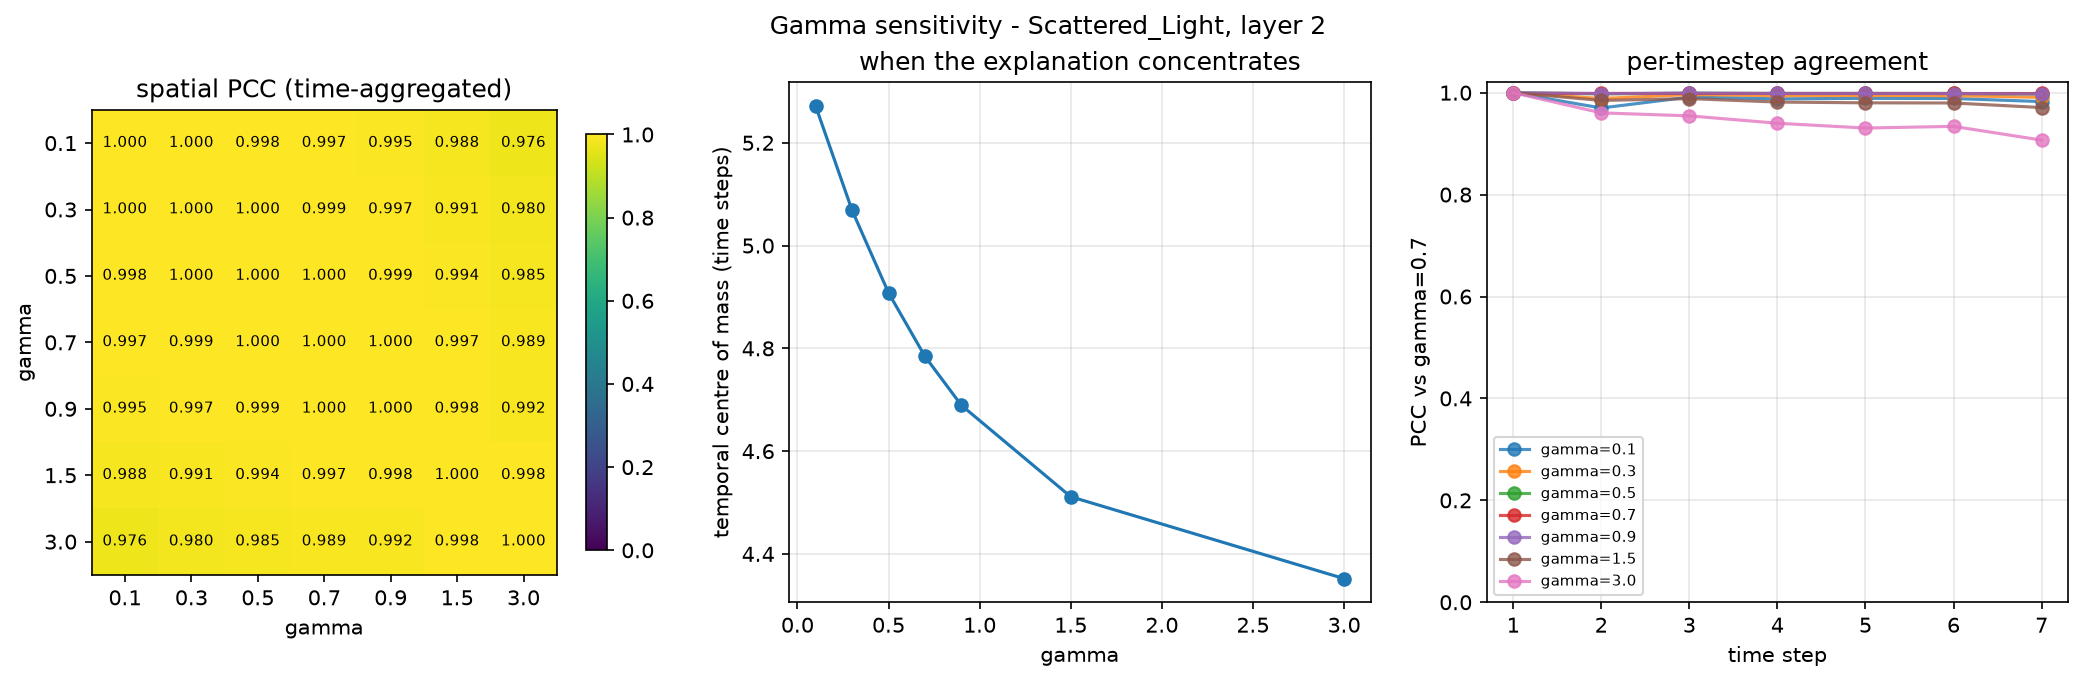
\includegraphics[width=\linewidth]{gamma_Scattered_Light.png}
\caption{$\gamma$ sensitivity at layer 2 for Blip, Extremely\_Loud and
Scattered\_Light (Violin\_Mode is in Figure~\ref{fig:gamma}).}
\label{fig:gamma-others}
\end{figure}

\begin{figure}[htbp]
\centering
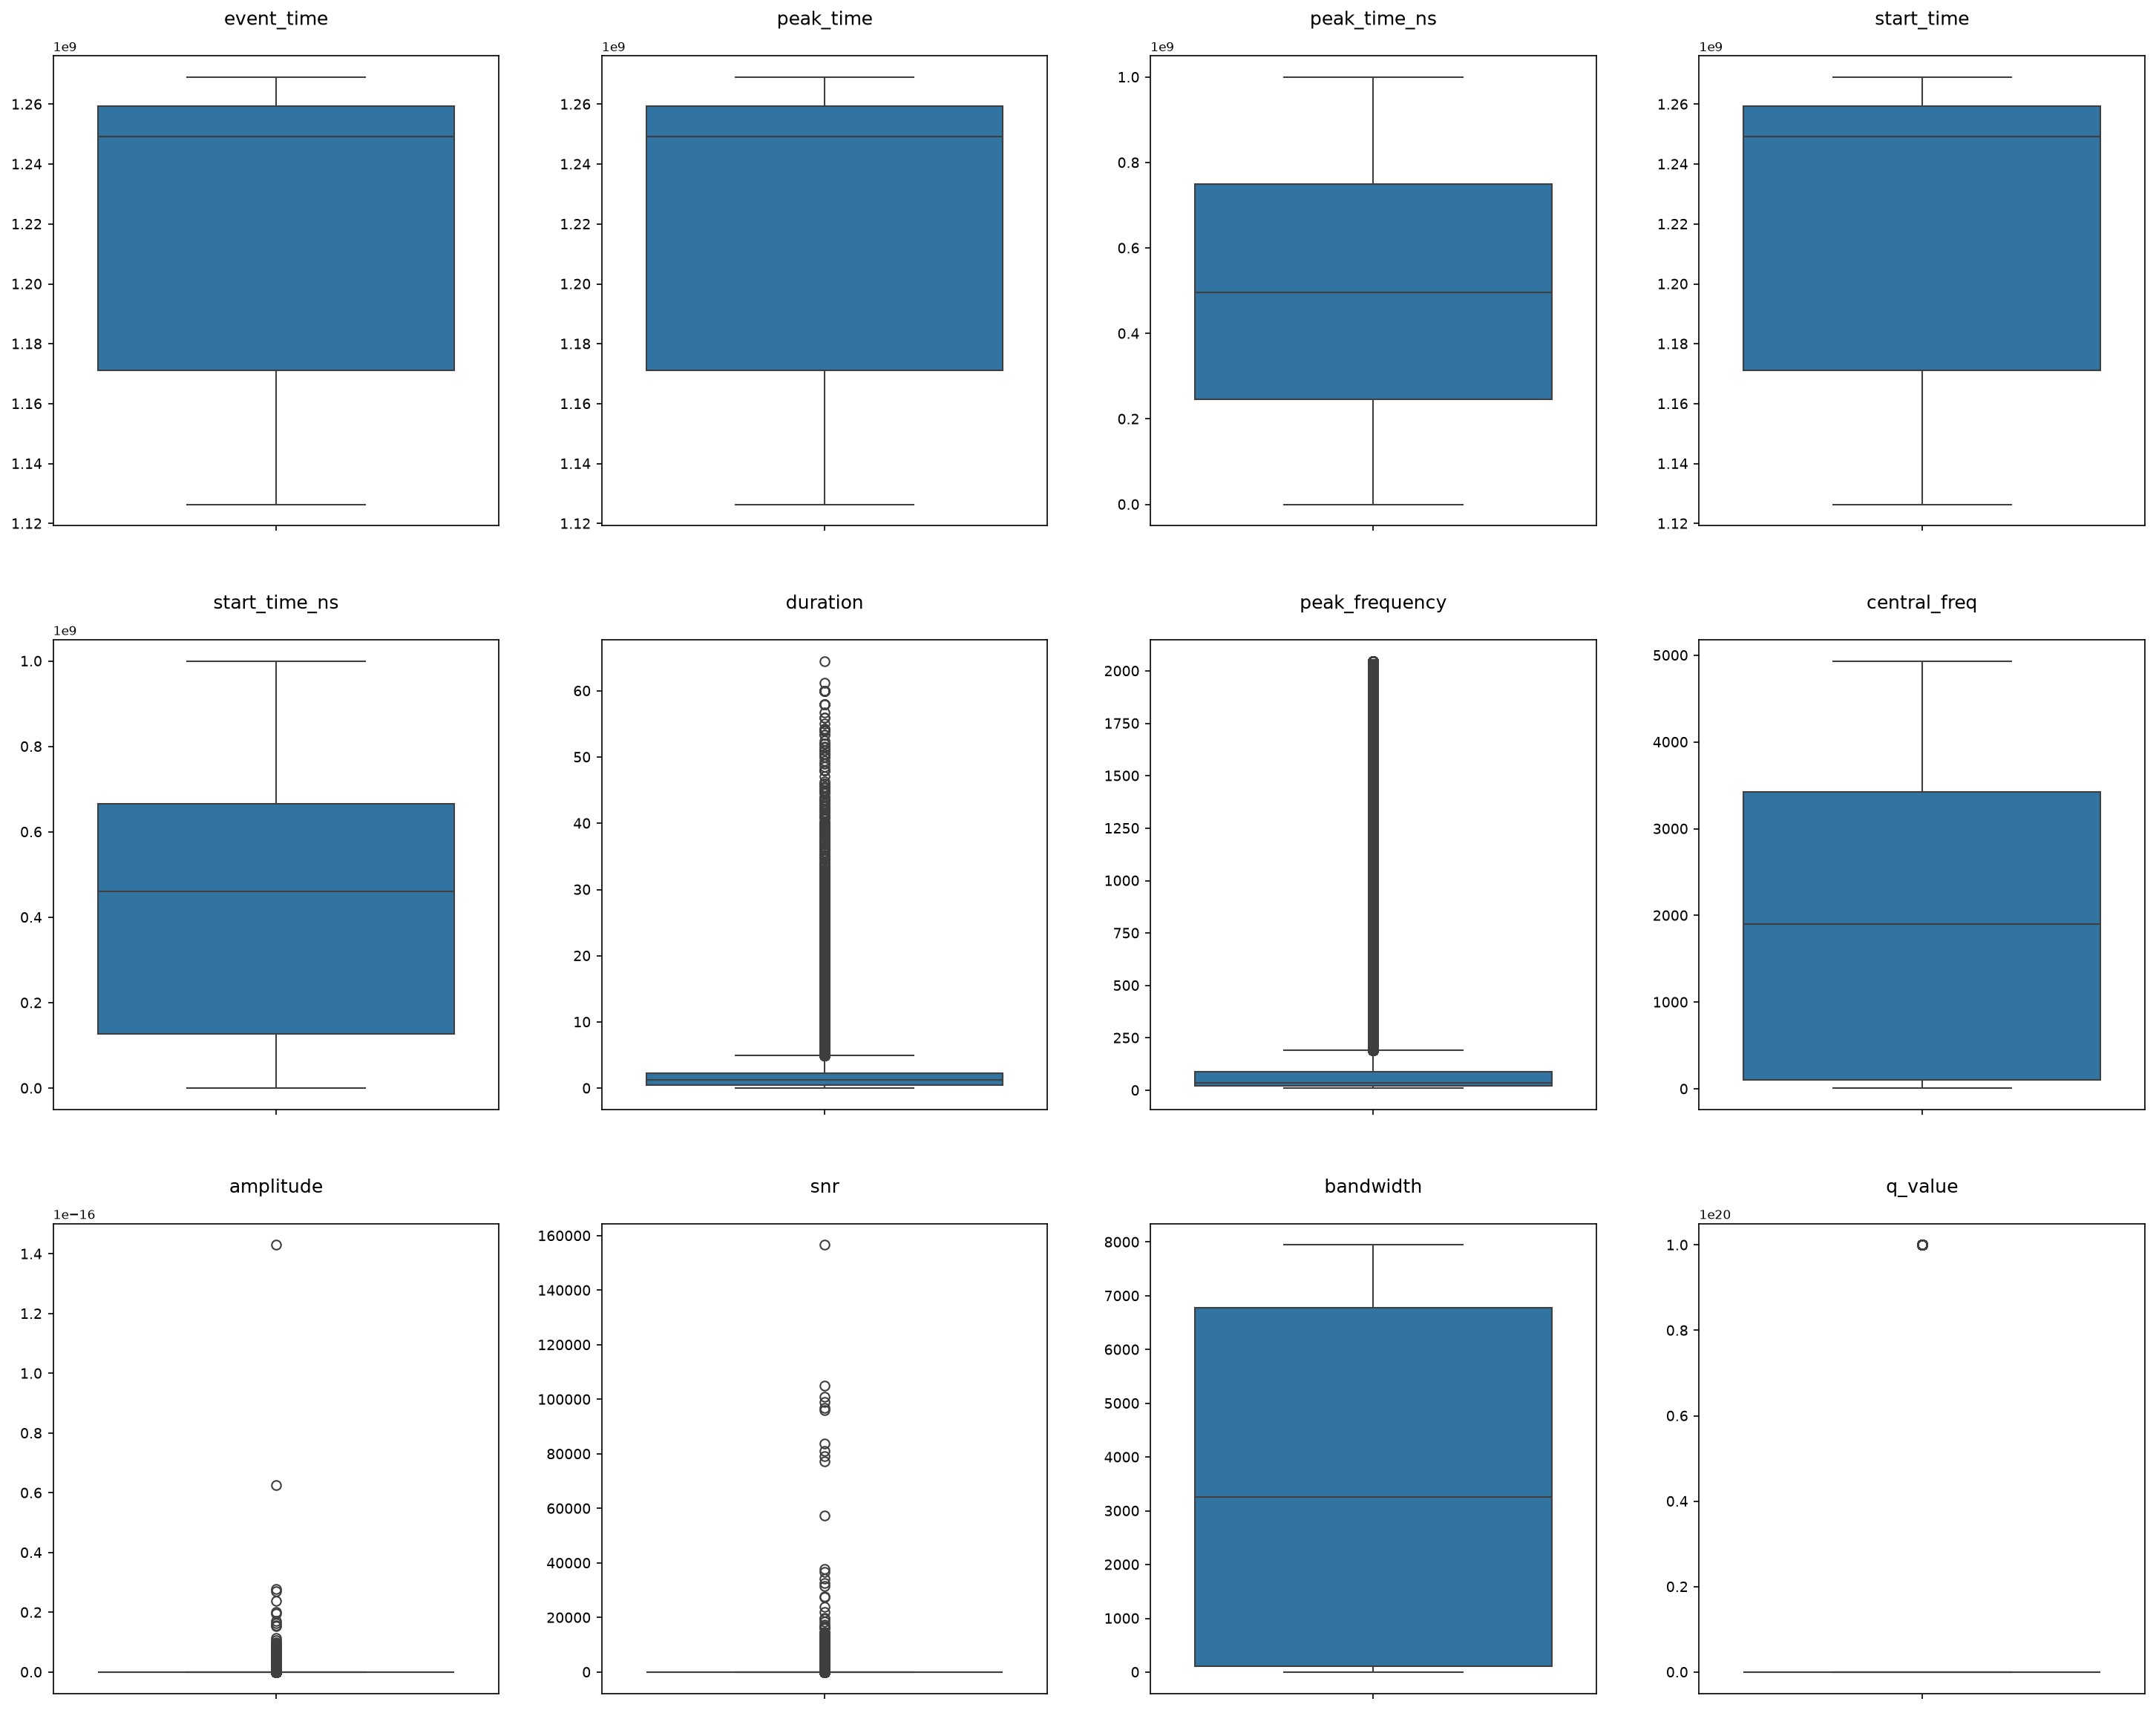
\includegraphics[width=\linewidth]{feature_boxplots.png}
\caption{Distributions of the twelve numerical Omicron descriptors over the full
release. The quality factor collapses to a sentinel value of order $10^{20}$;
amplitude and SNR are dominated by a long tail of outliers.}
\label{fig:boxplots}
\end{figure}

\chapter{Reproducibility}
\label{app:reproducibility}

All code, configuration and result files are in the public repository
\begin{center}\url{https://github.com/devs-glitch/Tesi}\end{center} Table~\ref{tab:repro} maps each
result of this thesis to the script that produces it and the file it writes.
Every script reads the model and the partition from
\texttt{config/baseline\_manifest.json}.

\begin{table}[htbp]
\centering
\small
\resizebox{\linewidth}{!}{%
\begin{tabular}{lll}
\toprule
Result & Script & Output \\
\midrule
Class selection, features & \texttt{scripts/data\_prep.py} & \texttt{selected\_dataset.csv} \\
Frozen partition & \texttt{scripts/freeze\_split.py} & \texttt{split\_assignment.csv} \\
Hyperparameter search & \texttt{scripts/tune.py} & \texttt{config/best\_hyperparams.json} \\
Resolution study & \texttt{scripts/resolution\_study.py} & \texttt{results/resolution\_study.csv} \\
FP32 reference & \texttt{scripts/fp32\_reference.py} & \texttt{config/baseline\_manifest.json} \\
Dead neurons & \texttt{scripts/dead\_neurons\_check.py} & \texttt{results/dead\_neurons.json} \\
Physical validation & \texttt{scripts/physical\_validation.py} & figures \\
$\gamma$ sensitivity & \texttt{xai/gamma\_sensitivity\_analysis.py} & \texttt{results/gamma\_sensitivity.json} \\
Deletion metric & \texttt{xai/deletion\_metric.py} & figure \\
Independent solutions & \texttt{xai/noise\_floor.py} & \texttt{results/noise\_floor.json} \\
Numerical floor & \texttt{xai/perturbation\_floor.py} & \texttt{results/perturbation\_floor.json} \\
Membrane range & \texttt{scripts/membrane\_range.py} & \texttt{config/membrane.json} \\
Clipping study & \texttt{scripts/test\_clipping.py} & \texttt{results/clipping\_test.json} \\
Quantizers & \texttt{model/quantization.py} & --- \\
\bottomrule
\end{tabular}}
\caption{From result to script.}
\label{tab:repro}
\end{table}

\todo{Add the rows for the grid (\texttt{grid\_runner.py},
\texttt{evaluate\_model.py}, \texttt{divergence\_metrics.py},
\texttt{cross\_faithfulness.py}, \texttt{stratify.py}, \texttt{energy.py},
\texttt{evaluate\_test.py}) once they exist, and check every path against the
final repository layout.}

%-------------------------------------------------------------------------------
\end{document}
%-------------------------------------------------------------------------------
